\begin{partbacktext}
\part{Многоагентные модели решателей задач интеллектуальных компьютерных систем нового поколения}

\vspace{-3\baselineskip}

\begin{SCn}
	\scnidtf{Часть 3. Многоагентные модели обработки различных видов знаний в интеллектуальных компьютерных системах нового поколения}
	\scnidtf{Часть 3. Принципы конвергенции и интеграции различных методов и моделей решения задач в многоагентных интеллектуальных компьютерных системах нового поколения}
	\scnidtf{Часть 3. Представление и обработка различных методов и моделей решения задач в многоагентных ostis-системах}
	
	\scntext{аннотация}{Уточнение понятий действия, задачи, метода, средства, навыка и технологии. Принципы программирования в ostis-системах. Принципы разработки различных видов решателей задач в многоагентных ostis-системах. Ситуационное управление в многоагентных ostis-системах. Базовый язык программирования для ostis-систем. Принципы конвергенции и интеграции различных моделей решения задач в ostis-системах.}
	
	\bigskip
	
	\begin{scnrelfromlist}{подраздел}
		\scnitem{Глава~\ref{chapter_actions}~\nameref{chapter_actions}}
		\scnitem{Глава~\ref{chapter_programs}~\nameref{chapter_programs}}
		\scnitem{Глава~\ref{chapter_situation_management}~\nameref{chapter_situation_management}}
		\scnitem{Глава~\ref{chapter_requests}~\nameref{chapter_requests}}
		\scnitem{Глава~\ref{chapter_logic_productions}~\nameref{chapter_logic_productions}}
		\scnitem{Глава~\ref{chapter_ann}~\nameref{chapter_ann}}
	\end{scnrelfromlist}
\end{SCn}

\end{partbacktext}

\chapter{Формализация понятий действия, задачи, метода, средства, навыка и технологии}
\chapauthortoc{Шункевич Д.В.\\Ковалёв М.В.}
\label{chapter_actions}

\vspace{-7\baselineskip}

\begin{SCn}
	\begin{scnrelfromlist}{автор}
		\scnitem{Шункевич Д.В.}
		\scnitem{Ковалёв М.В.}
	\end{scnrelfromlist}

	\bigskip

	\scntext{аннотация}{В главе уточнена формальная трактовка таких понятий, как \textit{действие}, \textit{задача}, \textit{класс действий}, \textit{класс задач}, \textit{метод}, \textit{навык}, что в совокупности позволило определить на их основе понятие \textit{модели решения задач}. Также уточнены понятия \textit{деятельности}, \textit{вида деятельности} и \textit{технологии}.}

	\bigskip

	\begin{scnrelfromlist}{подраздел}
		\scnitem{\ref{sec_action_concept}~\nameref{sec_action_concept}}
		\scnitem{\ref{sec_problem_concept}~\nameref{sec_problem_concept}}
		\scnitem{\ref{sec_action_and_problem_classes}~\nameref{sec_action_and_problem_classes}}
		\scnitem{\ref{sec_method_concept}~\nameref{sec_method_concept}}
		\scnitem{\ref{sec_skill_concept}~\nameref{sec_skill_concept}}
		\scnitem{\ref{sec_method_lang_concept}~\nameref{sec_method_lang_concept}}
		\scnitem{\ref{sec_problem_solving_model}~\nameref{sec_problem_solving_model}}
		\scnitem{\ref{sec_activity_and_technology}~\nameref{sec_activity_and_technology}}
	\end{scnrelfromlist}

	\bigskip

	\begin{scnrelfromlist}{ключевое понятие}
		\scnitem{воздействие}
		\scnitem{действие}
		\scnitem{задача}
		\scnitem{класс действий}
		\scnitem{класс задач}
		\scnitem{метод}
		\scnitem{язык представления методов}
		\scnitem{модель решения задач}
		\scnitem{навык}
		\scnitem{деятельность}
		\scnitem{вид деятельности}
		\scnitem{технология}
	\end{scnrelfromlist}

	\bigskip

	\begin{scnrelfromlist}{библиографическая ссылка}
		\scnitem{\scncite{Shunkevich2021}}
		\scnitem{\scncite{Standart2021}}
		\scnitem{\scncite{Fayans2020}}
		\scnitem{\scncite{Pospelov1986}}
		\scnitem{\scncite{Shunkevich2018}}
	\end{scnrelfromlist}

\end{SCn}

\section*{Введение в Главу \ref{chapter_actions}}
Возможности решателя задач интеллектуальной системы в значительной степени определяются качеством ее базы знаний. Другими словами, при разработке решателей задач необходимо описывать не только \textit{операционную семантику} решателя, то есть семейство интерпретаторов соответствующих моделей решения задач, но и \textit{декларативную семантику} модели решения задач, то есть собственно тексты программ (не программ низкоуровневых агентов, а программ более высокого уровня, интерпретируемых соответствующим набором агентов), логические утверждения, конкретные конфигурации искусственных нейронных сетей и так далее.

В рамках данной главы формально уточняются в рамках соответствующего набора онтологий такие понятия, как \textit{действие}, \textit{задача}, \textit{модель решения задач}, \textit{метод}, \textit{навык} и другие, на основе которых в \textit{Главе \ref{chapter_situation_management} \nameref{chapter_situation_management}} уточняется собственно модель гибридного \textit{решателя задач ostis-системы}.

%TODO Уточнить, будет ли где-то ранее говориться про sc-агенты и многоагентный подход
Разработка указанного семейства онтологий позволяет:
\begin{textitemize}
	\item явно связать \textit{класс задач} и способ (метод) решения задач данного класса;
	\item это, в свою очередь, позволит накапливать более сложные компоненты решателей задач и еще больше упростить их интеграцию, поскольку вместе с коллективом sc-агентов в соответствующий компонент также будут входить необходимые фрагменты базы знаний, априори согласованные с указанным коллективом sc-агентов;
	\item это, в свою очередь, позволит сделать средства автоматизации разработки решателей задач более интеллектуальными, в частности, позволит автоматизировать процесс подбора компонентов решателя на основе спецификации классов задач, которые должна уметь решать проектируемая интеллектуальная система;
	\item в дальнейшем это позволит интеллектуальной системе самостоятельно обращаться в библиотеку компонентов решателей задач (см. \ref{sec_ps_components}~\nameref{sec_ps_components}) и подбирать компоненты, исходя из новых классов задач, с которыми столкнулась система, то есть позволит интеллектуальной системе самостоятельно изучать новые \textit{навыки};
	\item с другой стороны, такой подход позволит интеллектуальной системе самостоятельно подобрать комбинацию моделей решения задач для решения задач определенного класса (точнее говоря, поскольку в основу решателя положен многоагентный подход, то коллектив sc-агентов, интерпретирующих различные модели решения задач, сможет лучше определить, какие именно из sc-агентов и в каком порядке должны работать при решении конкретной комплексной задачи).
\end{textitemize}

Результаты, ранее полученные авторами в данной области исследований опубликованы в таких работах, как \scncite{Shunkevich2021}, \scncite{Standart2021}.

\section{Понятие действия}
\label{sec_action_concept}

\begin{SCn}
	\begin{scnrelfromlist}{ключевое понятие}
		\scnitem{воздействие}
		\scnitem{действие}
		\scnitem{субъект}
		\scnitem{информационное действие}
		\scnitem{поведенческое действие}
		\scnitem{эффекторное действие}
		\scnitem{рецепторное действие}
		\scnitem{атомарное действие}
		\scnitem{неатомарное действие}
	\end{scnrelfromlist}

	\begin{scnrelfromlist}{ключевое отношение}
		\scnitem{субъект\scnrolesign}
		\scnitem{объект\scnrolesign}
		\scnitem{цель*}
	\end{scnrelfromlist}
\end{SCn}

Прежде чем говорить о моделях решения задач и решателя задач, необходимо формально уточнить понятие задачи и понятие действия, направленного на решение той или иной задачи или ее подзадач.

В рамках \textit{Технологии OSTIS} задачу будем трактовать как формальную спецификацию некоторого действия, поэтому целесообразно вначале уточнить понятие \textbf{\textit{действия}}, которое определяется через понятие \textbf{\textit{воздействия}}. Рассмотрим спецификацию понятия \textit{воздействие} в SCn-коде.

\begin{SCn}
	\scnheader{воздействие}
	\scnidtf{\textit{процесс} воздействия одной сущности (или некоторого множества \textit{сущностей}) на другую \textit{сущность} (или на некоторое множество других \textit{сущностей})}
	\scnidtf{\textit{процесс}, в котором могут быть явно выделены хотя бы одна воздействующая сущность (\textit{субъект\scnrolesign}) и хотя бы одна \textit{сущность}, на которую осуществляется воздействие (\textit{объект\scnrolesign})}
	\scnidtf{акция}
	\scnsubset{процесс}
	\begin{scnindent}
		\scnidtf{динамическая структура}
	\end{scnindent}

	\scnheader{субъект}
	\scnidtf{активная сущность}
	\scnsubset{сущность}
	\scnidtftext{часто используемый sc-идентификатор}{индивид}

	\scnheader{субъект\scnrolesign}
	\scnidtf{воздействующая сущность\scnrolesign}
	\scnidtf{сущность, создающая \textit{причину} изменений другой сущности (объекта)\scnrolesign}

	\scnheader{объект\scnrolesign}
	\scnidtf{воздействуемая сущность\scnrolesign}
	\scnidtf{сущность, являющаяся в рамках заданного воздействия исходным условием (аргументом), необходимым для выполнения этого воздействия\scnrolesign}
\end{SCn}

Каждому \textit{воздействию} может быть поставлен в соответствие (1) некоторый \textit{субъект\scnrolesign}, то есть сущность, осуществляющая \textit{воздействие} (в частности, это может быть некоторое физическое поле), и (2) некоторый \textit{объект\scnrolesign}, то есть сущность, на которую воздействие направлено. Если \textit{воздействие} связано с \textit{материальной сущностью}, то его объектом является либо сама эта \textit{материальная сущность}, либо некоторая ее пространственная часть.

Поскольку \textit{воздействия} являются частным видом \textit{процессов}, воздействиями наследуются все свойства \textit{процессов}. В частности, используются все \textit{параметры}, заданные на множестве \textit{процессов}, например, \textit{длительность*}, \textit{момент начала процесса*}, \textit{момент завершения процесса\scnsupergroupsign}. Подробнее эти отношения описываются в \textit{Главе \ref{chapter_top_ontologies} \nameref{chapter_top_ontologies}}.

Также, так как воздействие является процессом и, соответственно, представляет собой \textit{динамическую структуру}, то и знак \textit{субъекта воздействия\scnrolesign}, и знак \textit{объекта воздействия\scnrolesign} являются элементами данной структуры. В связи с этим можно рассматривать отношения \textit{субъект воздействия\scnrolesign} и \textit{объект воздействия\scnrolesign} как \textit{ролевые отношения}. Данный факт не запрещает вводить аналогичные \textit{неролевые отношения}, однако это нецелесообразно.

Рассмотрим спецификацию понятия \textit{действие} в SCn-коде.
\begin{SCn}
	\scnheader{действие}
	\scnidtf{\textit{воздействие}, в котором \textit{субъект\scnrolesign} осуществляет \textit{воздействие} целенаправленно, то есть в соответствии с некоторой \textit{целью*}}
	\scnidtf{целенаправленное воздействие, выполняемое одним или несколькими субъектами (кибернетическими системами) с возможным применением некоторых инструментов}
	\scnidtf{акт}
	\scnidtf{операция}
	\scnidtf{осознанное воздействие}
	\scnidtf{активное воздействие}
	\scnsubset{воздействие}
	\begin{scnindent}
		\scnidtf{процесс, в котором могут быть явно выделены хотя бы одна воздействующая сущность (субъект воздействия\scnrolesign) и хотя бы одна сущность, на которую осуществляется воздействие (объект воздействия\scnrolesign)}
		\scnsubset{процесс}
	\end{scnindent}

	\scnidtf{целенаправленный (\scnqq{осознанный}) процесс, выполняемый (управляемый, реализуемый) неким субъектом}
	\scnidtf{работа}
	\scnidtf{процесс решения некоторой задачи}
	\scnidtf{процесс достижения некоторой цели}
	\scnidtf{целостный фрагмент некоторой деятельности}
	\scnidtf{целенаправленный процесс, управляемый некоторым субъектом}
	\scnidtf{процесс выполнения некоторого действия некоторым субъектом (исполнителем) над некоторыми объектами}

	\scnheader{цель*}
	\scnidtf{целевая ситуация*}
	\scnsubset{спецификация*}
	\scnidtf{описание того, что требуется получить (какая ситуация должна быть достигнута) в результате выполнения заданного (специфицируемого) действия*}
\end{SCn}

Каждое \textit{действие}, выполняемое тем или иным \textit{субъектом}, трактуется как процесс решения некоторой задачи, то есть процесс достижения заданной \textit{цели*} в заданных условиях, и, следовательно, выполняется целеноправленно. При этом явное указание \textit{действия} и его связи с конкретной задачей может не всегда присутствовать в памяти. Некоторые \textit{задачи} могут решаться определенными субъектами перманентно, например, оптимизация \textit{базы знаний}, поиск некорректностей и так далее и для подобных задач не всегда есть необходимость явно вводить \textit{структуру}, являющуюся формулировкой \textit{задачи}.

Каждое \textit{действие} может обозначать сколь угодно малое преобразование, осуществляемое во внешней среде либо в памяти некоторой \textit{кибернетической системы}, однако в памяти явно вводятся знаки только тех \textit{действий}, для которых есть небходимость явно хранить в памяти их спецификацию в течение некоторого времени.

При выполнении \textit{действия} можно выделить этапы:
\begin{scnitemize}
	\item построение \textit{плана действия}, декомпозиция (детализация) действия в виде системы его \textit{поддействий};
	\item выполнение построенного плана \textit{действия}.
\end{scnitemize}

Класс действий имеет разбиение по следующим признакам:
\begin{scnitemize}
	\item место выполнения действия;
	\item функциональная сложность действия;
	\item многоагентность выполнения действия;
	\item текущее состояние действия.
\end{scnitemize}

Далее рассмотрим разбиение по каждому признаку.

\begin{SCn}
	\scnheader{действие}
	\scnrelfrom{разбиение}{Типология классов действий по признаку места выполнения действия}
	\begin{scnindent}
		\begin{scneqtoset}
			\scnitem{информационное действие}
			\begin{scnindent}
				\scnidtf{действие, выполняемое в памяти субъекта действия}
				\scnidtf{действие, выполняемое в памяти}
				\scnidtf{действие кибернетической системы, направленное на обработку информации, хранимой в её памяти}
			\end{scnindent}
			\scnitem{поведенческое действие}
			\begin{scnindent}
				\scnidtf{действие, выполняемое во внешней среде субъекта действия}
			\end{scnindent}
			\scnitem{рецепторное действие}
			\begin{scnindent}
				\scnidtf{сенсорное действие}
			\end{scnindent}
			\scnitem{эффекторное действие}
		\end{scneqtoset}
	\end{scnindent}
\end{SCn}

Результатом выполнения \textbf{\textit{информационного действия}} в общем случае является некоторое новое состояние памяти информационной системы (не обязательно \textit{sc-памяти}), достигнутое исключительно путем преобразования информации, хранящейся в памяти системы, то есть либо посредством генерации новых знаний на основе уже имеющихся, либо посредством удаления знаний, по каким-либо причинам ставших ненужными. Следует отметить, что если речь идет об изменении состояния \textit{sc-памяти}, то любое преобразование информации можно свести к ряду атомарных действий по генерации, удалению или изменению инцидентности \textit{sc-элементов} относительно друг друга.

В случае \textbf{\textit{поведенческого действия}} результатом его выполнения будет новое состояние внешней среды. Очень важно отметить, что под внешней средой в данном случае понимаются также и компоненты системы, внешние с точки зрения памяти, то есть не являющиеся хранимыми в ней информационными конструкциями. К таким компонентам можно отнести, например, различные манипуляторы и прочие средства воздействия системы на внешний мир, то есть к поведенческим задачам можно отнести изменение состояния механической конечности робота или непосредственно вывод некоторой информации на экран для восприятия пользователем.

Каждое \textbf{\textit{рецепторное действие}} обозначает класс \textit{действий}, которые осуществляют преобразования в памяти субъекта действия под воздействием внешней среды.

Соответственно, каждое \textbf{\textit{эффекторное действие}} обозначает класс \textit{действий}, которые осуществляют преобразования внешней среды под воздействием памяти субъекта воздействия.

Также действия могут разбиваться по признаку их функциональной сложности.
\begin{SCn}
	\scnheader{действие}
	\scnrelfrom{разбиение}{Типология классов действий по признаку функциональной сложности действия}
	\begin{scnindent}
		\begin{scneqtoset}
			\scnitem{атомарное действие}
			\begin{scnindent}
				\scnidtf{элементарное действие}
			\end{scnindent}
			\scnitem{неатомарное действие}
			\begin{scnindent}
				\scnidtf{неэлементарное действие}
				\scnidtf{неатомарное действие}
				\begin{scnrelfromset}{покрытие}
					\scnitem{легко выполнимое неатомарное действие}
					\scnitem{трудно выполнимое неатомарное действие}
					\begin{scnindent}
						\scnidtf{интеллектуальное действие}
					\end{scnindent}
				\end{scnrelfromset}
			\end{scnindent}
		\end{scneqtoset}
	\end{scnindent}
\end{SCn}

Разберем подробнее каждый элемент приведенной иерархии.
\textbf{\textit{атомарное действие}}  выполняется одним индивидуальным субъектом и не включает в себя выполнение каких-либо дочерних действий.

Соответственно, \textbf{\textit{неатомарное действие}} является действием, выполнение которого требует декомпозиции этого действия на множество его \uline{поддействий}, то есть частных действий более низкого уровня. Более частные действия могут выполняться как последовательно, так и параллельно.

Декомпозиция неатомарного действия на поддействия может иметь весьма сложный иерархический вид с большим числом уровней иерархии, то есть поддействиями \textit{неатомарного действия} могут быть также \textit{неатомарные действия}. Уровень сложности действия можно определять (1) общим числом его поддействий и (2) числом уровней иерархии этих поддействий. Примером может служить запись одной и той же процедурной программы на языке программирования более высокого уровня и на языке программирования более низкого уровня. В данном случае атомарность действий строго определяется на уровне языка.

Темпоральные соотношения между \textit{поддействиями} неатомарного \textit{действия} могут быть самые различные, но в пройстейшем случае \textit{неатомарное действие} представляет собой строгую последовательность \textit{действий} более низкого уровня иерархии.

В состав \textit{неатомарного действия} могут входить не только \textit{собственно поддействия} этого \textit{неатомарного действия}, но также и специальные \textit{поддействия}, осуществляющие \uline{управление} процессом выполнения \textit{неатомарного действия}, и, в частности, \textit{поддействия}, осуществляющие инициирование поддействий, передачу управления \textit{поддействиям}.

Действие можно назвать \textbf{\textit{легко выполнимым неатомарным действием}} в случае, когда для выполнения этого действия известен соответствующий \textit{метод} и соответствующие этому методу исходные данные, а также (для действий, выполняемых во внешней среде) имеются в наличии все необходимые исходные объекты (расходные материалы и комплектация), а также средства (инструменты).

В свою очередь, \textbf{\textit{трудно выполнимым неатомарным действием}} действие является тогда, когда для его выполнения в текущий момент либо неизвестен соответствующий \textit{метод}, либо возможные \textit{методы} известны, но отсутствуют условия их применения. Это действие декомпозируется на несколько самостоятельных поддействий, каждое из которых выявляет (локализует) противоречия (ошибки) конкретного формализуемого вида, для которого в базе знаний существует точное определение.

Признак многоагентности выполнения действия характеризует количество субъектов, выполнеяющих действие.
\begin{SCn}
	\scnheader{действие}
	\scnrelfrom{разбиение}{Типология классов действий по признаку многоагентности выполнения действия}
	\begin{scnindent}
		\begin{scneqtoset}
			\scnitem{индивидуальное действие}
			\begin{scnindent}
				\scnidtf{действие, выполняемое одним субъектом (агентом)}
				\scnidtf{действие, выполняемое индивидуальной кибернетической системой}
			\end{scnindent}
			\scnitem{коллективное действие}
			\begin{scnindent}
				\scnidtf{действие, выполняемое коллективом субъектов (многоагентной системой)}
				\scnidtf{действие, выполняемое коллективом кибернетических систем (коллективом субъектов)}
				\scnsuperset{действие, выполняемое коллективом людей}
				\scnsuperset{действие, выполняемое коллективом индивидуальных компьютерных систем}
				\scnsuperset{действие, выполняемое коллективом людей и индивидуальных компьютерных систем}
				\begin{scnindent}
					\scnsuperset{действие, выполняемое Экосистемой OSTIS}
					\scnsuperset{действие, выполняемое одним человеком во взаимодействии с одной индивидуальной компьютерной системой}
				\end{scnindent}
			\end{scnindent}
		\end{scneqtoset}
	\end{scnindent}
\end{SCn}

Последним признаком разбиения классов действия является признак текущего состояния действия.
\begin{SCn}
	\scnheader{действие}
	\scnrelfrom{разбиение}{Типология классов действий по признаку текущего состояния действия}
	\begin{scnindent}
		\begin{scneqtoset}
			\scnitem{планируемое действие}
			\begin{scnindent}
				\scnidtf{запланированное, но не инициированное действие}
				\scnidtf{будущее действие}
			\end{scnindent}
			\scnitem{инициированное действие}
			\begin{scnindent}
				\scnidtf{действие, ожидающее начала своего выполнения}
				\scnidtf{действие, подлежащее выполнению}
			\end{scnindent}
			\scnitem{выполняемое действие}
			\begin{scnindent}
				\scnidtf{активное действие}
				\scnidtf{действие, выполняемое в текущий момент}
				\scnidtf{настоящее действие}
			\end{scnindent}
			\scnitem{прерванное действие}
			\begin{scnindent}
				\scnidtf{действие, ожидающее продолжения своего выполнения}
				\scnidtf{отложенное действие}
			\end{scnindent}
			\scnitem{выполненное действие}
			\begin{scnindent}
				\scnidtf{завершенное действие}
				\scnidtf{прошлое действие}
				\begin{scnsubdividing}
					\scnitem{успешно выполненное действие}
					\scnitem{безуспешно выполненное действие}
					\begin{scnindent}
						\scnsuperset{действие, выполненное с ошибкой}
					\end{scnindent}
				\end{scnsubdividing}
			\end{scnindent}
			\scnitem{отмененное действие}
		\end{scneqtoset}
	\end{scnindent}
\end{SCn}

Во множество \textbf{\textit{планируемых действий}} входят \textit{действия}, начало выполнение которых запланировано на какой-либо момент в будущем(\textit{начало*}).

Во множество \textbf{\textit{инициированных действий}} входят \textit{действия}, выполнение которых инициировано в результате какого-либо события.
В общем случае, \textit{действия} могут быть инициированы по следующим причинам:
\begin{scnitemize}
	\item явно путем проведения соответствующей \textit{sc-дуги принадлежности} каким-либо \textit{субъектом (заказчиком*)}. В случае действия в \textit{sc-памяти}, оно может быть инициировано как внутренним \textit{sc-агентом} системы, так и пользователем при помощи соответствующего пользовательского интерфейса. При этом, спецификация действия может быть сформирована одним \textit{sc-агентом}, а собственно добавление во множество \textit{инициированных действий} может быть осуществлено позже другим \textit{sc-агентом};
	\item в результате того, что одно или несколько \textit{действий}, предшествовавших данному в рамках некоторой декомпозиции, стали \textit{прошлыми сущностями} (процедурный подход);
	\item в результате того, что в \textit{памяти} системы появилась конструкция, соответствующая некоторому условию инициирования \textit{sc-агента}, который должен выполнить данное \textit{действие} (декларативный подход).
\end{scnitemize}

Следует отметить, что декларативный и процедурный подходы можно рассматривать как две крайности, использование только одной из которых не является удобным и целесообразным. При этом, например, принципы инициирования по процедурному подходу могут быть полностью сведены к набору декларативных условий инициирования, но как было сказано, это не всегда удобно и наиболее рациональным будет комбинировать оба подхода в зависимости от ситуации.

Принадлежность некоторого \textit{действия} множеству \textit{инициированных действий} говорит о том, что, по мнению некоторого \textit{субъекта} (заказчика, инициатора), оно готово к выполнению и должно быть выполнено, то есть спецификация данного \textit{действия} по мнению данного \textit{субъекта} сформирована в степени, достаточной для решения поставленной \textit{задачи} и существует некоторый другой \textit{субъект} (исполнитель), который может приступать к выполнению \textit{действия}. Однако стоит отметить, что с точки зрения \textit{исполнителя} такая спецификация \textit{действия} в общем случае может оказаться недостаточной или некорректной.

Во множество \textbf{\textit{выполняемых действий}} входят \textit{действия}, к выполнению которых приступил какой-либо из соответствующих \textit{субъектов}.
Попадание \textit{действия} в данное множество говорит о следующем:
\begin{scnitemize}
	\item рассматриваемое \textit{действие} уже попало во множество \textit{инициированных действий};
	\item существует как минимум один \textit{субъект}, условие инициирования которого соответствует спецификации данного \textit{действия}.
\end{scnitemize}

После того, как собственно процесс выполнения завершился, \textit{действие} должно быть удалено из множества \textit{выполняемых действий} и добавлено во множество \textit{выполненных действий} или какое-либо из его подмножеств.

Понятие \textit{выполняемое действие} является неосновным, и вместо того, чтобы относить конкретные действия к данному классу, их относят к классу \textit{настоящих сущностей}.

Во множество \textbf{\textit{прерванных действий}} входят \textit{действия}, которые уже были инициированы, однако их выполнение невозможно по каким-либо причинам, например в случае, когда у исполнителя в данный момент есть более приоритетные задачи.

Во множество \textbf{\textit{выполненных действий}} попадают \textit{действия}, выполнение которых завершено с \uline{точки зрения \textit{субъекта}}, осуществлявшего их выполнение. Таким образом, понятие \textit{выполненного действия} является относительным, поскольку с точки зрения разных субъектов одно и то же действие может считаться выполненным или все еще выполняющимся.

В зависимости от результатов конкретного процесса выполнения, рассматриваемое \textit{действие} может стать элементом одного из подмножеств множества \textit{выполненных действий}.

Понятие \textit{выполненное действие} является неосновным, и вместо того, чтобы относить конкретные \textit{действия} к данному классу, их относят к классу \textit{прошлых сущностей}.

Во множество \textbf{\textit{успешно выполненных действий}} попадают \textit{действия}, выполнение которых успешно завершено с точки зрения \textit{субъекта}, осуществлявшего их выполнение, то есть достигнута поставленная цель, например, получены решение и ответ какой-либо задачи, успешно преобразована какая-либо конструкция и так далее. Очень важно отметить, что в общем случае выделить критерии успешности или безуспешности выполнения действий того или иного класса \uline{невозможно}, поскольку эти критерии, во-первых, зависят от контекста, во-вторых, могут быть разными с точки зрения разных субъектов. Однозначно критерии успешности выполнения действий могут быть сформулированы для некоторых частных классов действий, например, классов операторов некоторого процедурного языка программирования (например, \textit{scp-операторов}). Таким образом, понятие \textit{успешно выполненное действие} является относительным.

Если действие было выполнено успешно, то, в случае действия по генерации каких-либо знаний, к \textit{действию} при помощи связки отношения \textit{результат*} приписывается \textit{sc-конструкция}, описывающая результат выполнения указанного действия. В случае, когда действие направлено на какие-либо изменения базы знаний, \textit{sc-конструкция}, описывающая результат действия, формируется в соответствии с правилами описания истории изменений базы знаний.

В случае, когда успешное выполнение \textit{действия} приводит к изменению какой-либо конструкции в \textit{sc-памяти}, которое необходимо занести в историю изменений базы знаний или использовать для демонстрации протокола решения задачи, то генерируется соответствующая связка отношения \textit{результат*}, связывающая задачу и \textit{sc-конструкцию}, описывающую данное изменение.

Во множество \textbf{\textit{безуспешно выполненных действий}} попадают \textit{действия}, выполнение которых не было успешно завершено с точки зрения \textit{субъекта}, осуществлявшего их выполнение, по каким-либо причинам.

Можно выделить две основные причины, по которым может сложиться указанная ситуация:
\begin{scnitemize}
	\item соответствующая \textit{задача} сформулирована некорректно;
	\item формулировка соответствующей \textit{задачи} корректна и понятна системе, однако решение данной задачи в текущий момент не может быть получено за удовлетворительные с точки зрения заказчика или исполнителя сроки.
\end{scnitemize}

Для конкретизации факта некорректности формулировки задачи можно выделить ряд более частных классов \textit{безуспешно выполненных действий}, например:
\begin{scnitemize}
	\item \textit{действие, спецификация которого противоречит другим знаниям системы} (например, не выполняется неравенство треугольника);
	\item \textit{действие, при спецификации которого использованы понятия, неизвестные системе};
	\item \textit{действие, выполнение которого невозможно из-за недостаточности данных} (например, найти площадь треугольника по двум сторонам);
	\item и другие.
\end{scnitemize}

Для конкретизации факта безуспешности выполнения некоторого действия в системе могут также использоваться дополнительные подмножества данного множества, при необходимости снабженные естественно-языковыми или формальными комментариями.

Во множество \textbf{\textit{действий, выполненных с ошибкой}}, попадают \textit{действия}, выполнение которых не было успешно завершено с точки зрения \textit{субъекта}, осуществлявшего их выполнение, по причине возникновения какой-либо ошибки, например, некорректности спецификации данного \textit{действия} или нарушения её целостности каким-либо \textit{субъектом} (в случае \textit{действия в sc-памяти}).


\section{Понятие задачи}
\label{sec_problem_concept}

\begin{SCn}
	\begin{scnrelfromlist}{ключевое понятие}
		\scnitem{задача}
		\scnitem{информационная задача}
		\scnitem{поведенческая задача}
		\scnitem{декларативная формулировка задачи}
		\scnitem{процедурная формулировка задачи}
		\scnitem{декларативно-процедурная формулировка задачи}
		\scnitem{вопрос}
		\scnitem{команда}
	\end{scnrelfromlist}

	\begin{scnrelfromlist}{ключевое отношение}
		\scnitem{спецификация*}
		\scnitem{декларативная формулировка задачи*}
		\scnitem{процедурная формулировка задачи*}
	\end{scnrelfromlist}
\end{SCn}

Понятие \textbf{\textit{задача}} будем трактовать как спецификацию некоторого действия, в рамках которой, в зависимости от ситуации, при помощи перечисленных выше отношений может быть заранее указан контекст выполнения действия, способ его выполнения, исполнитель, заказчик, планируемый результат и так далее

Рассмотрим спецификацию понятия \textit{задача} в SCn-коде.

\begin{SCn}
	\scnheader{задача}
	\scnidtf{описание некоторого желаемого состояния или события либо в базе знаний, либо во внешней среде}
	\scnidtf{формулировка задачи}
	\scnidtf{задание на выполнение некоторого действия}
	\scnidtf{постановка задачи}
	\scnidtf{задачная ситуация}
	\scnidtf{спецификация некоторого действия, обладающая достаточной полнотой для выполнения этого действия}
\end{SCn}

Формальное описание условия некоторой \textit{задачи есть}, по сути, формальная \textit{спецификация} некоторого \textit{действия}, направленного на решение данной \textit{задачи}, достаточная для выполнения данного \textit{действия} каким-либо \textit{субъектом}.

Каждая \textbf{\textit{задача}} представляет собой спецификацию действия, которое либо уже выполнено, либо выполняется в текущий момент (в настоящее время), либо планируется (должно) быть выполненным, либо может быть выполнено (но не обязательно). В зависимости от конкретного класса задач, описываться может как внутреннее состояние самой интеллектуальной системы, так и требуемое состояние внешней среды.

Классификация задач может осуществляться по дидактическому признаку в рамках каждой предметной области, например, задачи на треугольники, задачи на системы уравнений и тому подобное.

Каждая \textit{задача} может включать:
\begin{textitemize}
	\item факт принадлежности \textit{действия} какому-либо частному классу \textit{действий} (например,\textit{ действие. сформировать полную семантическую окрестность указываемой сущности}), в том числе состояние \textit{действия} с точки зрения жизненного цикла (инициированное, выполняемое и так далее);
	\item описание \textit{цели*} (\textit{результата*}) \textit{действия}, если она точно известна;
	\item указание \textit{заказчика*} действия;
	\item указание \textit{исполнителя* действия} (в том числе коллективного);
	\item указание \textit{аргумента(-ов) действия\scnrolesign};
	\item указание инструмента или посредника \textit{действия};
	\item описание \textit{декомпозиции действия*};
	\item указание \textit{последовательности действий*} в рамках \textit{декомпозиции действия*}, то есть построение процедурного плана решения задачи. Другими словами, построение плана решения представляет собой декомпозицию соответствующего \textit{действия} на систему взаимосвязанных между собой поддействий;
	\item указание области \textit{действия};
	\item указание условия инициирования \textit{действия};
	\item момент начала и завершения \textit{действия}, в том числе планируемый и фактический, предполагаемая и/или фактическая длительность выполнения.
\end{textitemize}
Некоторые задачи могут быть дополнительно уточнены контекстом --- дополнительной информацией о сущностях, рассматриваемых в формулировке \textit{задачи}, то есть описанием того, что дано, что известно об указанных сущностях.

Кроме этого, \textit{задача} может включать любую дополнительную информацию о действии, например:
\begin{textitemize}
	\item перечень ресурсов и средств, которые предполагается использовать при решении задачи, например, список доступных исполнителей, временные сроки, объем имеющихся финансов и так далее;
	\item ограничение области, в которой выполняется \textit{действие}, например, необходимо заменить одну \textit{sc-конструкцию} на другую по некоторому правилу, но только в пределах некоторого \textit{раздела базы знаний};
	\item ограничение знаний, которые можно использовать для решения той или иной задачи, например, необходимо решить задачу по алгебре, используя только те утверждения, которые входят в курс школьной программы до седьмого класса включительно, и не используя утверждения, изучаемые в старших классах;
	\item и прочее.
\end{textitemize}

Как и в случае с действиями, решаемыми системой, можно классифицировать \textit{информационные задачи} и \textit{поведенческие задачи}.

С другой стороны, с точки зрения формулировки поставленной задачи, можно выделить \textit{декларативные формулировки задачи} и \textit{процедурные формулировки задачи}. Следует отметить, что данные классы задач не противопоставляются друг другу, и могут существовать формулировки задач, использующие оба подхода.

\begin{SCn}
	\scnheader{задача}
		\scnsuperset{вопрос}
		\scnsuperset{команда}
		\scnsubset{знание}
		\scnsuperset{инициированная задача}
		\begin{scnindent}
			\scnidtf{формулировка задачи, которая подлежит выполнению}
		\end{scnindent}
		\scnsuperset{декларативная формулировка задачи}
		\scnsuperset{процедурная формулировка задачи}
		\scnsuperset{декларативно-процедурная формулировка задачи}
		\begin{scnindent}
			\scnidtf{задача, в формулировке которой присутствуют как декларативные (целевые), так и процедурные аспекты}
		\end{scnindent}
		\scnsuperset{задача, решаемая в памяти кибернетической системы}
		\begin{scnindent}
			\scnsuperset{задача, решаемая в памяти индивидуальной кибернетической системы}
			\scnsuperset{задача, решаемая в общей памяти многоагентной системы}
			\scnidtf{информационная задача}
			\scnidtf{задача, направленная либо на \underline{генерацию} или поиск информации, удовлетворяющей заданным требованиям, либо на некоторое \underline{преобразование} заданной информации}
			\scnsuperset{математическая задача}
		\end{scnindent}
\end{SCn}

Формулировка \textit{задачи} может не содержать указания контекста (области решения) \textit{задачи} (в этом случае областью решения \textit{задачи} считается либо вся \textit{база знаний}, либо ее согласованная часть), а также может не содержать либо описания исходной ситуации, либо описания целевой ситуации. Так, например, описание целевой ситуации для явно специфицированного противоречия, обнаруженного в \textit{базе знаний}, не требуется.

\textbf{\textit{декларативная формулировка задачи}} представляет собой описание исходной (начальной) ситуации, являющейся условием выполнения соответствующего действия, и целевой (конечной) ситуации, являющейся результатом выполнения этого действия, то есть описание ситуации (состояния), которое должно быть достигнуто в результате выполнения планируемого действия. Другими словами, такая формулировка задачи включает явное или неявное описание:
\begin{textitemize}
	\item того, что \underline{дано}, --- исходные данные, условия выполнения специфицируемого действия;
	\item того, что \underline{требуется}, --- формулировка цели, результата выполнения указанного действия.
\end{textitemize}

В случае \textbf{\textit{процедурной формулировки задачи}} явно указывается характеристика действия, специфицируемого этой задачей, а именно, например, указывается:
\begin{textitemize}
	\item субъект или субъекты, выполняющие это действие;
	\item объекты, над которыми действие выполняется, --- аргументы действия;
	\item инструменты, с помощью которых выполняется действие;
	\item момент и, возможно, дополнительные условия начала и завершения выполнения действия;
	\item явно указывается класс или классы, которым принадлежит каждое \textit{действие} (включая поддействия).
\end{textitemize}

При этом явно не уточняется, что должно быть результатом выполнения соответствующего действия.

Заметим, что, при необходимости, \textit{процедурная формулировка задачи} может быть сведена к \textit{декларативной формулировке задачи} путем трансляции на основе некоторого правила, например, определения класса действия через более общий класс.

Частными видами задач являются \textit{вопрос} и \textit{команда}.

\begin{SCn}
	\scnheader{вопрос}
	\scnidtf{запрос}
	\scnsubset{задача, решаемая в памяти кибернетической системы}
	\scnidtf{непроцедурная формулировка задачи на поиск (в текущем состоянии базы знаний) или на генерацию знания, удовлетворяющего заданным требованиям}
	\scnsuperset{вопрос --- что это такое}
	\scnsuperset{вопрос --- почему}
	\scnsuperset{вопрос --- зачем}
	\scnsuperset{вопрос --- как}
	\begin{scnindent}
		\scnidtf{каким способом}
		\scnidtf{запрос метода (способа) решения заданного (указываемого) вида задач или класса задач либо плана решения конкретной указываемой задачи}
	\end{scnindent}
	\scnidtf{задача, направленная на удовлетворение информационной потребности некоторого субъекта-заказчика}

	\scnheader{команда}
	\scnidtf{инициированная задача}
	\scnidtf{спецификация инициированного действия}
\end{SCn}


Следует отметить, что, наряду с приведенной предельно общей классификацией задач, по сути отражающей классы задач с точки зрения их формулировки, должна существовать классификация задач с точки зрения их семантики, то есть с точки зрения сути специфицируемого действия. За основу такой классификация можно взять классификацию, представленную в работе \scncite{Fayans2020}.

В рамках же данной работы, как уже было сказано, наибольший интерес представляют задачи, решаемые в sc-памяти.

Сужение бинарного ориентированного отношения \textit{спецификация*} (быть спецификацией*), связывающее \textit{действия} с \textit{задачами}, которые решаются в результате выполнения этих \textit{действий}, не является взаимно однозначным.
Каждому \textit{действию} может соответствовать несколько формулировок \textit{задач}, которые с разной степенью детализации или с разных аспектов специфицируют указанное \textit{действие}.
Кроме того, интерпретация \uline{разных} формулировок семантически одной и той же \textit{задачи} в общем случае приводит к \uline{разным} \textit{действиям}, решающим эту \textit{задачу}.
Подчеркнем, что \uline{разные}, но семантически эквивалентные формулировки \textit{задач} считаются формулировками формально \uline{разных} \textit{задач}.

Примером сужения отношения \textit{спецификация*} являются отношения \textit{декларативная формулировка задачи*} и \textit{процедурная формулировка задачи*}.

Декларативная формулировка задачи включает в себя:
\begin{scnitemize}
	\item связку отношения \textit{цель}*, связывающую специфицируемое действие с описанием целевой ситуации;
	\item само описание целевой ситуации;
	\item связку отношения \textit{исходная ситуация*}, связывающую специфицируемое действие с описанием исходной ситуации;
	\item непосредственно описание исходной ситуации;
	\item указание контекста (области решения) задачи.
\end{scnitemize}
При этом указание и описание исходной ситуации может отсутствовать.

Процедурная формулировка задачи включает в себя указание:
\begin{scnitemize}
	\item \textit{класса действий}, которому принадлежит специфицируемое \textit{действие}, а также
	\item \textit{субъекта} или субъектов, выполняющих это действие (с дополнительным указанием роли каждого участвующего субъекта);
	\item \textit{объекта} или объектов, над которыми осуществляется действие (с указанием \scnqq{роли} каждого такого объекта);
	\item используемых материалов;
	\item используемых инструментов (инструментальных средств);
	\item дополнительных темпоральных характеристик специфицируемого действия (сроки, длительность);
	\item приоритета (важности) специфицируемого действия;
	\item если описываемое действие не является атомарным в текущем контексте, то декомпозиции описываемого действия на поддействия и этих поддействий на еще более простые поддействия, вплоть до атомарных действий.
\end{scnitemize}

Для некоторых \textit{отношений}, заданных на множестве \textit{действий}, вводятся аналогичные \textit{отношения}, заданные на множестве \textit{задач}, соответствующих этим \textit{действиям}. От \textit{отношений}, связывающих некоторые сущности, несложно перейти к \textit{отношениям}, связывающим \textit{спецификации*} этих сущностей.

\section{Понятие класса действий и класса задач}
\label{sec_action_and_problem_classes}
\begin{SCn}
	\begin{scnrelfromlist}{ключевое понятие}
		\scnitem{класс действий}
		\scnitem{класс атомарных действий}
		\scnitem{класс легковыполнимых неатомарных действий}
		\scnitem{класс задач}
	\end{scnrelfromlist}
\end{SCn}

С точки зрения организации процесса решения задач более важными являются не столько понятия \textit{действия} и \textit{задачи}, сколько понятия \textit{класса действий} и \textit{класса задач}, поскольку именно для них разрабатываются соответствующие алгоритмы выполнения и способы решения.

\textbf{\textit{Класс действий}} определим как \underline{максимальное} множество аналогичных (похожих в определенном смысле) действий, для которого существует (но не обязательно известный в текущий момент) по крайней мере один \textbf{метод} (или средство), обеспечивающий выполнение \underline{любого} действия из указанного множества действий.

\begin{SCn}
	\scnheader{класс действий}
	\scnrelto{семейство подклассов}{действие}
	\scnidtf{множество однотипных действий}
	\scnsuperset{класс атомрных действий}
	\scnsuperset{класс легковыполнимых неатомарных действий}
\end{SCn}

Каждому выделяемому \textit{классу действий} соответствует по крайней мере один общий для них \textit{метод} выполнения этих \textit{действий}. Это означает то, что речь идет о \underline{семантической} \scnqq{кластеризации} множества \textit{действий}, то есть о выделении \textit{классов действий} по признаку \underline{семантической близости} (сходства) \textit{действий}, входящих в состав выделяемого \textit{класса действий}. При этом прежде всего учитывается аналогичность (сходство) \textit{исходных ситуаций} и \textit{целевых ситуаций} рассматриваемых \textit{действий}, то есть аналогичность \textit{задач}, решаемых в результате выполнения соответствующих \textit{действий}. Поскольку одна и та же \textit{задача} может быть решена в результате выполнения нескольких \underline{разных} \textit{действий}, принадлежащих \underline{разным} \textit{классам действий}, следует говорить не только о \textit{классах действий} (множествах аналогичных действий), но и о \textbf{\textit{классах задач}} (о множествах аналогичных задач), решаемых этими \textit{действиями}. Так, например, на множестве \textit{классов действий} заданы следующие \textit{отношения}:
\begin{textitemize}
	\item \textit{отношение}, каждая связка которого связывает два разных (непересекающихся) \textit{класса действий}, осуществляющих решение одного и того же \textit{класса задач};
	\item \textit{отношение}, каждая связка которого связывает два разных \textit{класса действий}, осуществляющих решение разных \textit{классов задач}, один из которых является \textit{надмножеством} другого.
\end{textitemize}

Кроме класса действий также выделяется понятие \textbf{\textit{класса атомарных действий}}, то есть множества атомарных действий, указание принадлежности которому является \underline{необходимым} и достаточным условием для выполнения этого действия. Множество всевозможных атомарных действий, выполняемых каждым субъектом, должно быть \underline{разбито} на классы атомарных действий.

Принадлежность некоторого \textit{класса действий} множеству \textbf{\textit{класс атомарных действий}} фиксирует факт того, что при указании всех необходимых аргументов принадлежности \textit{действия} данному классу достаточно для того, чтобы некоторый субъект мог приступить к выполнению этого действия.

При этом, даже если \textit{класс действий} принадлежит множеству \textbf{\textit{класс атомарных действий}}, не запрещается вводить более частные \textit{классы действий}, для которых, например, заранее фиксируется один из аргументов.

Если конкретный \textbf{\textit{класс атомарных действий}} является более частным по отношению к \textit{действиям в sc-памяти}, то это говорит о наличии в текущей версии системы как минимум одного \textit{sc-агента}, ориентированного на выполнение действий данного класса.

Кроме того, целесообразно также ввести понятие \textit{класса легковыполнимых неатомарных действий}, то есть множества \textit{сложных действий}, для которых известен и доступен по крайней мере один \textbf{\textit{метод}}, интерпретация которого позволяет осуществить полную (окончательную, завершающуюся атомарными действиями) декомпозицию на поддействия \underline{каждого} сложного действия из указанного выше множества.
Кроме того, целесообразно также ввести понятие \textit{класса легковыполнимых неатомарных действий}, то есть множества \textit{сложных действий}, для которых известен и доступен по крайней мере один \textbf{\textit{метод}}, интерпретация которого позволяет осуществить полную (окончательную, завершающуюся атомарными действиями) декомпозицию на поддействия \underline{каждого} сложного действия из указанного выше множества.

Принадлежность некоторого \textit{класса действий} множеству \textbf{\textit{класс легковыполнимых неатомарных действий}} фиксирует факт того, что даже при указании всех необходимых аргументов принадлежности \textit{действия} данному классу недостаточно для того, чтобы некоторый \textit{субъект} приступил к выполнению этого действия, и требуются дополнительные уточнения.

В свою очередь, под \textbf{\textit{классом задач}} будем понимать множество задач, для которого можно построить обобщенную формулировку задач, соответствующую всему этому множеству задач. Каждая \textit{обобщенная формулировка задач соответствующего класса}, по сути, есть не что иное, как строгое логическое определение указанного класса задач.

\begin{SCn}
	\scnheader{класс задач}
	\scnrelto{семейство подмножеств}{задача}
\end{SCn}

Конкретный класс действий может быть определен как минимум двумя способами.

\begin{SCn}
	\scnheader{класс действий}

	\begin{scnsubdividing}
		\scnitem{\textbf{класс действий, однозначно задаваемый решаемым классом задач}}
		\begin{scnindent}
			\scnidtf{\textit{класс действий}, обеспечивающих решение соответствующего \textit{класса задач} и использующих при этом любые, самые разные \textit{методы} решения задач этого класса}
		\end{scnindent}
		\scnitem{\textbf{класс действий, однозначно задаваемый используемым методом решения задач}}
	\end{scnsubdividing}
\end{SCn}

Далее более подробно рассмотрим формальную трактовку понятия \textit{метода}.

\section{Понятие метода}
\label{sec_method_concept}
\begin{SCn}
	\begin{scnrelfromlist}{ключевое понятие}
		\scnitem{метод}
		\scnitem{стратегия решения задач}
		\scnitem{стратегия решения информационных задач}
	\end{scnrelfromlist}

	\begin{scnrelfromlist}{ключевое отношение}
		\scnitem{эквивалентность задач*}
		\scnitem{подметод*}
	\end{scnrelfromlist}
\end{SCn}

Под методом будем понимать описание того, \underline{как} может быть выполнено любое или почти любое (с явным указанием исключений) действие, принадлежащее соответствующему классу действий.

Формально, \textit{метод} --- это спецификация решения задачи какого-то класса \scncite{Standart2021}. В состав спецификации каждого класса задач входит описание способа \scnqq{привязки} метода к исходным данным конкретной задачи, решаемой с помощью этого метода.

\begin{SCn}
	\scnheader{метод}
	\scnidtf{метод решения соответствующего класса задач, обеспечивающий решение любой или большинства задач указанного класса}
	\scnidtf{обобщенная спецификация выполнения действий соответствующего класса}
	\scnidtf{обобщенная спецификация решения задач соответствующего класса}
	\scnidtf{программа решения задач соответствующего класса, которая может быть как процедурной, так и декларативной (непроцедурной)}
	\scnidtf{знание о том, как можно решать задачи соответствующего класса}
	\scnsubset{знание}
	\scniselement{вид знаний}
	\scnidtf{способ}
	\scnidtf{знание о том, как надо решать задачи соответствующего класса задач (множества эквивалентных (однотипных, похожих) задач)}
	\scnidtf{метод (способ) решения некоторого (соответствующего) класса задач}
	\scnidtf{информация (знание), достаточная для того, чтобы решить любую \textit{задачу}, принадлежащую соответствующему \textit{классу задач}, с помощью соответствующей \textit{модели решения задач}}
\end{SCn}

В состав спецификации каждого \textit{класса задач} входит описание способа \scnqq{привязки} \textit{метода} к исходным данным конкретной \textit{задачи}, решаемой с помощью этого \textit{метода}. Описание такого способа \scnqq{привязки} включает в себя:
\begin{textitemize}
	\item набор переменных, которые входят как в состав \textit{метода}, так и в состав \textit{обобщенной формулировки задач соответствующего класса}, и значениями которых являются соответствующие элементы исходных данных каждой конкретной решаемой задачи;
	\item часть \textit{обобщенной формулировки задач} того класса, которому соответствует рассматриваемый \textit{метод}, являющихся описанием \underline{условия применения} этого \textit{метода}.
\end{textitemize}

Сама рассматриваемая \scnqq{привязка} \textit{метода} к конкретной \textit{задаче}, решаемой с помощью этого \textit{метода}, осуществляется путем \underline{поиска} в \textit{базе знаний} такого фрагмента, который удовлетворяет условиям применения указанного \textit{метода}. Одним из результатов такого поиска и является установление соответствия между указанными выше переменными используемого \textit{метода} и значениями этих переменных в рамках конкретной решаемой \textit{задачи}.

Другим вариантом установления рассматриваемого соответствия является явное обращение (вызов, call) соответствующего \textit{метода} (программы) с явной передачей соответствующих параметров. Но такое не всегда возможно, так как при выполнении процесса решения конкретной \textit{задачи} на основе декларативной спецификации выполнения этого действия нет возможности установить:
\begin{textitemize}
	\item когда необходимо инициировать вызов (использование) требуемого \textit{метода};
	\item какой конкретно \textit{метод} необходимо использовать;
	\item какие параметры, соответствующие конкретной инициируемой \textit{задаче}, необходимо передать для \scnqq{привязки} используемого \textit{метода} к этой \textit{задаче}.
\end{textitemize}

Процесс \scnqq{привязки} \textit{метода} решения \textit{задач} к конкретной \textit{задаче}, решаемой с помощью этого \textit{метода}, можно также представить как процесс, состоящий из следующих этапов:
\begin{textitemize}
	\item построение копии используемого \textit{метода};
	\item склеивание основных (ключевых) переменных используемого \textit{метода} с основными параметрами конкретной решаемой \textit{задачи}.
\end{textitemize}

В результате этого, на основе рассматриваемого \textit{метода}, используемого в качестве образца (шаблона), строится спецификация процесса решения конкретной задачи --- процедурная спецификация (\textit{план}) или декларативная.

Заметим, что \textit{методы} могут использоваться даже при построении \textit{планов} решения конкретных \textit{задач} в случае, когда возникает необходимость многократного повторения неких цепочек \textit{действий} при априори неизвестном количестве таких повторений. Речь идет о различного вида \textbf{циклах}, которые являются простейшим видом процедурных \textit{методов} решения задач, многократно используемых (повторяемых) при реализации \textit{планов} решения некоторых \textit{задач}.

Очевидно также, что одному \textit{классу действий} может соответствовать несколько \textit{методов}.

Термин \scnqqi{метод}, таким образом, будем считать синонимичным термину \scnqqi{программа} в обобщенном понимании этого термина.

\begin{SCn}
	\scnheader{метод}
	\scntext{часто используемый идентификатор}{программа}
	\scnidtf{программа выполнения действий некоторого класса}
	\scnsuperset{непроцедурная программа}
	\scnsuperset{процедурная программа}
	\begin{scnindent}
		\scnidtf{обобщенный план}
		\scnidtf{обобщенный план выполнения некоторого класса действий}
		\scnidtf{обобщенный план решения некоторого класса задач}
		\scnidtf{обобщенная спецификация декомпозиции любого действия, принадлежащего заданному классу действий}
		\scnsubset{алгоритм}
	\end{scnindent}
\end{SCn}

Рассмотрим более подробно понятие процедурной программы (процедурного метода). Каждая \textbf{\textit{процедурная программа}} представляет собой обобщенный план выполнения \textit{действий}, принадлежащих некоторому классу, то есть \textit{семантическую окрестность; ключевым sc-элементом\scnrolesign} является \textit{класс действий}, для элементов которого дополнительно детализируется процесс их выполнения.

Входным параметрам \textit{процедурной программы} в традиционном понимании соответствуют аргументы, соответствующие каждому \textit{действию} из \textit{класса действий}, описываемого данной {\textit{процедурной программой}. При генерации на основе данной программы \textit{плана} выполнения конкретного \textit{действия} из данного класса эти аргументы принимают конкретные значения.

Каждая \textit{процедурная программа} представляет собой систему описанных действий с дополнительным указанием для действия:
\begin{textitemize}
	\item либо \textit{последовательности выполнения действий*} (передачи инициирования), когда условием выполнения (инициирования) действий является завершение выполнения одного из указанных или всех указанных действий;
	\item либо события в базе знаний или внешней среде, являющегося условием его инициирования;
	\item либо ситуации в базе знаний или внешней среде, являющейся условием его инициирования.
\end{textitemize}
}

Понятие метода позволяет определить отношение \textit{эквивалентность задач*} на множестве задач. Задачи являются эквивалентными в том и только в том случае, если они могут быть решены путем интерпретации одного и того же \textit{метода} (способа), хранимого в памяти кибернетической системы.
Некоторые \textit{задачи} могут быть решены разными \textit{методами}, один из которых, например, является обобщением другого. Таким образом, на множестве методов можно также задать ряд отношений.

Отметим, что понятие \textit{метода} фактически позволяет локализовать область решения задач соответствующего класса, то есть ограничить множество знаний, которых достаточно для решения задач данного класса определенным способом. Это, в свою очередь, позволяет повысить эффективность работы системы в целом, исключая число лишних действий.

\begin{SCn}
	\scnheader{отношение, заданное на множестве методов}
	\scnhaselement{подметод*}
	\begin{scnindent}
		\scnidtf{подпрограмма*}
		\scnidtf{быть методом, использование которого (обращение к которому) предполагается при реализации заданного метода*}
		\scnrelboth{следует отличать}{частный метод*}
		\begin{scnindent}
			\scnidtf{быть методом, обеспечивающим решение класса задач, который является подклассом задач, решаемых с помощью заданного метода*}
		\end{scnindent}
	\end{scnindent}
\end{SCn}

В литературе, посвященной построению решателей задач, встречается понятие \textbf{\textit{стратегии решения задач}}. Определим его как метаметод решения задач, обеспечивающий либо поиск одного релевантного известного метода, либо синтез целенаправленной последовательности акций применения в общем случае различных известных методов.

\begin{SCn}
	\scnheader{стратегия решения задач}
	\scnsubset{метод}
	\scnsuperset{стратегия решения информационных задач}
\end{SCn}

Можно говорить об универсальном метаметоде (универсальной стратегии) решения задач, объясняющем всевозможные частные стратегии.
В частности, можно говорить о нескольких глобальных \textbf{\textit{стратегиях решения информационных задач}} в базах знаний. Пусть в базе знаний появился знак инициированного действия с формулировкой, соответствующей информационной цели, то есть цели, направленной только на изменение состояния базы знаний. И пусть текущее состояние базы знаний не содержит контекст (исходные данные), достаточный для достижения указанной выше цели, то есть такой контекст, для которого в доступном пакете (наборе) методов (программ) имеется метод (программа), использование которого позволяет достичь указанной выше цели. Для достижения такой цели, контекст (исходные данные) которой недостаточен, существует три подхода (три стратегии):
\begin{textitemize}
	\item декомпозиция (сведение изначальной цели к иерархической системе и/или подцелей (и/или подзадач) на основе анализа текущего состояния базы знаний и анализа того, чего не хватает в базе знаний для использования того или иного метода).

	При этом наибольшее внимание уделяется методам, для создания условий использования которых требуется меньше усилий. В конечном счете мы должны дойти (на самом нижнем уровне иерархии) до подцелей, контекст которых достаточен для применения одного из имеющихся методов (программ) решения задач;
	\item генерация новых знаний в семантической окрестности формулировки изначальной цели с помощью \underline{любых} доступных методов в надежде получить такое состояние базы знаний, которое будет содержать нужный контекст (достаточные исходные данные) для достижения изначальной цели с помощью какого-либо имеющегося метода решения задач;
	\item комбинация первого и второго подходов.
\end{textitemize}
Аналогичные стратегии существуют и для построения плана решения задач, решаемых во внешней среде.

\section{Спецификация методов и понятие навыка}
\label{sec_skill_concept}
\begin{SCn}
	\begin{scnrelfromlist}{ключевое понятие}
		\scnitem{навык}
		\scnitem{активный навык}
		\scnitem{пассивный навык}
	\end{scnrelfromlist}

	\begin{scnrelfromlist}{ключевое отношение}
		\scnitem{операционная семантика метода*}
		\scnitem{денотационная семантика метода*}
	\end{scnrelfromlist}
\end{SCn}

Каждый конкретный \textit{метод} рассматривается нами не только как важный вид спецификации соответствующего класса задач, но также и как объект, который и сам нуждается в спецификации, обеспечивающей непосредственное применение этого метода. Другими словами, метод является не только спецификацией (спецификацией соответствующего класса задач), но и \underline{объектом} спецификации. Важнейшим видом такой спецификации является указание \textit{операционной семантики метода}.

\begin{SCn}
	\scnheader{операционная семантика метода*}
	\scnsubset{спецификация*}
	\scnidtf{семейство методов, обеспечивающих интерпретацию заданного метода*}
	\scnidtf{формальное описание интерпретатора заданного метода*}
	\scnrelfrom{второй домен}{\textbf{операционная семантика метода}}
	\begin{scnindent}
		\scnsuperset{\textbf{полное представление операционной семантики метода}}
		\begin{scnindent}
			\scnidtf{представление \textit{операционной семантики метода}, доведенное (детализированное) до уровня всех \textit{спецификаций атомарных действий}, выполняемых в процессе интерпретации соответствующего \textit{метода}}
		\end{scnindent}
	\end{scnindent}

	\scnheader{денотационная семантика метода*}
	\scnsubset{спецификация*}
	\scnidtf{описание системы понятий, которые используются в рамках данного метода*}
\end{SCn}

Отношение \textit{денотационная семантика метода*} связывает \textit{метод} и формальное описание системы понятий (фрагмент \textit{логической онтологии} соответствующей \textit{предметной области}), которые используются (упоминаются) в рамках данного метода. Это необходимо для того, чтобы гарантировать однозначность трактовки одного и того же понятия в рамках метода и остальной части базы знаний, что особенно актуально при заимствовании метода из \textit{библиотеки многократно используемых компонентов решателей задач}. Важно отметить, что тот факт, что какие-либо понятия используются в рамках метода, не означает, что формальная запись их определений является частью данного метода. Например, в состав метода, позволяющего решать задачи на вычисление площади треугольника, будут входить различные формулы расчета площади треугольника, но не будут входить сами определения понятий \scnqq{площадь}, \scnqq{треугольник} и так далее, поскольку при наличии априори верных формул эти определения не будут непосредственно использоваться в процессе решения задачи. В то же время формальные определения указанных понятий будут входить в состав декларативной семантики данного метода.

Объединение \textit{метода} и его операционной семантики, то есть информации о том, каким образом должен интерпретироваться данный \textit{метод}, будем называть \textbf{\textit{навыком}}.

\begin{SCn}
	\scnheader{навык}
	\scnidtf{умение}
	\scnidtf{объединение \textit{метода} с его исчерпывающей спецификацией --- \textit{полным представлением операционной семантики метода}}
	\scnidtf{метод, интерпретация (выполнение, использование) которого полностью может быть осуществлено данной кибернетической системой, в памяти которой хранится указанный метод}
	\scnidtf{метод, который данная кибернетическая система умеет (может) применять}
	\scnidtf{метод + метод его интерпретации}
	\scnidtf{умение решать соответствующий класс эквивалентных задач}
	\scnidtf{метод плюс его операционная семантика, описывающая то, как интерпретируется (выполняется, реализуется) этот метод, и являющаяся одновременно операционной семантикой соответствующей модели решения задач}

	\begin{scnsubdividing}
		\scnitem{активный навык}
		\begin{scnindent}
			\scnidtf{самоинициирующийся навык}
		\end{scnindent}
		\scnitem{пассивный навык}
	\end{scnsubdividing}
\end{SCn}

Таким образом, понятие \textit{навыка} является важнейшим понятием с точки зрения построения решателей задач, поскольку объединяет в себе не только денотационную часть описания способа решения класса задач, но и операционную.

\textit{Навыки} могут быть \textit{пассивными навыками}, то есть такими \textit{навыками}, применение которых должно явно инициироваться каким-либо агентом, либо \textit{активными навыками}, которые инициируются самостоятельно при возникновении соответствующей ситуации в базе знаний. Для этого в состав \textit{активного навыка}, помимо \textit{метода} и его операционной семантики, включается также \textit{sc-агент}, который реагирует на появление соответствующей ситуации в базе знаний и инициирует интерпретацию \textit{метода} данного \textit{навыка}.
Такое разделение позволяет реализовывать и комбинировать различные подходы к решению задач, в частности, \textit{пассивные навыки} можно рассматривать в качестве способа реализации концепции интеллектуального пакета программ.

\section{Понятие класса методов и языка представления методов}
\label{sec_method_lang_concept}
\begin{SCn}
	\begin{scnrelfromlist}{ключевое понятие}
		\scnitem{класс методов}
		\scnitem{язык представления методов}
	\end{scnrelfromlist}

	\begin{scnrelfromlist}{ключевое отношение}
		\scnitem{метод заданного языка представления методов*}
	\end{scnrelfromlist}
\end{SCn}

Как действия и задачи, методы могут быть классифицированы по различным классам. Будем называть \textbf{\textit{классом методов}} множество методов, для которых можно \underline{унифицировать} представление (спецификацию) этих методов.

\begin{SCn}
	\scnheader{класс методов}
	\scnrelto{семейство подклассов}{метод}
	\scnidtf{множество методов, для которых можно унифицировать представление (спецификацию) этих методов}
	\scnidtf{множество всевозможных методов решения задач, имеющих общий язык представления этих методов}
	\scnidtf{множество методов, для которых задан язык представления этих методов}

	\scnhaselement{процедурный метод решения задач}
	\begin{scnindent}
		\scnsuperset{алгоритмический метод решения задач}
	\end{scnindent}
	\scnhaselement{непроцедурный метод решения задач}
	\begin{scnindent}
		\scnsuperset{логический метод решения задач}
		\scnsuperset{продукционный метод решения задач}
		\scnsuperset{функциональный метод решения задач}
		\begin{scnindent}
			\scnsuperset{искусственная нейронная сеть}
			\begin{scnindent}
				\scnidtf{класс методов решения задач на основе искусственных нейронных сетей}
			\end{scnindent}
			\scnsuperset{генетический \scnqq{алгоритм}}
		\end{scnindent}
	\end{scnindent}

	\scnidtf{множество методов, основанных на общей онтологии}
	\scnidtf{множество методов, представленных на одинаковом языке}
	\scnidtf{множество методов решений задач, которому соответствует специальный язык (например, sc-язык), обеспечивающий представление методов из этого множества}
	\scnidtf{множество методов, которому ставится в соответствие отдельная модель решения задач}
\end{SCn}

Каждому конкретному \textit{классу методов} взаимно однозначно соответствует \textit{язык представления методов}, принадлежащих этому (специфицируемому) \textit{классу методов}. Таким образом, спецификация каждого \textit{класса методов} сводится к спецификации соответствующего \textit{языка представления методов}, то есть к описанию его синтаксической, денотационной и операционной семантики. Примерами \textit{языков представления методов} являются все \textit{языки программирования}, которые, в основном, относятся к подклассу \textit{языков представления методов} --- к \textit{языкам представления методов обработки информации}. Но сейчас все большую актуальность приобретает необходимость создания эффективных формальных языков представления методов выполнения действий во внешней среде кибернетических систем. Без этого комплексная автоматизация \scncite{Pospelov1986}, в частности, в промышленной сфере, невозможна.

Таких специализированных языков может быть выделено целое множество, каждому из которых будет соответствовать своя модель решения задач (то есть свой интерпретатор).

Под \textit{языком представления методов} будем подразумевать формальный язык, (1) знаковыми конструкциями которого являются соответствующие методы, для которых существуют общие правила построения и (2) общие правила соотнесения с теми сущностями и связями между ними, которые описываются этими методами.

\begin{SCn}
	\scnheader{язык представления методов}
	\scntext{часто используемый идентификатор}{я.п.м.}
	\scntext{часто используемый идентификатор}{язык программирования}
	\scnidtf{язык методов}
	\scnidtf{язык представления методов, соответствующих определенному классу методов}
	\scnidtf{язык (например, sc-язык) представления методов соответствующего класса методов}
	\scnsubset{язык}
	\scnsubset{формальный язык}
	\scnidtf{формальный язык, (1) знаковыми конструкциями которого являются соответствующие методы, для которых существуют общие правила построения и (2) общие правила соотнесения с теми сущностями и связями между ними, которые описываются этими методами}
	\scnsuperset{язык представления методов обработки информации}
	\begin{scnindent}
		\scnidtf{язык программирования внутренних действий кибернетической системы, выполняемых в их памяти}
		\scnidtf{язык представления методов решения задач в памяти кибернетических систем}
	\end{scnindent}
	\scnsuperset{язык представления методов решения задач во внешней среде кибернетических систем}
	\begin{scnindent}
		\scnidtf{язык программирования внешних действий кибернетических систем}
	\end{scnindent}
\end{SCn}

Метод принадлежит языку представления методов, если он является синтаксически корректным, синтаксически целостным, семантически корректным и семантически целостным методом заданного языка представления методов.

\begin{SCn}
	\scnheader{отношение, заданное на множестве языков представления методов\scnsupergroupsign}
	\scnidtf{отношение, область определения которого включает в себя множество всевозможных языков представления методов}
	\scnhaselement{метод заданного языка представления методов*}
	\scnhaselement{синтаксически корректный метод для заданного языка представления методов*}
	\begin{scnindent}
		\scnidtf{метод, не содержащий синтаксических ошибок для заданного языка представления методов*}
		\scnsubset{синтаксически корректная знаковая конструкция для заданного языка*}
	\end{scnindent}
	\scnhaselement{синтаксически целостный метод для заданного языка представления методов*}
	\begin{scnindent}
		\scnsubset{синтаксически целостная знаковая конструкция для заданного языка*}
	\end{scnindent}
	\scnhaselement{семантически корректный метод для заданного языка представления методов*}
	\begin{scnindent}
		\scnidtf{метод, не содержащий семантических ошибок для заданного языка представления методов*}
		\scnsubset{семантически корректная знаковая конструкция для заданного языка*}
	\end{scnindent}
	\scnhaselement{семантически целостный метод для заданного языка представления методов*}
	\begin{scnindent}
		\scnsubset{семантически целостная знаковая конструкция для заданного языка*}
		\scnidtf{метод заданного языка представления методов, содержащий достаточную информацию для установления его
		истинности*}
	\end{scnindent}
\end{SCn}

\begin{SCn}
	\scnheader{метод заданного языка представления методов*}
	\scnidtf{метод, принадлежащий заданному языку программирования*}
	\scnsubset{текст заданного языка*}
	\scnrelfrom{второй домен}{метод}
	\begin{scnreltoset}{объединение}
		\scnitem{\scnnonamednode}
		\begin{scnindent}
			\begin{scnreltoset}{объединение}
				\scnitem{синтаксически корректный метод для заданного языка представления методов*}
				\scnitem{синтаксически целостный метод для заданного языка представления методов*}
			\end{scnreltoset}
		\end{scnindent}
		\scnitem{\scnnonamednode}
		\begin{scnindent}
			\begin{scnreltoset}{объединение}
				\scnitem{семантически корректный метод для заданного языка представления методов*}
				\scnitem{синтаксически целостный метод для заданного языка представления методов*}
			\end{scnreltoset}
		\end{scnindent}
	\end{scnreltoset}
\end{SCn}

\section{Общая классификация языков представления методов}
\label{sec_method_lang_classes}
\begin{SCn}
	\begin{scnrelfromlist}{ключевое понятие}
		\scnitem{процедурный язык представления методов}
		\scnitem{непроцедурный язык представления методов}
	\end{scnrelfromlist}
\end{SCn}

Языки представления методов в современном информационном обществе различают по их парадигмам: \textit{процедурные}, \textit{функциональные}, \textit{логические}, \textit{объектно-ориентированные} и так далее. Так, например, в методах процедурного я.п.м. решение задачи компьютером формируется в виде последовательности операторов, в методах функционального я.п.м. --- указанием других методов. В логическом я.п.м. применяются высказывания, а в объектно-ориентированном --- объекты.

\begin{SCn}
	\scnheader{язык представления методов}
	\scnsuperset{язык представления методов общего назначения}
	\begin{scnindent}
		\scnidtf{язык программирования общего назначения}
	\end{scnindent}
	\scnsuperset{предметно-ориентированный язык представления методов}
	\begin{scnindent}
		\scnidtf{предметно-ориентированный язык программирования}
	\end{scnindent}
	\scnrelfrom{разбиение}{парадигма языка представления методов\scnsupergroupsign}
	\begin{scnindent}
		\begin{scneqtoset}
			\scnitem{процедурный язык представления методов}
			\scnitem{непроцедурный язык представления методов}
		\end{scneqtoset}
	\end{scnindent}
\end{SCn}

\textit{процедурные языки представления методов} задают вычисления как последовательность операторов (команд).
Они ориентированы на компьютеры с архитектурой фон Неймана. Основные понятия процедурных я.п.м. тесно связаны с компонентами компьютера:
\begin{textitemize}
	\item переменными различных типов, которые моделируют ячейки памяти компьютера;
	\item операторами присваивания, которые моделируют пересылки данных между участками памяти;
	\item повторений действий в форме итерации, которые моделируют хранение информации в смежных ячейках памяти;
	\item и другое.
\end{textitemize}

\begin{SCn}
	\scnheader{процедурный язык представления методов}
	\scnidtf{императивный язык представления методов}
	\scnsuperset{структурный язык представления методов}
	\begin{scnindent}
		\begin{scnhaselementrolelist}{пример}
			\scnitem{Fortran}
			\scnitem{Си}
			\scnitem{Pascal}
		\end{scnhaselementrolelist}
	\end{scnindent}
	\scnsuperset{объектно-ориентированный язык представления методов}
	\begin{scnindent}
		\begin{scnhaselementrolelist}{пример}
			\scnitem{Java}
			\scnitem{Smalltalk}
			\scnitem{HTML}
		\end{scnhaselementrolelist}
		\scnsuperset{аспектно-ориентированный язык представления методов}
	\end{scnindent}
	\scnsuperset{скриптовый язык представления методов}
	\begin{scnindent}
		\scnidtf{склеивающий язык представления методов}
	\end{scnindent}
\end{SCn}

\textit{непроцедурные языки представления методов}, в отличие от процедурных, задают вычисления как последовательность связанных между собой объектов. Основные понятия непроцедурных я.п.м. обычно не связаны с компонентами компьютера.

\begin{SCn}
	\scnheader{непроцедурный язык представления методов}
	\scnidtf{декларативный язык представления методов}
	\scnsuperset{логический язык представления методов}
	\begin{scnindent}
		\begin{scnhaselementrolelist}{пример}
			\scnitem{Prolog}
		\end{scnhaselementrolelist}
	\end{scnindent}
	\scnsuperset{продукционный язык представления методов}
	\scnsuperset{функциональный язык представления методов}
	\begin{scnindent}
		\scnidtf{аппликативный язык представления методов}
		\begin{scnhaselementrolelist}{пример}
			\scnitem{LISP}
		\end{scnhaselementrolelist}
	\end{scnindent}
\end{SCn}

\section{Понятие модели решения задач}
\label{sec_problem_solving_model}
\begin{SCn}
	\begin{scnrelfromlist}{ключевое понятие}
		\scnitem{модель решения задач}
		\scnitem{денотационная семантика языка представления методов соответствующего класса}
		\scnitem{операционная семантика языка представления методов соответствующего класса}
	\end{scnrelfromlist}

	\begin{scnrelfromlist}{ключевое отношение}
		\scnitem{модель решения задач*}
	\end{scnrelfromlist}
\end{SCn}

По аналогии с понятием стратегии решения задач введем понятие \textbf{\textit{модели решения задач}}, которое будем трактовать как метаметод интерпретации соответствующего класса методов.

\begin{SCn}
	\scnheader{модель решения задач}
	\scnsubset{метод}
	\scnidtf{метаметод}
	\scnidtf{абстрактная машина интерпретации соответствующего класса методов}
	\scnidtf{иерархическая система \scnqq{микропрограмм}, обеспечивающих интерпретацию соответствующего класса методов}
	\scnsuperset{алгоритмическая модель решения задач}
	\scnsuperset{процедурная параллельная синхронная модель решения задач}
	\scnsuperset{процедурная параллельная асинхронная модель решения задач}
	\scnsuperset{продукционная модель решения задач}
	\scnsuperset{функциональная модель решения задач}
	\scnsuperset{логическая модель решения задач}
	\begin{scnindent}
		\scnsuperset{четкая логическая модель решения задач}
		\scnsuperset{нечеткая логическая модель решения задач}
	\end{scnindent}
	\scnsuperset{\scnqq{нейросетевая} модель решения задач}
	\scnsuperset{\scnqq{генетическая} модель решения задач}
\end{SCn}

Каждая \textit{модель решения задач} задается:
\begin{textitemize}
	\item соответствующим классом методов решения задач, то есть языком представления методов этого класса;
	\item предметной областью этого класса методов;
	\item онтологией этого класса методов (то есть денотационной семантикой языка представления этих методов);
	\item операционной семантикой указанного класса методов.
\end{textitemize}

Важно отметить, что для интерпретации \underline{всех} моделей решения задач может быть использован агентно-ориентированный подход, рассмотренный в работе \scncite{Shunkevich2018}.

\begin{SCn}
	\scnheader{спецификация*}
	\scnsuperset{\textbf{модель решения задач}*}
	\begin{scnindent}
		\scneq{сужение отношения по первому домену (спецификация*; класс методов)*}
		\scnidtf{спецификация \textit{класса методов}*}
		\scnidtf{спецификация \textit{языка представления методов}*}
		\begin{scnsubdividing}
			\scnitem{\textbf{синтаксис языка представления методов соответствующего класса}*}
			\scnitem{\textbf{денотационная семантика языка представления методов соответствующего класса}*}
			\scnitem{\textbf{операционная семантика языка представления методов соответствующего класса}*}
		\end{scnsubdividing}
	\end{scnindent}
\end{SCn}

Модель решения задач ставит в соответствие некоторому классу методов синтаксис, денотационную и операционную семантику языка представления методов соответствующего класса.

\begin{SCn}
	\scnheader{денотационная семантика языка представления методов соответствующего класса}
	\scnidtf{онтология соответствующего класса методов}
	\scnidtf{денотационная семантика соответствующего класса методов}
	\scnidtf{денотационная семантика языка (sc-языка), обеспечивающего представление методов соответствующего класса}
	\scnidtf{денотационная семантика соответствующей модели решения задач}
	\scnnote{Если речь идет о языке, обеспечивающем внутреннее представление методов соответствующего класса в ostis-системе, то синтаксис этого языка совпадает с Синтаксисом SС-кода}
	\scnsubset{онтология}

	\scnheader{операционная семантика языка представления методов соответствующего класса}
	\scnidtf{метаметод интерпретации соответствующего класса методов}
	\scnidtf{семейство агентов, обеспечивающих интерпретацию (использование) любого метода, принадлежащего соответствующему классу методов}
	\scnidtf{операционная семантика соответствующей модели решения задач}
\end{SCn}

Поскольку каждому \textit{методу} соответствует \textit{обобщенная формулировка задач}, решаемых с помощью этого \textit{метода}, то каждому \textit{классу методов} должен соответствовать не только определенный \textit{язык представления методов}, принадлежащих указанному \textit{классу методов}, но и определенный \textit{язык представления обобщенных формулировок задач для различных классов задач}, решаемых с помощью \textit{методов}, принадлежащих указанному \textit{классу методов}.


\section{Понятие деятельности, вида деятельности и технологии}
\label{sec_activity_and_technology}

\begin{SCn}
	\begin{scnrelfromlist}{ключевое понятие}
		\scnitem{деятельность}
		\scnitem{вид деятельности}
		\scnitem{анализ}
		\scnitem{проектирование}
		\scnitem{разработка плана производства}
		\scnitem{производство}
		\scnitem{реинжиниринг}
		\scnitem{технология}
	\end{scnrelfromlist}

	\begin{scnrelfromlist}{ключевое отношение}
		\scnitem{контекст*}
		\scnitem{технология*}
	\end{scnrelfromlist}
\end{SCn}

Понятие \textbf{\textit{деятельности}} трактуется как сложный процесс, состоящий из действий, направленных на достижение нескольких \uline{разных} целей (то есть целей, не связанных отношением \scnqq{цель-подцель}). При этом некоторые из указанных \scnqq{максимальных} целей могут достигаться с помощью одного и того же метода или одного и того же (фиксированного) семейства методов.

\textit{деятельность} --- это целостный процесс \uline{поведения} (функционирования) одного субъекта или сообщества субъектов, осуществляемый на основе хорошо или не очень хорошо продуманной и согласованной \textit{технологии} в последнем случае качество деятельности определяется уровнем интеллекта единоличного или коллективного субъекта, осуществляющего этот процесс.

\begin{SCn}
	\scnheader{деятельность}
	\scnidtf{система действий, являющаяся некоторым кластером семантически близких действий, обладающих семантической близостью, семантической связностью и семантической целостностью}
	\scnidtf{трудно выполнимая семантически целостная система действий}
	\scnidtf{кластер множества действий, определяемый семантической близостью этих действий}
	\scnsubset{процесс}
	\scnsuperset{физическая деятельность}
	\begin{scnindent}
		\scnidtf{деятельность по преобразованию материальных сущностей (физических объектов)}
	\end{scnindent}
	\scnsuperset{информационная деятельность}
	\begin{scnindent}
		\scnidtf{деятельность, направленная на обработку информации}
		\scnidtf{умственная деятельность}
	\end{scnindent}
\end{SCn}


В состав каждой конкретной \textit{деятельности} входят также \textit{действия}, не являющиеся \textit{поддействиями}* других \textit{действий}, входящих в состав этой же \textit{деятельности}. Такие \scnqq{первичные} (\scnqq{независимые}, \scnqq{самостоятельные}, \scnqq{автономные}) \textit{действия} для заданной \textit{деятельности} могут инициироваться \uline{извне} этой \textit{деятельности} с помощью соответствующих инициирующих эти \textit{действия ситуаций} или \textit{событий}. Примерами таких инициирующих ситуаций, \scnqq{порождающих} соответствующие действия, являются:
\begin{scnitemize}
	\item появление в \textit{базе знаний} каких-либо противоречий, информационных дыр, информационного мусора;
	\item появление в \textit{базе знаний} описаний (информационных моделей) каких-либо нештатных ситуаций в сложном объекте управления, на которые необходимо реагировать;
	\item появление в \textit{базе знаний} формулировок различного рода задач с явным указанием инициирования соответствующих действий, направленных на решение этих задач.
\end{scnitemize}

К числу указанных \scnqq{первичных} \textit{действий}, входящих в состав \textit{объединенной деятельности кибернетической системы}, также относятся:
\begin{scnitemize}
	\item неатомарное действие, целью которого является перманентное обеспечение комплексной \textit{безопасности кибернетической системы};
	\item неатомарное действие, целью которого является перманентное повышение качества информации (базы знаний), хранимой в памяти \textit{кибернетической системы};
	\item неатомарное действие, целью которого является перманентное повышение \textit{качества решателя задач кибернетической системы};
	\item неатомарное действие, целью которого является перманентная поддержка высокого уровня \textit{семантической совместимости} кибернетической системы со своими партнерами.
\end{scnitemize}


Локализация (минимизация) \textit{контекста} заданного действия или деятельности является важнейшим \scnqq{подготовленным} этапом, обеспечивающим существенное снижение \scnqq{накладных расходов} при непосредственном выполнении этого \textit{действия} или \textit{деятельности}.

Чаще всего \textit{контекстом} заданного \textit{действия} или \textit{деятельности} является некоторая \textit{предметная область} вместе с соответствующей ей интегрированной (объединенной) \textit{онтологией}. Поэтому хорошо продуманная декомпозиция \textit{базы знаний} интеллектуальной компьютерной системы на иерархическую систему \textit{предметных областей} и соответствующих им \textit{онтологий} имеет важное \scnqq{практическое} значение, существенно повышающее качество (в частности, быстродействие) \textit{решателя задач} интеллектуальной компьютерной системы благодаря априорному разбиению множества выполняемых \textit{действий} (решаемых задач) по соответствующим им \textit{контекстам}.

\begin{SCn}
	\scnheader{контекст*}
	\scnidtf{область исполнения действия или деятельности*}
	\scnrelfrom{первый домен}{(действие $\cup$ деятельность)}
\end{SCn}

Подчеркнем, что \textit{действие} является частью (фрагментом) \textit{деятельности} всех участвующих в этом субъектов. Система действий выполняемых соответствующим субъектом (кибернетической системой) \scnqq{скрепленное} общим контекстом и определенным набором используемых навыков и инструментов.

Имеет смысл выделять целые классы семантически целостных систем действия, для которых можно унифицировать используемые методы, информационные ресурсы и инструменты. Для обозначения таких классов вводится понятие \textbf{\textit{вида деятельности}}.

\begin{SCn}
	\scnheader{вид деятельности}
	\scnrelto{семейство подклассов}{деятельность}
	\scnidtf{класс трудно выполнимых и семантически целостных систем сложных действий}
	\scnidtf{класс кластеров систем действий}
	\scnidtf{множество деятельностей, которые могут быть реализованы с помощью общей технологии}
	\scnhaselement{анализ}
	\scnhaselement{проектирование}
	\begin{scnindent}
		\scnidtf{проектная деятельность}
	\end{scnindent}
	\scnhaselement{разработка плана производства}
	\scnhaselement{производство}
	\begin{scnindent}
		\scnidtf{воспроизводство}
		\scnidtf{реализация}
		\scnidtf{материализация}
	\end{scnindent}
	\scnhaselement{реинжиниринг}
	\begin{scnindent}
		\scnidtf{модификация}
		\scnidtf{реконфигурация}
		\scnidtf{повышение качества}
		\scnsuperset{совершенствование}
	\end{scnindent}
	\scnhaselement{интеграция}
	\begin{scnindent}
		\scnidtf{синтез}
		\begin{scnrelfromset}{разбиение}
			\scnitem{эклектичная интеграция}
			\scnitem{глубокая интеграция}
		\end{scnrelfromset}
	\end{scnindent}
\end{SCn}

\textbf{\textit{анализа}} обозначает вид дейстельности, направленной на построение (разработка, создание) спецификации (описания) основных связей и/или структуры, свойств, закономерностей, соответствующих (описываемой) сущности. Объектом анализа может быть не только материальная сущность, но и процесс, ситуация, статическая структура, внешняя информационная конструкция, знание, понятие и другие абстрактные сущности

\textbf{\textit{проектирование}} направлено на построение (разработку) такой \uline{информационной} модели (проекта) некоторой \uline{материальной} сущности, которой \uline{достаточно}, чтобы соответствующий индивидуальный или коллективный субъект по соответствующей технологии (то есть с помощью соответствующих методов и средств (инструментов)) смог воспроизвести (изготовить) указанную материальную сущность либо в одном экземпляре, либо в достаточно большом количестве таких экземпляров (копий), то есть воспроизвести в промышленном масштабе.

Примерами проектирования являются:
\begin{scnitemize}
	\item проектирование здания;
	\item проектирование машиностроительной конструкции;
	\item проектирование микросхемы;
	\item проектирование ostis-системы;
	\item разработка системы шунтирования сердца;
	\item разработка такого описания сложной геометрической фигуры, которого было бы достаточно для построения изображения (рисунка) этой фигуры с помощью, например, циркуля и линейки.
\end{scnitemize}

\textbf{\textit{разработка плана производства}} является видом деятельности, направленным на разработку плана производства материального объекта по заданному проекту этого объекта. Выделяют \textit{разработку плана единичной реализации материального объекта по заданному проекту этого объекта} и \textit{разработку плана массовой реализации материального объекта по заданному проекту этого объекта}. Примерами последнего можно назвать:
\begin{scnitemize}
	\item разработка плана-графика строительства конкретного здания;
	\item разработка типового плана строительства зданий по заданному их типовому проекту;
	\item разработка типового плана операций шунтирования сердца;
	\item разработка алгоритма построения \uline{изображения} заданной геометрической фигуры с помощью циркуля и линейки.
\end{scnitemize}

\textbf{\textit{производство}} обозначает вид деятельности, направленный на воспроизводство материального объекта по заданному его проекту и плану реализации.
Примерами данного вида действий являются:
\begin{scnitemize}
	\item непосредственно строительство конкретного здания;
	\item проведение конкретной хирургической операции;
	\item процесс построения \uline{изображения} (рисунка) геометрической фигуры с помощью циркуля и линейки.
\end{scnitemize}

Если классу легко выполнимых сложных действий ставится в соответствие чаще всего \uline{один} \textit{метод} и, возможно, некоторый набор инструментальных средств, используемых в этом методе, то каждому виду деятельности ставится в соответствие своя \textbf{\textit{технология}}, включающая в себя некоторый набор используемых \textit{методов}, а также набор \textit{инструментальных средств}, используемых в этих \textit{методах}.
Сложность здесь заключается:
\begin{scnitemize}
	\item в нетривиальности организации использования всего арсенала имеющейся \textit{технологии} для реализации (выполнения) каждой соответствующей \textit{деятельности};
	\item в трудности, а часто и в принципиальной невозможности \uline{полностью} автоматизировать реализацию соответствующей \textit{деятельности}.
\end{scnitemize}

Рассмотрим разницу между понятиями \textit{действие}, \textit{класс действий}, \textit{деятельность} и \textit{вид деятельности} на примере геометрии:
\begin{scnitemize}
	\item действие доказательства Теоремы Пифагора;
	\item класс действий, направленных на построение доказательств (логических обоснований) всевозможных теорем в различных формальных теориях;
	\item деятельность как процесс эволюции формальной теории, являющейся формальным представлением Геометрии Евклида(в данный процесс входит и генерация гипотез в рамках Геометрии Евклида, и доказательство теорем, и выявление противоречий между высказываниями, и разрешение этих противоречий, и минимизация числа используемых определяемых понятий, и многое другое);
	\item вид деятельности как класс процессов, направленных на эволюцию всевозможных формальных теорий (логических онтологий), которая также включает в себя возможность коррекции этих теорий.
\end{scnitemize}

У каждого вида деятельности есть своя спецификация --- \textbf{\textit{технология}}, которая указывается с помощью отношения \textit{технология*}. Каждая \textit{технология} представляет собой комплекс \textit{методов} и средств, обеспечивающих выполнение некоторого множества \textit{действий}, входящих в состав соответствующего \textit{вида деятельности}.
Каждая \textit{технология} задается:
\begin{scnitemize}
	\item множеством методов, которое разбивается на классы методов, эквивалентных по своей операционной семантике (по набору агентов, осуществляющих интерпретацию соответствующего класса методов);
	\item множеством агентов, являющихся средством интерпретации методов из указанного выше множества.
\end{scnitemize}

С формальной точки зрения каждая технология задается ориентированной связкой, компонентами которой являются:
\begin{scnitemize}
	\item знак множества используемых методов;
	\item знак множества используемых инструментов;
	\item знак множества дополнительных используемых ресурсов.
\end{scnitemize}

Поскольку разработка каждой конкретной \textit{технологии} требует больших затрат, очень важно, чтобы \textit{технологии} создавались не под конкретные \textit{деятельности}, а для целых классов деятельностей (\textit{видов деятельности}). При этом важно, чтобы разрабатываемые \textit{технологии} охватывали как можно большее количество деятельностей, входящих в состав указанных \textit{видов деятельности}. Из этого следует целесообразность конвергенции и унификации различных сфер \textit{деятельности} для того, чтобы повысить мощность применения (использования) каждой разрабатываемой \textit{технологии}.

Кроме того важна \textit{совместимость технологий}, позволяющая решать \textit{задачи}, требующие одновременного использования нескольких \textit{технологий}, причем, в непредсказуемых сочетаниях. Очень важно также, кроме \textit{видов деятельности}, которым соответствуют конкретные \textit{технологии}, ввести \textit{обобщенные виды деятельности} и построить их иерархии, явно фиксировать стандарты, которым должны соответствовать все виды соответствующего обобщенного \textit{вида деятельности}. Это необходимо для обеспечения совместимости \textit{технологий}. Все используемые технологии должны \scnqq{пронизывать} друг друга и составлять стройную иерархическую систему совместимых технологий (сумму технологий).

\section*{Заключение к Главе \ref{chapter_actions}}

Дальнейшее развитие представленных в данной главе онтологий предполагает формализацию классификации задач, решаемых интеллектуальными системами, унификацию описания задач и классов задач, описания целей, хода и результата решения задачи, методов решения задач, связей между классами задач и методами решения задач данного класса.
Это позволит обеспечить возможность глубокой интеграции всевозможных моделей решения задач различных классов и возможность облегчить процесс интеграции новых моделей решения задач в интеллектуальную систему, а также положит основу для решения ряда проблем в области разработки гибридных решателей задач, рассмотренных в \textit{Главе \ref{chapter_situation_management} \nameref{chapter_situation_management}}.

%\input{author/references}
\chapauthor{Сердюков Р.Е.\\Зотов Н.В.\\Шункевич Д.В.}
\chapter{Семантическая теория программ для ostis-систем}
\chapauthortoc{Зотов Н.В.\\Шункевич Д.В.}
\label{chapter_programs}

\abstract{}

Современный персональный компьютер теперь имеет производительность большой электронной вычислительной машины 80-х годов
прошлого века. За долгий период развития компьютерных систем практически сняты аппаратные ограничения на решение ими
задач. Оставшиеся ограничения отводятся на долю программного обеспечения.
Прежде всего эти ограничения связаны с текущими проблемами развития программного обеспечения:
\begin{itemize}
    \item аппаратная сложность опережает умение человечества строить программные системы, использующее потенциальные
    возможности аппаратуры;
    \item навыки и технологии разработки программ отстают от требований, предъявлемых к разработке программ нового
    поколения;
    \item возможностям эксплуатировать существующие программы угрожает низкое качество их разработки.
\end{itemize}
Ключом к решению этих проблем является глубокое понимание и грамотное использование существующих языков программирования 
как основного инструмента для массового создания программных систем нового поколения, в том числе разумная организация 
процесса разработки и реинжиниринга таких систем.

Авторы данной главы стремятся достичь следующих результатов:
\begin{itemize}
    \item изложить классические основы, отражающие накопленный мировой опыт в области языков программирования;
    \item показать научные и практические достижения, характеризующие динамику развития языков программирования;
    \item систематизировать все основные результаты в этой области и представить их в виде единой универсальной
    семантической теории программ.
\end{itemize}

В первом параграфе данной главы подробно описывается текущее состояние в области программ и языков программирования,
которые могут и должны быть использования для разработки интеллектуальных компьютерных систем нового поколения. Он
посвящен базовым понятиям языков программирования, дается обзорная характеристика пяти типовых областей применения
языков программирования, достаточно востребованных современным человеческим обществом, подробно описываются формы и
содержание критериев для оценки эффективности языков и рассматриваются способы построения этих критериев.

% добавить параграф для компьютерных языков

\section{Программы и языки программирования для ostis-систем}

В современную эру развития информационных технологий существует огромное количество языков программирования, каждый из
который имеет своё важное назначение в области проектирования программных систем. Каждый язык демонстрирует не только
свою специфику, но имеет свои достоинства и недостатки. Многообразие языков программирования и решений, созданных
на них, настолько велико, что очень легко потеряться в море информации о всех аспектах применения и проектирования
языках программирования.

Зачем необходима общая теория программ и языков программирования?
\begin{enumerate}
    \item Ключом к легкому и глубокому освоению конкретного языка как основного профессионального инструмента
    программиста является понимание общих принципов построения и применения языков программирования, описываемых их
    общей теорией.
    \item Достижение максимума услуг и средств при минимуме затрат возможно только путём глубокого понимания принципов
    построения языков программирования.
\end{enumerate}

Каждая теория должна быть согласована понятийно. Не смотря на то, что в литературе сложилась разное трактование понятия
языка программирования, должно быть одно универсальное. Для этого вместо языков программирования далее будем говорить о
языках представления методов, а вместо программ этих языков программирования - о методах как знаковых конструкций языков
представления методов. Такое решение обосновывается тем, что обычно язык выступает инструмента в роли инструмента
какого-то знания определенного вида, а термин языка программирования является вырожденным, поскольку стоит говорить не
языках, на которых что-то можно программировать, а языках, на которых можно представлять знания определённого вида.
Сами термины языка программирования и программы будем считать неосновными идентификаторами понятий языка представления
методов и метода, соответственно.

\begin{SCn}
\scnheader{метод}
\scnidtf{программа}
\scnidtf{описание того, как может быть выполнено любое или почти любое действие, принадлежащее соответствующему классу действий}
\scnidtf{метод решения соответствующего класса задач, обеспечивающий решение любой или большинства задач
указанного класса}
\scnidtf{обобщенная спецификация решения задач соответствующего класса}
\scnidtf{программа решения задач соответствующего класса, которая может быть как процедурной, так и декларативной (непроцедурной)}
\scnidtf{знание о том, как можно решать задачи соответствующего класса}
\scnsubset{знание}
\scniselement{вид знаний}
\scnidtf{способ}
\scnidtf{программа}
\scnsuperset{модель решения задач}
\end{SCn}

Формально, метод - это спецификация решения задачи какого-то класса. В состав спецификации каждого класса задач входит
описание способа \scnqq{привязки} метода к исходным данным конкретной задачи, решаемой с помощью этого метода. Описание
такого способа \scnqq{привязки} включает в себя:
\begin{itemize}
    \item набор переменных, которые входят как в состав метода, так и в состав обобщенной формулировки задач
    соответствующего класса, и значениями которых являются соответствующие элементы исходных данных каждой конкретной
    решаемой задачи;
    \item часть обобщенной формулировки задач того класса, которому соответствует рассматриваемый метод, являющихся
    описанием условия применения этого метода.
\end{itemize}

Сама рассматриваемая "привязка" метода к конкретной задаче, решаемой с помощью этого метода осуществляется путем поиска
в базе знаний такого фрагмента, который удовлетворяет условиям применения указанного метода. Одним из результатов такого
поиска и является установление соответствия между указанными выше переменными используемого метода и значениями этих
переменных в рамках конкретной решаемой задачи.
Другим вариантом установления рассматриваемого соответствия является явное обращение (вызов, call) соответствующего
метода (программы) с явной передачей соответствующих параметров. Но такое не всегда возможно, т.к. при выполнении
процесса решения конкретной задачи на основе декларативной спецификации выполнения этого действия нет возможности
установить:
\begin{itemize}
    \item когда необходимо инициировать вызов (использование) требуемого метода;
    \item какой конкретно метод необходимо использовать;
    \item какие параметры, соответствующие конкретной инициируемой задаче, необходимо передать для "привязки" используемого
    метода к этой задаче.
\end{itemize}
Процесс "привязки" метода решения задач к конкретной задаче, решаемой с помощью этого метода, можно также представить
как процесс, состоящий из следующих этапов:
\begin{itemize}
    \item построение копии используемого метода;
    \item склеивание основных (ключевых) переменных используемого метода с основными параметрами конкретной решаемой задачи.
\end{itemize}
В результате этого на основе рассматриваемого метода используемого в качестве образца (шаблона) строится спецификация
процесса решения конкретной задачи.

\begin{SCn}
\scnheader{отношение, заданное на множестве (метод)\scnsupergroupsign}
\scnidtf{отношение, область определения которого включает в себя множество всевозможных методов}
\scnhaselement{подметод*}
\begin{scnindent}
    \scnidtf{подпрограмма*}
\end{scnindent}
\end{SCn}

В методе любой оператор представляет собой некоторую математическую функцию. Для композиции этих функций в более
крупные фрагменты используются выражения и операторы. В свою очередь, линейные последовательности операторов
и условные ветвления также могут быть представлены функциями, составленными из функций отдельных компонентов этих
конструкций. Цикл легко описывается рекурсивной функцией, составленной из компонентов, входящих в его тело. В конечном
счете образуется описание всего метода, то есть \textit{денотационная семантика этого метода}. Полная
\textit{спецификация метода*} кроме \textit{денотационной семантики этого метода*} должна включать \textit{операционную
семантику этого метода*}, то есть формальное описание интерпретатора заданного метода. Операционная семаентика языка
представления методов описывает выполнение метода, составленного на данном языке, средствами виртуального компьютера.
Виртуальный компьютер определяется как абстрактный автомат. Внутренние состояния этого автомата моделируют состояния
вычислительного процесса при выполнении метода. Автомат транслирует исходный текст метода в набор формально определенных
операций. Этот набор задает переходы автомата из исходного состояния в последовательность промежуточных состояний,
изменяя значения переменных метода. Автомат завершает свою работу, переходя в некоторое конечное состояние.
Таким образом, здесь идет речь о достаточно прямой абстракции возможного использования языка представления методов.
Операционная семантика описывает смысл метода путем выполнения его операторов на простой машине-автомате.
Изменения, происходящие в состоянии машины при выполнении данного оператора, определяют смысл этого оператора.

\begin{SCn}
\scnheader{спецификация метода*}
\begin{scnrelfromset}{разбиение}
    \scnitem{денотационная семантика метода*}
    \begin{scnindent}
        \scnidtf{обобщенная формулировка класса задач, решаемых с помощью данного метода*}
        \scnrelboth{семантически близкий знак}{обобщенная формулировка задач соответствующего класса методов*}
    \end{scnindent}
    \scnitem{операционная семантика метода*}
    \begin{scnindent}
        \scnidtf{перечень обобщенных агентов, обеспечивающих интерпретацию метода*}
        \scnidtf{семейство методов интерпретации данного метода*}
        \scnidtf{формальное описание интерпретатора заданного метода*}
    \end{scnindent}
\end{scnrelfromset}
\end{SCn}

\begin{SCn}
\scnheader{класс методов}
\scnrelto{семейство подклассов}{метод}
\scnidtf{множество методов, для которых можно унифицировать представление (спецификацию) этих методов}
\scnidtf{множество всевозможных методов решения задач, имеющих общий язык представления этих методов}
\scnidtf{множество методов, для которых задан язык представления этих методов}
\scnhaselement{процедурный метод решения задач}
\begin{scnindent}
    \scnsuperset{алгоритмический метод решения задач}
\end{scnindent}
\scnhaselement{логический метод решения задач}
\begin{scnindent}
    \scnsuperset{продукционный метод решения задач}
    \scnsuperset{функциональный метод решения задач}
\end{scnindent}
\scnhaselement{искусственная нейронная сеть}
\scnhaselement{генетический "алгоритм"}
\scnidtf{множество методов, которому ставится в соответствие отдельная модель решения задач}
\end{SCn}

Поскольку каждому методу соответствует обобщенная формулировка задач, решаемых с помощью этого метода, то каждому классу
методов должен соответствовать не только определенный язык представления методов, принадлежащих указанному классу
методов, но и определенный язык представления обобщенных формулировок задач для различных классов задач, решаемых с
помощью методов, принадлежащих указанному классу методов.

Каждому конкретному классу методов взаимно однозначно соответствует язык представления методов, принадлежащих этому
(специфицируемому) классу методов. Таким образом, спецификация каждого класса методов сводится к спецификации
соответствующего языка представления методов, т.е. к описанию его синтаксической, денотационной семантики и операционной
семантики. Примерами языков представления методов являются все языки программирования, которые в основном относятся к
подклассу языков представления методов – к языкам представления методов обработки информации. Но сейчас все большую
актуальность приобретает необходимость создания эффективных формальных языков представления методов выполнения действий
во внешней среде кибернетических систем. Без этого комплексная автоматизация, в частности, в промышленной сфере
невозможна.

Под \textit{языком представления методов} будем подразумевать формальный язык, (1) знаковыми конструкциями которого
являются соответствующие методы, для которых существуют общие правила построения и (2) общие правила соотнесения с теми
сущностями и связями между ними, которые описываются этими методами. Понятие синтакиса, денотационной и операционной
семантики языков представления методов сводятся к понятию синтаксиса, денотационной и операционной семантики вообще
любого языка.

С помощью языка представления методов формируются сообщения (методы) для компьютера. Эти сообщения должны быть понятны
(семантически корректны и целостны) компьютеру.

\begin{SCn}
\scnheader{язык представления методов}
\scnsubset{формальный язык}
\scnidtf{язык программирования}
\scnidtf{компьютерный язык}
\scnidtf{формальный язык, (1) знаковыми конструкциями которого являются соответствующие методы, для которых
существуют общие правила построения и (2) общие правила соотнесения с теми сущностями и связями между ними, которые
описываются этими методами}
\scnidtf{средство общения между человеком (пользователем) и компьютером (исполнителем)}
\scnidtf{инструмент для производства программных услуг}
\end{SCn}

\begin{SCn}
\scnheader{отношение, заданное на множестве языков представления методов\scnsupergroupsign}
\scnidtf{отношение, область определения которого включает в себя множество всевозможных языков представления методов}
\scnhaselement{метод заданного языка представления методов*}
\begin{scnindent}
    \scnidtf{метод, принадлежащий заданному языку программирования*}
    \scnsubset{текст заданного языка*}
    \scnrelfrom{второй домен}{метод}
    \begin{scnreltoset}{объединение}
        \scnitem{\scnnonamednode}
        \begin{scnindent}
            \begin{scnreltoset}{объединение}
                \scnitem{синтаксически корректный метод для заданного языка представления методов*}
                \scnitem{синтаксически целостный метод для заданного языка представления методов*}
            \end{scnreltoset}
        \end{scnindent}
        \scnitem{\scnnonamednode}
        \begin{scnindent}
            \begin{scnreltoset}{объединение}
                \scnitem{семантически корректный метод для заданного языка представления методов*}
                \scnitem{синтаксически целостный метод для заданного языка представления методов*}
            \end{scnreltoset}
        \end{scnindent}
    \end{scnreltoset}
\end{scnindent}
\scnhaselement{синтаксически корректный метод для заданного языка представления методов*}
\begin{scnindent}
    \scnidtf{метод, не содержащий синтаксических ошибок для заданного языка представления методов*}
    \scnsubset{синтаксически корректная знаковая конструкция для заданного языка*}
\end{scnindent}
\scnhaselement{синтаксически целостный метод для заданного языка представления методов*}
\begin{scnindent}
    \scnsubset{синтаксически целостная знаковая конструкция для заданного языка*}
\end{scnindent}
\scnhaselement{семантически корректный метод для заданного языка представления методов*}
\begin{scnindent}
    \scnidtf{метод, не содержащий семантических ошибок для заданного языка представления методов*}
    \scnsubset{семантически корректная знаковая конструкция для заданного языка*}
\end{scnindent}
\scnhaselement{семантически целостный метод для заданного языка представления методов*}
\begin{scnindent}
    \scnsubset{семантически целостная знаковая конструкция для заданного языка*}
    \scnidtf{метод заданного языка представления методов, содержащий достаточную информацию для установления его
    истинности*}
\end{scnindent}
\end{SCn}

Применительно к языкам представления методов различают различные парадигмы: процедурные, функциональные, логические,
объектно-ориентированные и другие языки представления методов. Таким, например, в методах процедурного языка
представления методов решение задачи компьютером формируется в виде последовательности операторов, в методах
функционального языка представления методов — указанием других методов. В логическом языках представления методов
применяются высказывания, а в объектно-ориентированном — объекты.

\begin{SCn}
\scnheader{язык представления методов}
\scnsuperset{язык представления методов общего назначения}
\begin{scnindent}
    \scnidtf{язык программирования общего назначения}
\end{scnindent}
\scnsuperset{предметно-ориентированный язык представления методов}
\begin{scnindent}
    \scnidtf{предметно-ориентированный язык программирования}
\end{scnindent}
\scnrelfrom{покрытие}{парадигма языка представления методов\scnsupergroupsign}
\begin{scnindent}
    \begin{scneqtoset}
        \scnitem{процедурный язык представления методов}
        \scnitem{логический язык представления методов}
        \begin{scnindent}
            \begin{scnrelfromset}{разбиение}
                \scnitem{продукционный язык представления методов}
                \scnitem{функциональный язык представления методов}
            \end{scnrelfromset}
        \end{scnindent}
        \scnitem{объектно-ориентированный язык представления методов}
        \begin{scnindent}
            \scnidtf{фреймовый язык представления методов}
            \begin{scnhaselementrolelist}{пример}
                \scnitem{Smalltalk}
                \scnitem{HTML}
            \end{scnhaselementrolelist}
        \end{scnindent}
    \end{scneqtoset}
\end{scnindent}
\scnrelfrom{покрытие}{типология языков представления методов по цели использования\scnsupergroupsign}
\begin{scnindent}
    \begin{scneqtoset}
        \scnitem{традиционный язык представления методов}
        \begin{scnindent}
            \begin{scnhaselementrolelist}{пример}
                \scnitem{C++}
                \scnitem{Fortran}
                \scnitem{Java}
            \end{scnhaselementrolelist}
        \end{scnindent}
        \scnitem{скриптовой язык представления методов}
        \begin{scnindent}
            \scnidtf{склеивающий язык представления методов}
            \begin{scnhaselementrolelist}{пример}
                \scnitem{Python}
                \scnitem{Perl}
                \scnitem{JavaScript}
                \scnitem{PHP}
                \scnitem{Ruby}
                \scnitem{Lua}
            \end{scnhaselementrolelist}
        \end{scnindent}
        \scnitem{гибридный язык представления методов}
        \begin{scnindent}
            \begin{scnhaselementrolelist}{пример}
                \scnitem{XSLT}
                \scnitem{JSP}
            \end{scnhaselementrolelist}
        \end{scnindent}
    \end{scneqtoset}
\end{scnindent}
\end{SCn}

Процедурные (императивные) языки представления методов задают вычисления как последовательность операторов (команд).
Они ориентированы на компьютеры с архитектурой фон Неймана. Основные понятия процедурных языков представления методов
тесно связаны с компонентами компьютера:
\begin{itemize}
    \item переменными различных типов, которые моделируют ячейки памяти компьютера;
    \item операторами присваивания, которые моделируют пересылки данных между участками памяти;
    \item повторений действий в форме итерации, которые моделируют хранение информации в смежных ячейках памяти;
    \item и другое.
\end{itemize}

\begin{SCn}
\scnheader{процедурный язык представления методов}
\scnidtf{императивный язык представления методов}
\begin{scnhaselementrolelist}{пример}
    \scnitem{Fortran}
    \scnitem{Си}
    \scnitem{Pascal}
\end{scnhaselementrolelist}
\end{SCn}

Вычисления основываются на понятии состояния компьютера. Состояние компьютера — это множество всех значений всех ячеек
его памяти. Программа состоит из последовательности операторов, выполнение каждого из которых влечет за собой изменение
значения в одной или нескольких ячейках памяти, то есть переход компьютера в новое состояние.
Чаще всего операторы выполняются в порядке их следования в программе, друг за другом, и приводят к последовательной
смене состояний компьютера. Конечное состояние обеспечивает требуемый результат. Словом, процедурные методы (программы)
гармонизированы с принципами работы традиционного компьютера, реализуются быстро и эффективно.

\begin{SCn}
\scnheader{логический язык представления методов}
\begin{scnhaselementrolelist}{пример}
    \scnitem{Prolog}
\end{scnhaselementrolelist}
\end{SCn}

\begin{SCn}
\scnheader{продукционный язык представления методов}
\begin{scnhaselementrolelist}{пример}
    \scnitem{}
\end{scnhaselementrolelist}
\end{SCn}

\begin{SCn}
\scnheader{функциональный язык представления методов}
\scnidtf{аппликативный язык представления методов}
\begin{scnhaselementrolelist}{пример}
    \scnitem{LISP}
\end{scnhaselementrolelist}
\end{SCn}

Понятно, что для использования языка представления методов следует описать каждую конструкцию языка в отдельности, а
также ее применение в совокупности с другими конструкциями. В языке существует множество различных конструкций, точное
определение которых необходимо как программисту, применяющему язык, так и разработчику компилятора для этого
языка. Программисту эти знания позволяют прогнозировать вычисления, производимые операторами метода. Разработчику
описания конструкций необходимы для создания правильной реализации компилятора.

\begin{SCn}
\scnheader{спецификация языка представления методов*}
\begin{scnrelfromset}{разбиение}
    \scnitem{денотационная семантика языка представления методов*}
    \begin{scnindent}
        \scnidtf{обобщенная формулировка множество классов задач, решаемых с помощью данного языка представления
        методов*}
    \end{scnindent}
    \scnitem{операционная семантика языка представления методов*}
    \begin{scnindent}
        \scnidtf{перечень обобщенных агентов, обеспечивающих интерпретацию методов заданного языка представления
        методов*}
        \scnidtf{семейство методов интерпретации текстов данного языка представления методов*}
        \scnidtf{формальное описание интерпретатора заданного языка представления методов*}
    \end{scnindent}
\end{scnrelfromset}
\end{SCn}

Внешний вид элементов языка представления методв задают с помощью конкретного синтаксиса. Он описывает такие лексические
детали, как размещение ключевых слов и знаков пунктуации. Для спецификации конкретного синтаксиса применяют грамматики.
Грамматика языка вводит иерархическую структуру, называемую деревом разбора над методами языка.

Синтаксис языков представления методов, как и синтаксис языков представления знаний в ostis-системах может быть
формально описан различными способами. Так, например, можно использовать метаязык Бэкуса-Наура для описания синтаксиса
какого-то конкретного языка представления методов. Однако значительно более логично и целесообразно описывать синтаксис
других языков на универсальном языке представления знаний - SC-коде. Такой подход позволит ostis-системам самостоятельно
понимать, анализировать и генерировать тексты указанных языков на основе принципов, общих для любых форм внешнего
представления информации, в том числе нелинейных.

%\begin{SCn}
%\scnheader{эффективность языка представления методов\scnsupergroupsign}
%\end{SCn}

\section{Интерпретация современных языков программирования в ostis-системах}

%\input{author/references}

\chapauthor{Шункевич Д.В.}
\chapter{Ситуационное управление обработкой знаний в интеллектуальных компьютерных системах нового поколения}
\chapauthortoc{Шункевич Д.В.}
\label{chapter_situation_management}

\abstract{Аннотация к главе.}

\section{Решатели задач ostis-систем}

Одним из ключевых компонентов интеллектуальной системы, обеспечивающим возможность решать широкий круг задач, является решатель задач. Особенностью решателей задач интеллектуальных систем по сравнению с другими современными программными системами является необходимость решать задачи в условиях, когда сведения, необходимые для решения задачи, не локализованы явно в базе знаний интеллектуальной системы и должны быть найдены в процессе решения задачи на основании каких-либо критериев. Говоря другими словами, если в традиционных системах при решении задачи всегда подразумевается, что есть некоторые локализованные исходные данные (''дано'') и некоторое описание желаемого результата (''что требуется''), то в интеллектуальной системе в качестве исходных данных при решении большого числа задач выступает вся имеющаяся на текущий момент в системе информация, то есть вся база знаний. Кроме того, при невозможности решения задачи в текущем состоянии базы знаний интеллектуальная система должна иметь возможность понять, чего именно не хватает для решения задачи и попытаться добыть недостающие сведения во внешней среде (например, запросить у пользователя).

К настоящему времени в рамках различных направлений искусственного интеллекта разработано большое количество различных моделей решения задач, каждая из которых позволяет решать задачи определенного класса. Расширение областей применения интеллектуальных систем требует от таких систем возможности решать так называемые комплексные задачи, решение каждой из которых требует комбинирования нескольких моделей решения задач, при этом априори неизвестно, в каком порядке и сколько раз будет применяться так или иная модель. Решатели задач, в рамках которых комбинируются несколько моделей решения задач, получили название \textit{гибридных решателей задач}, а интеллектуальные системы, в рамках которых комбинируются различные виды знаний и различные модели решения задач -- название \textit{гибридных интеллектуальных систем}.

В рамках Технологии OSTIS решатель задач ostis-системы определяется как совокупность всех \textit{навыков}, которыми обладает ostis-система на текущий момент времени (более подробно о понятии навыка смотрите в \textit{Главе \ref{chapter_actions} \nameref{chapter_actions}}).

Предлагаемый в рамках \textit{Технологии OSTIS} подход к построению решателей задач позволяет обеспечить их модифицируемость, что, в свою очередь, позволяет \textit{ostis-системе} при необходимости легко приобретать новые \textit{навыки}, модифицировать (совершенствовать) уже имеющиеся, и даже избавляться от некоторых навыков с целью повышения производительности системы. Таким образом, имеет смысл говорить не о жестко фиксированном решателе задач, который разрабатывается один раз при создании первой версии системы и далее не меняется, а о совокупности навыков, фиксированной в каждый текущий момент времени, но постоянно эволюционирующей.

%TODO суть предлагаемого подхода и его обоснование

\begin{SCn}
\scnheader{решатель задач ostis-системы}
\scnrelto{семейство подмножеств}{навык}
\scnsuperset{гибридный решатель задач ostis-системы}
\begin{scnindent}
	\scnidtf{решатель задач ostis-системы, реализующий две и более модели решения задач}
\end{scnindent}
\scnsuperset{объединенный решатель задач ostis-системы}
\begin{scnindent}
\scnidtf{полный решатель задач ostis-системы}
\scnidtf{интегрированный решатель задач ostis-системы}
\scnidtf{решатель задач ostis-системы, реализующий все ее функциональные возможности, как основные, так и вспомогательные}
\end{scnindent}
\end{SCn}

В общем случае \textit{объединенный решатель задач ostis-системы}, решает задачи, связанные с:
	\begin{itemize}
		\item обеспечением основных функциональных возможностей системы (например, решение явно сформулированных задач по требованию пользователя);
		\item обеспечением корректности и оптимизацией работы самой ostis-системы (перманентно на протяжении всего жизненного цикла ostis-системы);
		\item обеспечением повышения квалификации конечных пользователей и разработчиков ostis-системы;
		\item обеспечением автоматизации развития и управления развитием ostis-системы.
\end{itemize}

Под \textit{машиной обработки знаний} будем понимать совокупность интерпретаторов всех \textit{навыков}, составляющих некоторый \textit{решатель задач}. С учетом многоагентного подхода к обработке информации, используемого в рамках Технологии OSTIS, \textit{машина обработки знаний} представляет собой \textit{sc-агент} (чаще всего -- \textit{неатомарный sc-агент}), в состав которого входят более простые sc-агенты, обеспечивающие интерпретацию соответствующего множества \textit{методов}. Таким образом, \textit{машина обработки знаний} в общем случае представляет собой иерархическую систему \textit{sc-агентов}.

\begin{SCn}
\scnheader{машина обработки знаний}
\scnsubset{sc-агент}
\end{SCn}

Рассмотрим классификацию решателей задач ostis-систем по различным признакам.

Классификация решателей задач ostis-систем по типу соответствующей ostis-системы:

\begin{SCn}
\scnheader{решатель задач ostis-системы}
\scnhaselement{Решатель задач Метасистемы IMS.ostis}
\scnsuperset{решатель задач вспомогательной ostis-системы}
\begin{scnindent}
\scnsuperset{решатель задач интерфейса компьютерной системы}
\begin{scnindent}
\begin{scnrelfromset}{разбиение}
	\scnitem{решатель задач пользовательского интерфейса компьютерной системы}
	\scnitem{решатель задач интерфейса компьютерной системы с другими компьютерными системами}
	\scnitem{решатель задач интерфейса компьютерной системы с окружающей средой}
\end{scnrelfromset}
\end{scnindent}
\scnsuperset{решатель задач ostis-подсистемы поддержки проектирования компонентов определенного класса}
\begin{scnindent}
\scnsuperset{решатель задач ostis-подсистемы поддержки проектирования баз знаний}
\begin{scnindent}
\scnsuperset{решатель задач повышения качества базы знаний}
\begin{scnindent}
\scnsuperset{решатель задач верификации базы знаний}
\begin{scnindent}
\scnsuperset{решатель задач поиска и устранения некорректностей в базе знаний}
\scnsuperset{решатель задач поиска и устранения неполноты}
\end{scnindent}
\scnsuperset{решатель задач оптимизации структуры базы знаний}
\scnsuperset{решатель задач выявления и устранения информационного мусора}
\end{scnindent}
\end{scnindent}
\scnsuperset{решатель задач ostis-подсистемы поддержки проектирования решателей задач ostis-систем}
\begin{scnindent}
\begin{scnrelfromset}{разбиение}
	\scnitem{решатель задач ostis-подсистемы поддержки проектирования программ обработки знаний}
	\scnitem{решатель задач ostis-подсистемы поддержки проектирования агентов обработки знаний}
\end{scnrelfromset}
\end{scnindent}
\end{scnindent}
\scnsuperset{решатель задач подсистемы управления проектирования компьютерных систем и их компонентов}
\end{scnindent}
\scnsuperset{решатель задач самостоятельной ostis-системы}
\end{SCn}

Классификация решателей задач ostis-систем по типу интерпретируемой модели решения задач:

\begin{SCn}
\scnheader{решатель задач ostis-системы}
\scnsuperset{решатель задач с использованием хранимых методов}
\begin{scnindent}
\scnidtf{решатель, способный решать задачи тех классов, для которых на данный момент времени известен соответствующий метод решения}
\scnsuperset{решатель задач на основе нейросетевых моделей}
\scnsuperset{решатель задач на основе генетических алгоритмов}
\scnsuperset{решатель задач на основе императивных программ}
\begin{scnindent}
\scnsuperset{решатель задач на основе процедурных программ}
\scnsuperset{решатель задач на основе объектно-ориентированных программ}
\end{scnindent}
\scnsuperset{решатель задач на основе декларативных программ}
\begin{scnindent}
\scnsuperset{решатель задач на основе логических программ}
\scnsuperset{решатель задач на основе функциональных программ}
\end{scnindent}
\end{scnindent}
\scnsuperset{решатель задач в условиях, когда метод решения задач данного класса в текущий момент времени не известен}
\begin{scnindent}
\scnidtf{решатель, реализующий стратегии решения задач, позволяющие породить метод решения задачи, который в текущий момент времени не известен ostis-системе}
\scnidtf{решатель, использующий для решения задач метаметоды, соответствующие более общим классам задач по отношению к заданной}
\scnidtf{решатель задач, позволяющий породить метод, который является частным по отношению какому-либо известному ostis-системе методу и интерпретируется соответствующей машиной обработки знаний}
\scnsuperset{решатель, реализующий стратегию поиска путей решения задачи в глубину}
\scnsuperset{решатель, реализующий стратегию поиска путей решения задачи в ширину}
\scnsuperset{решатель, реализующий стратегию проб и ошибок}
\scnsuperset{решатель, реализующий стратегию разбиения задачи на подзадачи}
\scnsuperset{решатель, реализующий стратегию решения задач по аналогии}
\scnsuperset{решатель, реализующий концепцию интеллектуального пакета программ}
\end{scnindent}
\end{SCn}

Отдельно выделим классификацию машин обработки знаний, которые в общем случае могут соответствовать одним и тем же фрагментам базы знаний, но при этом в совокупности с ними образовывать разные навыки и соответственно разные решатели задач:

\begin{SCn}
\scnheader{машина обработки знаний}
\scnsuperset{машина логического вывода}
\begin{scnindent}
\scnsuperset{машина дедуктивного вывода}
\begin{scnindent}
\scnsuperset{машина прямого дедуктивного вывода}
\scnsuperset{машина обратного дедуктивного вывода}
\end{scnindent}
\scnsuperset{машина индуктивного вывода}
\scnsuperset{машина абдуктивного вывода}
\scnsuperset{машина нечеткого вывода}
\scnsuperset{машина вывода на основе логики умолчаний}
\scnsuperset{машина логического вывода с учетом фактора времени}
\end{scnindent}
\end{SCn}

Классификация решателей задач ostis-систем по типу решаемой задачи (цели решения задачи):

\begin{SCn}
\scnheader{решатель задач ostis-системы}
\scnsuperset{решатель задач информационного поиска}
\begin{scnindent}
\begin{scnrelfromset}{разбиение}
	\scnitem{решатель задач поиска информации, удовлетворяющей заданным критериям}
	\scnitem{решатель задач поиска информации, не удовлетворяющей заданным критериям}
\end{scnrelfromset}
\end{scnindent}
\scnsuperset{решатель явно сформулированных задач}
\begin{scnindent}
\scnidtf{решатель задач, для которых явно сформулирована цель}
\scnsuperset{решатель задач поиска или вычисления значений заданного множества величин}
\scnsuperset{решатель задач установления истинности заданного логического высказывания в рамках заданной формальной теории}
\scnsuperset{решатель задач формирования доказательства заданного высказывания в рамках заданной формальной теории}
\scnsuperset{машина верификации ответа на указанную задачу}
\scnsuperset{машина верификации решения указанной задачи}
\begin{scnindent}
\scnsuperset{машина верификации доказательства заданного высказывания в рамках заданной формальной теории}
\end{scnindent}
\end{scnindent}
\scnsuperset{решатель задач классификации сущностей}
\begin{scnindent}
\scnsuperset{машина соотнесения сущности с одним из заданного множества классов}
\scnsuperset{машина разделения множества сущностей на классы по заданному множеству признаков}
\end{scnindent}
\scnsuperset{решатель задач синтеза информационных конструкций}
\begin{scnindent}
\scnsuperset{решатель задач синтеза естественно-языковых текстов}
\scnsuperset{решатель задач синтеза изображений}
\scnsuperset{решатель задач синтеза сигналов}
\begin{scnindent}
\scnsuperset{решатель задач синтеза речи}
\end{scnindent}
\end{scnindent}
\scnsuperset{решатель задач анализа информационных конструкций}
\begin{scnindent}
\scnsuperset{решатель задач анализа естественно-языковых текстов}
\begin{scnindent}
\scnsuperset{решатель задач понимания естественно-языковых текстов}
\scnsuperset{решатель задач верификации естественно-языковых текстов}
\end{scnindent}
\scnsuperset{решатель задач анализа изображений}
\begin{scnindent}
\scnsuperset{решатель задач сегментации изображений}
\scnsuperset{решатель задач понимания изображений}
\end{scnindent}
\scnsuperset{решатель задач анализа сигналов}
\begin{scnindent}
\scnsuperset{решатель задач анализа речи}
\begin{scnindent}
\scnsuperset{решатель задач понимания речи}
\end{scnindent}
\end{scnindent}
\end{scnindent}
\end{SCn}

\section{Действия, задачи, планы, протоколы и методы, реализуемые ostis-системой, а также внутренние агенты, выполняющие эти действия}

Рассмотрим основные принципы обработки информации, лежащие в основе предлагаемого подхода:

\begin{itemize}
\item В основе решателя задач каждой \textit{ostis-системы} лежит многоагентная система, агенты которой взаимодействуют между собой \uline{только}(!) через общую для них \textit{sc-память} посредством спецификации в этой памяти выполняемых ими \textit{действий в sc-памяти}. При этом пользователи \textit{ostis-системы} также считаются агентами этой системы. Кроме того, \textit{sc-агенты} делятся на внутренние, рецепторные и эффекторные. Взаимодействие между агентами через общую \textit{sc-память} сводится к следующим видам действий:
\begin{enumerate}
		\item К использованию общедоступной для соответствующей группы sc-агентов части хранимой базы знаний;
		\item К формированию (генерации) новых фрагментов базы знаний и/или к корректировке (редактированию) каких-либо фрагментов доступной части базы знаний;
		\item К интеграции (погружению) новых и/или обновленных фрагментов в состав доступной части базы знаний;
\end{enumerate}

Подчеркнем, что sc-агенты не общаются между собой напрямую путем отправки сообщений, как это делается в большинстве современных подходов к построению многоагентных систем. Кроме того, sc-агенты имеют доступ к общей для них базе знаний за счет чего гарантируется семантическая совместимость (взаимопонимание) между агентами, включая и пользователей ostis-систем.

\item Пользователь \textit{ostis-системы} не может сам непосредственно выполнить какое-либо действие в \mbox{sc-памяти}, но он может средствами пользовательского интерфейса инициировать построение (генерацию, формирование в \textit{sc-памяти}) \textit{sc-текста}, являющегося спецификацией \textit{действия в \mbox{sc-памяти}}, выполняемого либо одним \textit{атомарным sc-агентом} за один акт, либо одним \textit{атомарным sc-агентом} за несколько актов, либо коллективом \textit{sc-агентов} (\textit{неатомарным sc-агентом}). В спецификации каждого такого \textit{действия в sc-памяти}, инициированного пользователем, этот пользователь указывается как заказчик этого действия. Таким образом, пользователь \textit{ostis-системы} дает поручения (задания, команды) \textit{sc-агентам} этой системы на выполнение различных специфицируемых им действий в \textit{sc-памяти}.

\item Каждый \textit{sc-агент}, выполняя некоторое \textit{действие в sc-памяти}, должен "помнить"{}, что \textit{sc-память}, над которой он работает, является общим ресурсом не только для него, но и для всех остальных \textit{\mbox{sc-агентов}}, работающих над этой же \textit{sc-памятью}. Поэтому \textit{sc-агент} должен соблюдать определенную этику поведения в коллективе таких \textit{sc-агентов}, которая должна минимизировать помехи, которые он создает другим \textit{sc-агентам}.

\item Деятельность каждого агента \textit{ostis-системы} дискретна и представляет собой множество элементарных действий (актов). При этом при выполнении каждого акта агент может устанавливать блокировки нескольких типов на фрагменты базы знаний. Указанные блокировки позволяют запретить другим агентам изменять указанный фрагмент базы знаний или вообще сделать его "невидимым"{} для других агентов. Блокировки устанавливаются самим агентом при выполнении соответствующего акта и снимаются им же на последнем этапе выполнения этого акта или раньше, если это возможно.
\item Если некий \textit{sc-агент} выполняет некоторое \textit{действие в sc-памяти}, то он на время выполнения этого действия может:
\begin{enumerate}
	\item Запретить другим \textit{sc-агентам} изменять состояние некоторых sc-элементов, хранимых в \textit{sc-памяти} -- удалять их, изменять тип;
	\item Запретить другим \textit{sc-агентам} добавлять или удалять элементы некоторых множеств, обозначаемых соответствующими \textit{sc-узлами};
	\item Запретить другим \textit{sc-агентам} доступ на просмотр некоторых \textit{sc-элементов}, то есть эти \textit{\mbox{sc-элементы}} становятся полностью "невидимыми"{} (полностью заблокированными) для других \textit{sc-агентов} но только на время выполнения соответствующего действия.
\end{enumerate}

Указанные блокировки должны быть полностью сняты до завершения выполнения соответствующего действия. Подчеркнем, что число \textit{sc-элементов}, блокируемых на время выполнения некоторого действия, в основном входят атомарные и неатомарные связки, и не должны входить \textit{sc-узлы}, обозначающие бесконечные классы каких-либо сущностей, и, тем более, sc-узлы, обозначающие различные понятия (ключевые классы различных предметных областей).

Этичное (неэгоистичное) поведение \textit{sc-агента}, касающееся блокировки \textit{sc-элементов} (то есть ограничения к ним доступа другим \textit{sc-агентам}) предполагает соблюдение следующих правил:
\begin{enumerate}
	\item Не следует блокировать больше \textit{sc-элементов}, чем это необходимо для решения задачи;
	\item Как только для какого-либо \textit{sc-элемента} необходимость его блокировки отпадает до завершения выполнения соответствующего действия, этот \textit{sc-элемент} желательно сразу деблокировать (снять блокировку);
\end{enumerate}

Для того, чтобы \textit{sc-агент} имел возможность работы с каким-либо произвольным \textit{sc-элементом}, он должен либо убедиться в том, что этот \textit{sc-элемент} не входит во фрагмент базы знаний, входящий в \textit{полную блокировку}, либо убедиться в том, что эта блокировка не установлена самим этим агентом.

Особой группой полностью заблокированных \textit{sc-элементов} (на время выполнения действия \textit{\mbox{sc-агентом}}) являются вспомогательные \textit{sc-элементы} ("леса"{}), создаваемые только на время выполнения этого действия. Эти sc-элементы в конце выполнения действия должны не деблокироваться, а удаляться.
	
\item Если \textit{действие в sc-памяти}, выполняемое \textit{sc-агентом}, завершилось (т.е. стало прошлой сущностью), то \textit{sc-агент} оформляет результат этого \textit{действия}, указывая (1) удаленные \textit{sc-элементы} и (2) сгенерированные sc-элементы. Это необходимо, если по каким-либо причинам придется сделать откат этого \textit{действия}, т.е возвратиться к состоянию базы знаний до выполнения указанного \textit{действия}.
\end{itemize}

\subsection{Понятие действия в sc-памяти}

\begin{SCn}
\scnheader{действие в sc-памяти}
\scnidtf{внутреннее действие ostis-системы}
\scnidtf{действие, выполняемое в sc-памяти}
\scnidtf{действие, выполняемое в абстрактной унифицированной семантической памяти}
\scnidtf{действие, выполняемое машиной обработки знаний ostis-системы}
\scnidtf{действие, выполняемое агентом или коллективом агентов ostis-системы}
\scnidtf{информационный процесс над базой знаний, хранимой в sc-памяти}
\scnidtf{процесс решения информационной задачи в sc-памяти}
\scnsubset{процесс в sc-памяти}
\end{SCn}

Каждое \textbf{\textit{действие в sc-памяти}} обозначает некоторое преобразование, выполняемое некоторым \textit{sc-агентом} (или коллективом \textit{sc-агентов}) и ориентированное на преобразование \textit{sc-памяти}. Спецификация действия после его выполнения может быть включена в протокол решения некоторой задачи. 
	
Преобразование состояния базы знаний включает, в том числе и информационный поиск, предполагающий (1) локализацию в базе знаний ответа на запрос, явное выделение структуры ответа и (2) трансляцию ответа на некоторый внешний язык.

Во множество \textbf{\textit{действий в sc-памяти}} входят знаки действий самого различного рода, семантика каждого из которых зависит от конкретного контекста, т.е. ориентации действия на какие-либо конкретные объекты и принадлежности действия какому-либо конкретному классу действий.

Следует четко отличать:
\begin{itemize}
	\item Каждое конкретное \textbf{\textit{действие в sc-памяти}}, представляющее собой некоторый переходный процесс, переводящий sc-память из одного состояния в другое;
	\item Каждый тип \textbf{\textit{действий в sc-памяти}}, представляющий собой некоторый класс однотипных (в том или ином смысле) действий;
	\item sc-узел, обозначающий некоторое конкретное \textbf{\textit{действие в sc-памяти}};
	\item sc-узел, обозначающий структуру, которая является описанием, спецификацией, заданием, постановкой соответствующего действия.
\end{itemize}

Рассмотрим боле детально классификацию действий в sc-памяти:

\begin{SCn}
\scnheader{действие в sc-памяти}
\scnsuperset{действие в sc-памяти, инициируемое вопросом}
\scnsuperset{действие редактирования базы знаний ostis-системы}
\scnsuperset{действие установки режима ostis-системы}
\scnsuperset{действие редактирования файла, хранимого в sc-памяти}
\scnsuperset{действие интерпретации программы, хранимой в sc-памяти}
\begin{scnindent}
	\scnsuperset{действие интерпретации scp-программы}
\end{scnindent}

\scnheader{действие в sc-памяти, инициируемое вопросом}
\scnidtf{действие, направленное на формирование ответа на поставленный вопрос}
\scnsuperset{действие. cформировать заданный файл}
\scnsuperset{действие. cформировать заданную структуру}
\begin{scnindent}
\scnsuperset{действие. верифицировать заданную структуру}
\begin{scnindent}
\scnsuperset{действие. установить истинность или ложность указываемого логического высказывания}
\scnsuperset{действие. установить корректность или некорректность указываемой структуры}
\scnsuperset{действие. сформировать структуру, описывающую некорректности, имеющиеся в указываемой структуре}
\end{scnindent}
\scnsuperset{действие. уточнить тип заданного sc-элемента}
\begin{scnindent}
\scnsuperset{действие. установить позитивность/негативность указываемой sc-дуги принадлежности или непринадлежности}
\end{scnindent}
\scnsuperset{действие. сформировать семантическую окрестность}
\begin{scnindent}
\scnsuperset{действие. сформировать полную семантическую окрестность указываемой сущности}
\scnsuperset{действие. сформировать базовую семантическую окрестность указываемой сущности}
\scnsuperset{действие. сформировать частную семантическую окрестность указываемой сущности}
\end{scnindent}
\scnsuperset{действие. сформировать структуру, описывающую связи между указываемыми сущностями}
\begin{scnindent}
\scnsuperset{действие. сформировать структуру, описывающую сходства указываемых сущностей}
\scnsuperset{действие. сформировать структуру, описывающую различия указываемых сущностей}
\end{scnindent}
\scnsuperset{действие. сформировать структуру, описывающую способ решения указываемой задачи}
\scnsuperset{действие. сформировать план генерации ответа на указанный вопрос}
\scnsuperset{действие. сформировать протокол выполнения указываемого действия}
\scnsuperset{действие. сформировать обоснование корректности указываемого решения}
\scnsuperset{действие. верифицировать обоснование корректности указываемого решения}
\scnsuperset{действие, направленное на установление темпоральных характеристик указываемой сущности}
\scnsuperset{действие, направленное на установление пространственных характеристик указываемой сущности}
\end{scnindent}

\scnheader{действие редактирования базы знаний}
\scnsuperset{действие. изменить направление указанной sc-дуги}
\scnsuperset{действие. исправить ошибки в заданной структуре}
\scnsuperset{действие. преобразовать указанную структуру в соответствии с указанным правилом}
\scnsuperset{действие. отождествить два указанных sc-элемента}
\scnsuperset{действие. включить множество}
\begin{scnindent}
\scnidtf{сделать все элементы множества \textbf{\textit{Si}} явно принадлежащими множеству \textbf{\textit{Sj}}, то есть сгенерировать соответствующие sc-дуги принадлежности}
\end{scnindent}
\scnsuperset{действие генерации sc-элементов}
\begin{scnindent}
\scnsuperset{действие генерации, одним из аргументов которого является некоторая обобщенная структура}
\begin{scnindent}
\scnsuperset{действие. сгенерировать структуру, изоморфную указываемому образцу}
\end{scnindent}
\scnsuperset{действие. сгенерировать sc-элемент указанного типа}
\begin{scnindent}
\scnsuperset{действие. сгенерировать sc-коннектор указанного типа}
\scnsuperset{действие. сгенерировать sc-узел указанного типа}
\end{scnindent}
\scnsuperset{действие. сгенерировать файл с заданным содержимым}
\scnsuperset{действие. установить указанный файл в качестве основного идентификатора указанного sc-элемента для указанного внешнего языка}
\end{scnindent}
\scnsuperset{действие. обновить понятия}
\begin{scnindent}
\scnidtf{действие. заменить неосновные понятия на их определения через основные понятия}
\scnidtf{действие. заменить некоторое множество понятий на другое множество понятий}
\end{scnindent}
\scnsuperset{действие. интегрировать информационную конструкцию в текущее состояние базы знаний}
\begin{scnindent}
\scnsuperset{действие. интегрировать содержимое указанного файла в текущее состояние базы знаний}
\begin{scnindent}
\scnsuperset{действие. протранслировать содержимое указанного файла в sc-память}
\end{scnindent}
\scnsuperset{действие. интегрировать указанную структуру в текущее состояние базы знаний}
\end{scnindent}
\scnsuperset{действие. дополнить описание прошлого состояния ostis-системы}
\begin{scnindent}
\scnsuperset{действие. дополнить структуру, описывающую историю эволюции ostis-системы}
\scnsuperset{действие. дополнить структуру, описывающую историю эксплуатации ostis-системы}
\end{scnindent}

\scnsuperset{действие удаления sc-элементов}
\begin{scnindent}
\scnsuperset{действие. удалить указанные sc-элементы}
\begin{scnindent}
\scnsuperset{действие. удалить sc-элементы, входящие в состав указанной структуры и не являющиеся ключевыми узлами каких-либо sc-агентов}
\end{scnindent}
\end{scnindent}

\scnheader{действие. отождествить два указанных sc-элемента}
\scnidtf{действие. совместить два указанных sc-элемента}
\scnidtf{действие. склеить два указанных sc-элемента}
\begin{scnrelfromset}{разбиение}
	\scnitem{действие. физически отождествить два указанных sc-элемента}
	\scnitem{действие. логически отождествить два указанных sc-элемента}
\end{scnrelfromset}
\end{SCn}

Каждое \textbf{\textit{действие. отождествить два указанных sc-элемента}} может быть выполнено как \textit{действие. физически отождествить два указанных sc-элемента} или \textit{действие. логически отождествить два указанных sc-элемента}. В случае логического отождествления в протоколе деятельности агентов сохраняется само действие с его спецификацией, включающей обязательное указание того, какие элементы были сгенерированы, а какие удалены. В случае физического отождествления протокол действия не сохраняется.

Каждое \textbf{\textit{действие. обновить понятия}} обозначает переход от какой-то группы понятий, использовавшихся ранее, к другой группе понятий, которые будут использоваться вместо первых, и станут \textit{основными понятиями}.
В общем случае \textbf{\textit{действие. обновить понятия}} состоит из следующих этапов:

\begin{itemize}
	\item Определить заменяемые понятия на основе заменяющих;
	\item Внести соответствующие изменения в программы sc-агентов, ключевыми узлами которых являются обновляемые понятия;
	\item Заменить все конструкции в базе знаний, содержащие заменяемые понятия, в соответствии с определениями этих понятий через заменяющие их понятия;
	\item При необходимости,\textit{ sc-элементы}, обозначающие замененные таким образом понятия, могут быть полностью выведены из текущего состояния базы знаний.
\end{itemize}

Первым аргументом (входящим в знак \textit{действия} под атрибутом \textit{1\scnrolesign}) \textbf{\textit{действия. обновить понятия}} является знак множества \textit{sc-узлов}, обозначающих заменяемые понятия, вторым (входящим в знак \textit{действия} под атрибутом \textit{2\scnrolesign}) - знак множества \textit{sc-узлов}, обозначающих заменяющие понятия. В общем случае любое или оба этих множества могут быть \textit{синглетонами}.

\begin{SCn}
\scnheader{действие. удалить указанные sc-элементы}
\begin{scnrelfromset}{разбиение}
	\scnitem{действие. физически удалить указанные sc-элементы}
	\scnitem{действие. логически удалить указанные sc-элементы}
\end{scnrelfromset}
\end{SCn}

Каждое \textbf{\textit{действие. удалить указанные sc-элементы}} может быть выполнено как \textit{действие. физически удалить указанные sc-элементы} или \textit{действие. логически удалить указанные sc-элементы}. В случае логического удаления в протоколе деятельности агентов сохраняется само действие с его спецификацией, включающей обязательное указание того, какие элементы были удалены, т.е. по сути, элементы просто исключаются из текущего состояния базы знаний. В случае физического удаления протокол действия не сохраняется.
	
В случае удаления какого-либо \textit{sc-элемента}, инцидентные ему \textit{связки}, в том числе \textit{sc-коннекторы}, также удаляются.

Для того, чтобы выполнить \textbf{\textit{действие. интегрировать указанную структуру в текущее состояние базы знаний}}, необходимо склеить \textit{sc-элементы}, входящие в интегрируемую \textit{структуру} с синонимичными им \textit{sc-элементами}, входящими в текущее состояние базы знаний, заменить неиспользуемые (например, устаревшие) понятия, входящие в интегрируемую \textit{структуру}, на используемые (т.е. заменить неиспользуемые понятия на их определения через используемые), явно включить все элементы интегрируемой \textit{структуры} в число элементов утвержденной части базы знаний и явно включить все элементы интегрируемой \textit{структуры} в число элементов одного из атомарных разделов утвержденной части базы знаний.

\begin{SCn}
\scnheader{задача, решаемая в sc-памяти}
\scnsubset{задача}
\scnidtf{спецификация действия, выполняемого в sc-памяти}
\scnidtf{структура, являющая таким описанием (постановкой, заданием) соответствующего действия в sc-памяти, которое обладает достаточной полнотой для выполения указанного действия}
\scnidtf{семантическая окрестность некоторого действия в sc-памяти, обеспечивающая достаточно полное задание этого действия}
\end{SCn}

\begin{SCn}
\scnheader{класс действий}
\scnsuperset{класс действий в sc-памяти}
\begin{scnindent}
\scnrelto{семейство подмножеств}{действие в sc-памяти}
\end{scnindent}

\begin{scnrelfromset}{разбиение}

\scnitem{класс логически атомарных действий}
	\begin{scnindent}
	\scnidtf{класс автономных действий}
	\scnsuperset{класс логически атомарных действий в sc-памяти}
	\end{scnindent}
	\scnitem{класс логически неатомарных действий}
	\begin{scnindent}
	\scnidtf{класс неавтономных действий}
	\end{scnindent}
\end{scnrelfromset}
\end{SCn}

Каждое \textit{действие}, принадлежащее некоторому конкретному \textit{классу логически атомарных действий}, обладает двумя необходимыми свойствами:
\begin{itemize}
	\item выполнение действия не зависит от того, является ли указанное действие частью декомпозиции более общего действия. При выполнении данного действия также не должен учитываться тот факт, что данное действие предшествует каким-либо другим действиям или следует за ними (что явно указывается при помощи отношения \textit{последовательность действий*});
	\item указанное действие должно представлять собой логически целостный акт преобразования, например, в семантической памяти. Такое действие по сути является транзакцией, т. е. результатом такого преобразования становится новое состояние преобразуемой системы, а выполняемое действие должно быть либо выполнено полностью, либо не выполнено совсем, частичное выполнение не допускается. 
\end{itemize}
	
В то же время логическая атомарность не запрещает декомпозировать выполняемое действие на более частные, каждое из которых, в свою очередь, также будет являться логически атомарным.
	
На логически атомарные действия предлагается делить всю деятельность, направленную на решение каких-либо задач ostis-системой. Соответственно \textit{решатель задач ostis-системы} предлагается делить на компоненты, соответствующие таким \textit{классам логически атомарных действий в sc-памяти}, что является основой для обеспечения его \textit{модифицируемости}.

\subsection{Понятие sc-агента и абстрактного sc-агента}

\begin{SCn}
\scnheader{sc-агент}
\scnidtf{единственный вид \textit{субъектов}, выполняющих преобразования в \textit{\textit{sc-памяти}}}
\scnidtf{\textit{субъект}, способный выполнять \textit{действия в sc-памяти}, принадлежащие некоторому определенному \textit{классу логически атомарных действий}}
\end{SCn}

Логическая атомарность выполняемых sc-агентом действий предполагает, что каждый sc-агент реагирует на соответствующий ему класс ситуаций и/или событий, происходящих в sc-памяти, и осуществляет определенное преобразование sc-текста, находящегося в семантической окрестности обрабатываемой ситуации и/или события. При этом каждый sc-агент в общем случае не имеет информацию о том, какие еще sc-агенты в данный момент присутствуют в системе и осуществляет взаимодействие в другими sc-агентами исключительно посредством формирования некоторых конструкций (как правило – спецификаций действий) в общей sc-памяти. Таким сообщением может быть, например, вопрос, адресованный другим sc-агентам в системе (заранее не известно, каким конкретно), или ответ на поставленный другими sc-агентами вопрос (заранее не известно, каким конкретно). Таким образом, каждый sc-агент в каждый момент времени контролирует только фрагмент базы знаний в контексте решаемой данным агентом задачи, состояние всей остальной базы знаний в общем случае непредсказуемо для sc-агента.

Поскольку предполагается, что копии одного и того же \textit{sc-агента} или функционально эквивалентные \textit{sc-агенты} могут работать в разных ostis-системах, будучи при этом физически разными sc-агентами, то целесообразно рассматривать свойства и классификацию не sc-агентов, а классов функционально эквивалентных sc-агентов, которые будем называть \textbf{\textit{абстрактными sc-агентами}}.
Под \textbf{\textit{абстрактным sc-агентом}} понимается некоторый класс функционально эквивалентных \textit{sc-агентов}, разные экземпляры (т.е. представители) которого могут быть реализованы по-разному.
	
Каждый \textbf{\textit{абстрактный sc-агент}} имеет соответствующую ему спецификацию. В спецификацию каждого \textbf{\textit{абстрактного sc-агента}} входит:
\begin{itemize}
	\item указание ключевых \textit{sc-элементов} этого \textit{sc-агента}, т.е. тех \textit{sc-элементов}, хранимых в \textit{sc-памяти}, которые для данного \textit{sc-агента} являются «точками опоры»;
	\item формальное описание условий инициирования данного \textit{sc-агента}, т.е. тех \textit{ситуация} в \textit{sc-памяти}, которые инициируют деятельность данного \textit{sc-агента};
	\item формальное описание первичного условия инициирования данного \textit{sc-агента}, т.е. такой ситуации в \textit{sc-памяти}, которая побуждает \textit{sc-агента} перейти в активное состояние и начать проверку наличия своего полного условия инициирования (для \textit{внутренних абстрактных sc-агентов});
	\item строгое, полное, однозначно понимаемое описание деятельности данного \textit{sc-агента}, оформленное при помощи каких-либо понятных, общепринятых средств, не требующих специального изучения, например на естественном языке.
	\item описание результатов выполнения данного \textit{sc-агента}.
\end{itemize}

Рассмотрим классификацию абстрактных sc-агентов:

\begin{SCn}
\scnheader{абстрактный sc-агент}
\begin{scnrelfromset}{разбиение}
	\scnitem{неатомарный абстрактный sc-агент}
	\scnitem{атомарный абстрактный sc-агент}
\end{scnrelfromset}
\begin{scnrelfromset}{разбиение}
	\scnitem{внутренний абстрактный sc-агент}
	\scnitem{эффекторный абстрактный sc-агент}
	\scnitem{рецепторный абстрактный sc-агент}
\end{scnrelfromset}
\begin{scnrelfromset}{разбиение}
	\scnitem{абстрактный sc-агент, не реализуемый на Языке SCP}
	\scnitem{абстрактный sc-агент, реализуемый на Языке SCP}
\end{scnrelfromset}
\begin{scnrelfromset}{разбиение}
	\scnitem{абстрактный sc-агент интерпретации scp-программ}
	\scnitem{абстрактный программный sc-агент}
	\scnitem{абстрактный sc-метаагент}
\end{scnrelfromset}

\begin{scnrelfromset}{разбиение}	
	\scnitem{платформенно-зависимый абстрактный sc-агент}
	\begin{scnindent}
		\scnsuperset{абстрактный sc-агент, не реализуемый на Языке SCP}
	\end{scnindent}
	\scnitem{платформенно-независимый абстрактный sc-агент}
\end{scnrelfromset}

\scnheader{абстрактный sc-агент, не реализуемый на Языке SCP}
\scnidtf{абстрактный sc-агент, который не может быть реализован на платформенно-независимом уровне}
\begin{scnrelfromset}{разбиение}
	\scnitem{эффекторный абстрактный sc-агент}
	\scnitem{рецепторный абстрактный sc-агент}
	\scnitem{абстрактный sc-агент интерпретации scp-программ}
\end{scnrelfromset}

\scnheader{абстрактный sc-агент, реализуемый на Языке SCP}
\scnidtf{абстрактный sc-агент, который может быть реализован на платформенно-независимом уровне}
\begin{scnrelfromset}{разбиение}
	\scnitem{абстрактный sc-метаагент}
	\scnitem{абстрактный программный sc-агент, реализуемый на Языке SCP}
\end{scnrelfromset}

\scnheader{абстрактный программный sc-агент}
\begin{scnrelfromset}{разбиение}
	\scnitem{эффекторный абстрактный sc-агент}
	\scnitem{рецепторный абстрактный sc-агент}
	\scnitem{абстрактный программный sc-агент, реализуемый на Языке SCP}
\end{scnrelfromset}	

\scnheader{атомарный абстрактный sc-агент}
\begin{scnrelfromset}{разбиение}
	\scnitem{платформенно-независимый абстрактный sc-агент}
	\scnitem{платформенно-зависимый абстрактный sc-агент}
\end{scnrelfromset}	
\end{SCn}

Под \textbf{\textit{неатомарным абстрактным sc-агентом}} понимается \textit{абстрактный sc-агент}, который декомпозируется на коллектив более простых \textit{абстрактных sc-агентов}, каждый из которых в свою очередь может быть как \textit{атомарным абстрактным sc-агентом}, так и \textbf{\textit{неатомарным абстрактным sc-агентом}}. При этом в каком либо варианте \textit{декомпозиции абстрактного sc-агента*} дочерний \textbf{\textit{неатомарный абстрактный sc-агент}} может стать \textit{атомарным абстрактным sc-агентом}, и реализовываться соответствующим образом.

Под \textbf{\textit{атомарным абстрактным sc-агентом}} понимается \textit{абстрактный sc-агент}, для которого уточняется платформа его реализации, т.е. существует соответствующая связка отношения \textit{программа sc-агента*}.

К \textbf{\textit{платформенно-независимым абстрактным \mbox{sc-агентам}}} относят \textit{атомарные абстрактные sc-агенты}, реализованные на базовом языке программирования Технологии OSTIS, т.е. на \textit{Языке SCP}.
	
При описании \textbf{\textit{платформенно-независимых абстрактных sc-агентов}} под платформенной независимостью понимается платформенная независимость с точки зрения Технологии OSTIS, т.е реализация на специализированном языке программирования, ориентированном на обработку семантических сетей (\textit{Языке SCP}), поскольку \textit{атомарные sc-агенты}, реализованные на указанном языке могут свободно переноситься с одной платформы интерпретации \textit{sc-моделей} на другую. При этом языки программирования, традиционно считающиеся платформенно-независимыми в данном случае не могут считаться таковыми.
	
Существуют \textit{sc-агенты}, которые принципиально не могут быть реализованы на платформенно-независимом уровне, например, собственно \textit{sc-агенты} интерпретации \textit{sc-моделей} или рецепторные и эффекторные \textit{sc-агенты}, обеспечивающие взаимодействие с внешней средой.

К \textbf{\textit{платформенно-зависимым абстрактным sc-агентам}} относят \textit{атомарные абстрактные sc-агенты}, реализованные ниже уровня sc-моделей, т.е. не на \textit{Языке SCP}, а на каком-либо другом языке описания программ.
	
Существуют \textit{sc-агенты}, которые принципиально должны быть реализованы на платформенно-зависимом уровне, например, собственно \textit{sc-агенты} интерпретации \textit{sc-моделей} или рецепторные и эффекторные \textit{sc-агенты}, обеспечивающие взаимодействие с внешней средой.

Каждый \textbf{\textit{внутренний абстрактный sc-агент}} обозначает класс \textit{sc-агентов}, которые реагируют на события в \textit{sc-памяти} и осуществляют преобразования исключительно в рамках этой же \textit{sc-памяти}.

Каждый \textbf{\textit{эффекторный абстрактный sc-агент}} обозначает класс \textit{sc-агентов}, которые реагируют на события в \textit{sc-памяти} и осуществляют преобразования во внешней относительно данной \textit{ostis-системы} среде.

Каждый \textbf{\textit{рецепторный абстрактный sc-агент}} обозначает класс \textit{sc-агентов}, которые реагируют на события во внешней относительно данной \textit{ostis-системы} среде и осуществляют преобразования в памяти данной системы.

Каждый \textbf{\textit{абстрактный sc-агент, не реализуемый на Языке SCP}} должен быть реализован на уровне платформы интерпретации sc-моделей, в том числе, аппаратной. К таким \textit{абстрактным sc-агентам} относятся абстрактные sc-агенты интерпретации scp-программ, а также эффекторные и рецепторные абстрактные sc-агенты.

Каждый \textbf{\textit{абстрактный sc-агент, реализуемый на Языке SCP}} может быть реализован на Языке SCP, то есть платформенно-независимом уровне, но при необходимости, может реализовываться и на уровне платформы, например, с целью повышения производительности.

К \textbf{\textit{абстрактным sc-агентам интерпретации scp-программ}} относятся не реализуемые на платформенно-независимом уровне \textit{абстрактные sc-агенты}, обеспечивающие интерпретацию \textit{scp-программ} и \textit{\mbox{scp-метапрограмм}}, в том числе создание \textit{scp-процессов}, собственно интерпретацию \textit{scp-операторов}, а также другие вспомогательные действия. По сути, агенты данного класса обеспечивают работу sc-агентов более высоких уровней (программных sc-агентов и sc-метаагентов), реализованных на Языке SCP, в частности, обеспечивают соблюдение указанными агентами общих принципов синхронизации.

К \textbf{\textit{абстрактным программным sc-агентам}} относятся все \textit{абстрактные sc-агенты}, обеспечивающие основной функционал системы, то есть ее возможность решать те или иные задачи. Агенты данного класса должны работать в соответствии с общими принципами синхронизации деятельности субъектов в sc-памяти.

Задачей \textbf{\textit{абстрактных sc-метаагентов}} является координация деятельности \textit{абстрактных программных sc-агентов}, в частности, решение проблемы взаимоблокировок. Агенты данного класса могут быть реализованы на Языке SCP, однако для синхронизации их деятельности используются другие принципы, соответственно, для реализации таких агентов требуется Язык SCP другого уровня, типология операторов которого полностью аналогична типологии scp-операторов, однако эти операторы имеют другую операционную семантику, учитывающую отличия в принципах синхронизации (работы с \textit{блокировками*}). Программы такого языка будем называть \textit{scp-метапрограммами}, соответствующие им \mbox{\textit{процессы в sc-памяти} -- \textit{scp-метапроцессами}}, операторы -- \textit{scp-метаоператорами}.

%TODO учесть два разных разделения агентов по уровням

\begin{SCn}
\scnheader{декомпозиция абстрактного sc-агента*}
\scniselement{отношение декомпозиции}
\end{SCn}

Отношение \textbf{\textit{декомпозиции абстрактного sc-агента*}} трактует \textit{неатомарные абстрактные sc-агенты} как коллективы более простых \textit{абстрактных sc-агентов}, взаимодействующих через \textit{sc-память}.
	
Другими словами, \textbf{\textit{декомпозиция абстрактного sc-агента*}} на \textit{абстрактные sc-агенты} более низкого уровня уточняет один из возможных подходов к реализации этого \textit{абстрактного sc-агента} путем построения коллектива более простых \textit{абстрактных sc-агентов}.

\begin{SCn}
\scnheader{sc-агент}
\scnidtf{агент над sc-памятью}
\scnsubset{субъект}
\scnrelfrom{семейство подмножеств}{абстрактный sc-агент}
\end{SCn}

Под \textbf{\textit{sc-агентом}} понимается конкретный экземпляр (с теоретико-множественной точки зрения - элемент) некоторого \textit{атомарного абстрактного sc-агента}, работающий в какой-либо конкретной интеллектуальной системе.
	
Таким образом, каждый \textit{sc-агент} - это субъект, способный выполнять некоторый класс однотипных действий либо только над \textit{sc-памятью}, либо над sc-памятью и внешней средой (для эффекторных \textit{sc-агентов}). Каждое такое действие инициируется либо состоянием или ситуацией в sc-памяти, либо состоянием или ситуацией во внешней среде (для рецепторных sc-агентов-датчиков),  соответствующей условию инициирования \textit{атомарного абстрактного sc-агента}, экземпляром которого является заданный \textit{sc-агент}. В данном случае можно провести аналогию между принципами объектно-ориентированного программирования, рассматривая \textit{атомарный абстрактный sc-агент} как класс, а конкретный \textit{sc-агент} – как экземпляр, конкретную имплементацию этого класса.
	
Взаимодействие \textit{sc-агентов} осуществляется только через \textit{sc-память}. Как следствие, результатом работы любого \textit{sc-агента} является некоторое изменение состояния \textit{sc-памяти}, т.е. удаление либо генерация каких-либо \textit{sc-элементов}.
	
В общем случае один \textit{sc-агент} может явно передать управление другому \textit{sc-агенту}, если этот \textit{sc-агент} априори известен. Для этого каждый \textit{sc-агент} в \textit{sc-памяти} имеет обозначающий его \textit{sc-узел}, с которым можно связать конкретную ситуацию в текущем состоянии базы знаний, которую инициируемый \textit{sc-агент} должен обработать.
	
Однако далеко не всегда легко определить того \textit{sc-агента}, который должен принять управление от заданного \textit{sc-агента}, в связи с чем описанная выше ситуация возникает крайне редко. Более того, иногда условие инициирования \textit{sc-агента} является результатом деятельности непредсказуемой группы \textit{sc-агентов}, равно как и одна и та же конструкция может являться условием инициирования целой группы \textit{sc-агентов}.

При этом общаются через \textit{sc-память} не \textit{программы sc-агентов*}, а сами описываемые данными программами \textit{sc-агенты}.

В процессе работы \textit{sc-агент} может сам для себя порождать вспомогательные \textit{sc-элементы}, которые сам же удаляет после завершения акта своей деятельности (это вспомогательные \textit{структуры}, которые используются в качестве "информационных лесов"{} только в ходе выполнения соответствующего акта деятельности и после завершения этого акта удаляются).

\begin{SCn}
\scnheader{sc-агент}
\scnsuperset{активный sc-агент}
\begin{scnrelfromlist}{первый домен}
	\scnitem{ключевые sc-элементы sc-агента*}
	\scnitem{программа sc-агента*}	
	\scnitem{первичное условие инициирования*}
	\scnitem{условие инициирования и результат*}
\end{scnrelfromlist}
\end{SCn}

Под \textbf{\textit{активным sc-агентом}} понимается \textit{sc-агент} ostis-системы, который реагирует на события, соответствующие его условию инициирования, и, как следствие, его \textit{первичному условию инициирования*}. Не входящие во множество \textbf{\textit{активных sc-агентов}} \textit{sc-агенты} не реагируют ни на какие события в \textit{sc-памяти}.

Связки отношения \textbf{\textit{ключевые sc-элементы sc-агента*}} связывают между собой \textit{sc-узел}, обозначающий \textit{абстрактный sc-агент} и \textit{sc-узел}, обозначающий множество \textit{sc-элементов}, которые являются ключевыми для данного \textit{абстрактного sc-агента}, то данные \textit{sc-элементы} явно упоминаются в рамках программ, реализующих данный \textit{абстрактный sc-агент}.

Связки отношения \textbf{\textit{программа sc-агента*}} связывают между собой \textit{sc-узел}, обозначающий \textit{атомарный абстрактный sc-агент} и \textit{sc-узел}, обозначающий множество программ, реализующих указанный \textit{атомарный абстрактный sc-агент}. В случае \textit{платформенно-независимого абстрактного sc-агента} каждая связка отношения \textit{программа sc-агента*} связывает \textit{sc-узел}, обозначающий указанный \textit{абстрактный sc-агент} с множеством \textit{scp-программ}, описывающих деятельность данного \textit{абстрактного sc-агента}. Данное множество содержит одну \textit{агентную scp-программу}, и произвольное количество (может быть, и ни одной) \textit{scp-программ}, которые необходимы для выполнения указанной \textit{агентной scp-программы}.
	
В случае \textit{платформенно-зависимого абстрактного sc-агента} каждая связка отношения \textit{программа \mbox{sc-агента*}} связывает \textit{sc-узел}, обозначающий указанный \textit{абстрактный sc-агент} с множеством файлов, содержащих исходные тексты программы на некотором внешнем языке программирования, реализующей деятельность данного \textit{абстрактного sc-агента}.

Связки отношения \textbf{\textit{первичное условие инициирования*}} связывают между собой \textit{sc-узел}, обозначающий \textit{абстрактный sc-агент} и бинарную ориентированную пару, описывающую первичное условие инициирования данного \textit{абстрактного sc-агента}, т.е. такой спецификацию \textit{ситуации} в \textit{sc-памяти}, возникновение которой побуждает \textit{sc-агента} перейти в активное состояние и начать проверку наличия своего полного условия инициирования.
	
Первым компонентом данной ориентированной пары является знак некоторого класса \textit{элементарных событий в sc-памяти*}, например, \textit{событие добавления sc-дуги, выходящей из заданного sc-элемента*}.

Вторым компонентом данной ориентированной пары является произвольный в общем случае \textit{sc-элемент}, с которым непосредственно связан указанный тип события в \textit{sc-памяти}, т.е., например, \textit{sc-элемент}, из которого выходит либо в который входит генерируемая либо удаляемая \textit{sc-дуга}, либо \textit{файл}, содержимое которого было изменено.

После того, как в \textit{sc-памяти} происходит некоторое событие, активизируются все \textit{активные sc-агенты}, \textbf{\textit{первичное условие инициирования*}} которых соответствует произошедшему событию.

Связки отношения \textbf{\textit{условие инициирования и результат*}} связывают между собой \textit{sc-узел}, обозначающий \textit{абстрактный sc-агент} и бинарную ориентированную пару, связывающую условие инициирования данного \textit{абстрактного sc-агента} и результаты выполнения данного экземпляров данного \textit{sc-агента} в какой-либо конкретной системе.
	
Указанную ориентированную пару можно рассматривать как логическую связку импликации, при этом на \textit{sc-переменные}, присутствующие в обеих частях связки, неявно накладывается квантор всеобщности, на \textit{sc-переменные}, присутствующие либо только в посылке, либо только в заключении неявно накладывается квантор существования.

Первым компонентом указанной ориентированной пары является логическая формула, описывающая условие инициирования описываемого \textit{абстрактного sc-агента}, то есть конструкции, наличие которой в \textit{sc-памяти} побуждает \textit{sc-агент} начать работу по изменению состояния \textit{sc-памяти}. Данная логическая формула может быть как атомарной, так и неатомарной, в которой допускается использование любых связок логического языка.

Вторым компонентом указанной ориентированной пары является логическая формула, описывающая возможные результаты выполнения описываемого абстрактного \textit{sc-агента}, то есть описание произведенных им изменений состояния \textit{sc-памяти}. Данная логическая формула может быть как атомарной, так и неатомарной, в которой допускается использование любых связок логического языка.

\begin{SCn}
\scnheader{описание поведения sc-агента}
\scnsubset{семантическая окрестность}
\end{SCn}

\textbf{\textit{Описание поведения sc-агента}} представляет собой \textit{семантическую окрестность}, описывающую деятельность \textit{sc-агента} до какой-либо степени детализации, однако такое описание должно быть строгим, полным и однозначно понимаемым. Как любая другая \textit{семантическая окрестность}, \textbf{\textit{описание поведения sc-агента}} может быть протранслировано на какие-либо понятные, общепринятые средства, не требующие специального изучения, например на естественный язык.

Описываемый \textit{абстрактный sc-агент} входит в соответствующее \textbf{\textit{описание поведения sc-агента}} под атрибутом \textit{ключевой sc-элемент\scnrolesign}.

\subsection{Принципы синхронизации деятельности sc-агентов}

Понятия \textit{действие в sc-памяти}, и \textit{процесс в sc-памяти} (информационный процесс, выполняемый агентом в семантической памяти), являются синонимичными, поскольку все процессы, протекающие в sc-памяти, являюся осознанными и выполняются каким-либо sc-агентами. Тем не менее, когда идет речь о синхронизации выполнения каких-либо преобразований в памяти компьютерной системы, в литературе принято использовать именно термины ``процесс'', ``взаимодействие процессов'' \cite{Dijkstra1972,Hoare1989}, в связи с чем будем использовать этот термин при описании принципов синхронизации деятельности sc-агентов при выполнении ими параллельных процессов в sc-памяти.

\begin{SCn}
\scnheader{процесс в sc-памяти}
\begin{scnrelfromset}{разбиение}
	\scnitem{процесс в sc-памяти, соответствующий платформенно-зависимому sc-агенту}
	\scnitem{scp-процесс}	
	\begin{scnindent}
	\begin{scnrelfromset}{разбиение}
		\scnitem{scp-процесс, не являющийся scp-метапроцессом}
		\scnitem{scp-метапроцесс}	
	\end{scnrelfromset}
	\end{scnindent}
\end{scnrelfromset}

\scnheader{процесс в sc-памяти, соответствующий платформенно-зависимому sc-агенту}
	\begin{scnrelfromset}{разбиение}
	\scnitem{процесс в sc-памяти, соответствующий платформенно-зависимому sc-агенту и не являющийся действием абстрактной scp-машины}
	\scnitem{действие абстрактной scp-машины}	
	\begin{scnindent}
		\scnsuperset{действие интерпретации scp-программы}
	\end{scnindent}
\end{scnrelfromset}
\end{SCn}

Для синхронизации выполнения \textit{процессов в sc-памяти} используется механизм блокировок. Отношение \textbf{\textit{блокировка*}} связывает знаки \textit{действий в sc-памяти} со знаками \textit{структур} (ситуативных), которые содержат элементы, заблокированные на время выполнения данного действия или на какую-то часть этого периода. Каждая такая \textit{структура} принадлежит какому-либо из \textit{типов блокировки}.

Первым компонентом связок отношения \textbf{\textit{блокировка*}} является знак \textit{действия в sc-памяти}, вторым – знак заблокированной \textit{структуры}.

\begin{SCn}	
\scnheader{блокировка*}
\scniselement{бинарное отношение}

\scnheader{тип блокировки}
\scnhaselement{полная блокировка}
\scnhaselement{блокировка на любое изменение}
\scnhaselement{блокировка на удаление}
\end{SCn}	

\begin{figure}[h]
	\centering
	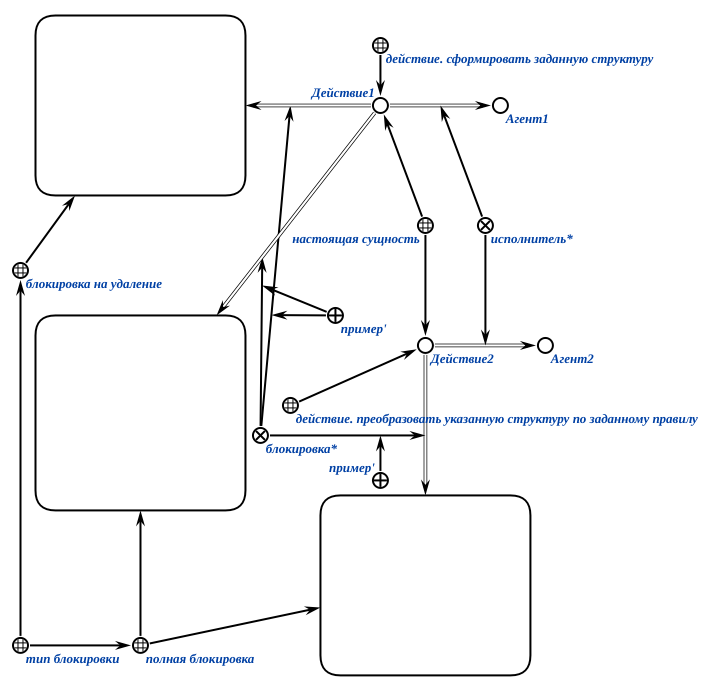
\includegraphics[scale=0.8]{images/part3/chapter_situation_management/lock.png}
	\caption{Пример использования блокировок}
	\label{fig:lock}
\end{figure}

Множество \textbf{\textit{тип блокировки}} содержит все возможные классы блокировок, т.е. \textit{структуры}, содержащие \textit{sc-элементы}, заблокированные каким-либо \textit{sc-агентом} на время выполнения им некоторого \textit{действия в sc-памяти}.

Каждая \textit{структура}, принадлежащая множеству \textbf{\textit{полная блокировка}} содержит \textit{sc-элементы}, просмотр и изменение (удаление, добавление инцидентных \textit{sc-коннекторов}, удаление самих \textit{sc-элементов}, изменение содержимого в случае файла) которых запрещены всем \textit{sc-агентам}, кроме собственно \textit{sc-агента}, выполняющего соответствующее данной структуре \textit{действие в sc-памяти}, связанное с ней отношением \textit{блокировка*}.
	
Для того, чтобы исключить возможность реализации \textit{sc-агентов}, которые могут внести изменения в конструкции, описывающие блокировки других \textit{sc-агентов}, все элементы этих конструкций, в том числе, сам знак \textit{структуры}, содержащей заблокированные \textit{sc-элементы} (принадлежащей как множеству \textbf{\textit{полная блокировка}}, так и любому другому \textit{типу блокировки}) и связки отношения \textit{блокировка*}, связывающие эту \textit{структуру} и конкретное \textit{действие в sc-памяти}, добавляются в \textbf{\textit{полную блокировку}}, соответствующую данному \textit{действию в sc-памяти}. Таким образом, каждой \textbf{\textit{полной блокировке}} соответствует петля принадлежности, связывающая ее знак с самим собой.

Каждая \textit{структура}, принадлежащая множеству \textbf{\textit{блокировка на любое изменение}} содержит \textit{sc-элементы}, изменение (физическое удаление, добавление инцидентных \textit{sc-коннекторов}, физическое удаление самих \textit{\mbox{sc-элементов}}, изменение содержимого в случае файла) которых запрещено всем \textit{sc-агентам}, кроме собственно \textit{sc-агента}, выполняющего соответствующее данной структуре \textit{действие в sc-памяти}, связанное с ней отношением \textit{блокировка*}. Однако не запрещен просмотр (чтение) этих \textit{sc-элементов} любым \textit{sc-агентом}.

Каждая \textit{структура}, принадлежащая множеству \textbf{\textit{блокировка на удаление}} содержит \textit{sc-элементы}, удаление которых запрещено всем \textit{sc-агентам}, кроме собственно \textit{sc-агента}, выполняющего соответствующее данной структуре \textit{действие в sc-памяти}, связанное с ней отношением \textit{блокировка*}. Однако не запрещен просмотр (чтение) этих \textit{sc-элементов} любым \textit{sc-агентом}, добавление инцидентных sc-коннекторов.

Рассмотрим принципы работы с блокировками:

\begin{itemize}
	\item в каждый момент времени одному процессу в sc-памяти может соответствовать только одна блокировка каждого типа;
	\item в каждый момент времени одному процессу в sc-памяти может соответствовать только одна блокировка, установленная на некоторый конкретный sc-элемент;
	\item при завершении выполнения любого процесса в sc-памяти все установленные им блокировки автоматически снимаются;
	\item для повышения эффективности работы системы в целом каждый процесс должен в каждый момент времени блокировать минимально необходимое множество sc-элементов, снимая блокировку с каждого sc-элемента сразу же, как это становится возможным (безопасным);
	\item В случае когда в рамках \textit{процесса в sc-памяти} явно выделяются более частные подпроцессы (при помощи отношений \textit{темпоральная часть*, поддействие*, декомпозиция действия*} и т. д.), то каждый такой подпроцесс с точки зрения синхронизации выполнения рассматривается как самостоятельный процесс, которому в соответствие могут быть поставлены все необходимые блокировки.
	\begin{itemize}
		\item все дочерние процессы в sc-памяти имеют доступ к блокировкам родительского процесса так же, как если бы это были блокировки соответствующие каждому из таких дочерних процессов;
		\item в свою очередь, родительский процесс не имеет какого-либо привилегированного доступа к sc-элементам, заблокированным дочерними процессами, и работает с ними так же, как любой другой процесс в sc-памяти. Исключение составляют sc-элементы, обозначающие сами дочерние процессы, поскольку родительский процесс должен иметь возможность управления дочерним, например, приостановки или прекращения их выполнения;
		\item все дочерние процессы по отношению друг к другу работают так же, как и по отношению к любым другим процессам;
		\item в случае, когда родительский процесс приостанавливает выполнение (становится \textit{отложенным действием}), \uline{все} его дочерние процессы также приостанавливают выполнение. В свою очередь, приостановка одного из дочерних процессов в общем случае не инициирует явно остановку всего родительского процесса и соответственно других дочерних.
		\end{itemize}
\end{itemize}

Рассмотрим принципы работы с \textit{полными блокировками}:
\begin{itemize}
	\item если sc-элемент, инцидентный некоторому sc-коннектору, попадает в какую-либо полную блокировку, то сам этот sc-коннектор по умолчанию также считается заблокированным этой же блокировкой. Обратное в общем случае неверно, т. к. часть sc-коннекторов, инцидентных некоторому sc-элементу, может быть полностью заблокирована, при этом сам этот элемент заблокирован не будет. Такая ситуация типична, например, для sc-узлов, обозначающих классы понятий;
	\item каждый процесс в sc-памяти может свободно изменять или удалять любые sc-элементы, попадающие в полную блокировку, соответствующую этому процессу.
\end{itemize}

Принципы работы с \textit{полными блокировками}, с одной стороны, наиболее просты, поскольку все процессы, кроме установившего такую блокировку, не имеют доступа к заблокированным \mbox{sc-элементам} и конфликты возникнуть не могут. С другой стороны, частое использование блокировок такого типа может привести к тому, что система не сможет использовать в полной мере имеющиеся у нее знания и давать неполные или даже некорректные ответы на поставленные вопросы.

Рассмотрим принципы работы с \textit{блокировками на любое изменение} и \textit{блокировками на удаление}:
\begin{itemize}
	\item на один и тот же sc-элемент в один момент времени может быть установлена только одна блокировка одного типа, но разные процессы могут одновременно установить на один и тот же элемент блокировки двух разных типов. Это касается случая, когда первый процесс установил на некоторый sc-элемент блокировку на удаление, а второй процесс затем устанавливает блокировку на любое изменение. В других случаях возникает конфликт блокировок;
	\item установка блокировки любого типа также считается изменением, таким образом, если на некоторый \mbox{sc-элемент} была установлена блокировка на любое изменение, то другой процесс не сможет установить на этот же sc-элемент блокировку любого типа, пока первый процесс не снимет свою;
	\item если блокировка на удаление устанавливается на некоторый sc-коннектор, то по умолчанию та же блокировка устанавливается на инцидентные этому sc-коннектору sc-элементы, поскольку удаление этих элементов приведет к удалению этого коннектора.
\end{itemize}

\begin{SCn}
\scnheader{процесс в sc-памяти}
\scnidtf{действие в sc-памяти}
\scnrelfrom{разбиение}{Классификация процессов в sc-памяти с точки зрения синхронизации их выполнения}
\begin{scnindent}
\begin{scneqtoset}
	\scnitem{действие поиска sc-элементов}
	\scnitem{действие генерации sc-элементов}
	\scnitem{действие удаления sc-элементов}
	\scnitem{действие установки блокировки некоторого типа на некоторый sc-элемент}
	\scnitem{действие снятия блокировки с некоторого sc-элемента}
\end{scneqtoset}
\end{scnindent}
\end{SCn}

В некоторых случаях для того, чтобы обеспечить синхронизацию, необходимо объединять несколько элементарных действий над sc-памятью в одно неделимое действие (\textbf{\textit{транзакцию в sc-памяти}}), для которого гарантируется, что ни один сторонний процесс не сможет прочитать или изменить участвующие в этом действии sc-элементы, пока действие не завершится. При этом, в отличие от ситуации с полной блокировкой, процесс, пытающийся получить доступ к таким элементам, не продолжает выполнение так, как если бы этих элементов просто не было в sc-памяти, а ожидает завершения транзакции, после чего может выполнять с данными элементами любые действия согласно общим принципам синхронизации процессов. Проблема обеспечения транзакций не может быть решена на уровне SC-кода и требует реализации таких неделимых действий на уровне \textit{платформы интерпретации sc-моделей}.

В случае выполнения \textit{действия поиска sc-элементов} все найденные и сохраненные в рамках какого-либо процесса sc-элементы попадают в соответствующую данному процессу \textit{блокировку на любое изменение}. Таким образом, гарантируется целостность фрагмента базы знаний, с которым работает некоторый процесс в sc-памяти. При этом поиск и автоматическая установка такой блокировки должны быть реализованы как \textit{транзакция в sc-памяти}.
	
Такой подход также позволяет избежать ситуации, когда один процесс заблокировал некоторый sc-элемент на любое изменение, а второй процесс пытается сгенерировать или удалить \textit{sc-коннектор}, инцидентный данному \textit{sc-элементу}. В таком случае второй процесс должен будет предварительно найти и заблокировать указанный \textit{sc-элемент} на любое изменение, что вызовет конфликт блокировок (\textit{взаимоблокировку*}).

В случае генерации любого sc-элемента в рамках некоторого процесса он автоматически попадает в полную блокировку, соответствующую данному процессу. При этом генерация и автоматическая установка такой блокировки должны быть реализованы как \textit{транзакция в sc-памяти}. При необходимости сгенерированные элементы могут быть удалены (т. е. их временное существование вообще никак не отразится на деятельности других процессов) или разблокированы в случае, когда сгенерирована информация, которая может иметь некоторую ценность в дальнейшем.

В случае если какой-либо процесс пытается установить блокировку любого типа на какой-либо sc-элемент, уже заблокированный каким-либо другим процессом, то, с одной стороны, блокировка не может быть установлена, пока другой процесс не разблокирует указанный sc-элемент; с другой стороны, для того чтобы обеспечить возможность поиска и устранения \textit{взаимоблокировок}, необходимо явно указывать тот факт, что какой-либо процесс хочет получить доступ к какому-либо заблокированному другим процессом sc-элементу. Для того чтобы иметь возможность указать, какие процессы пытаются заблокировать уже заблокированный \textit{sc-элемент}, предлагается наряду с отношением \textit{блокировка*} использовать отношение \textit{планируемая блокировка*}, полностью аналогичное отношению \textit{блокировка*}.
	
Описанный механизм регулирует также и процессы поиска, поскольку поиск и сохранение некоторого sc-элемента предполагает установку \textit{блокировки на любое изменение}. Кроме того, следует учитывать, что на один sc-элемент \textit{блокировка на любое изменение} может быть установлена после \textit{блокировки на удаление}, соответствующей другому процессу. В этом случае использовать отношение \textit{планируемые блокировки*} нет необходимости.
	
Действие проверки наличия на некотором sc-элементе блокировки и в зависимости от результата проверки, установки блокировки или планируемой блокировки (с указанием приоритета при необходимости) должно быть реализовано как транзакция.

\begin{SCn}
\scnheader{планируемая блокировка*}
\scnsubset{блокировка*}
\end{SCn}

Процесс, которому в соответствие поставлена \textit{планируемая блокировка*}, приостанавливает выполнение до тех пор, пока уже установленные блокировки не будут сняты, после чего \textit{планируемая блокировка*} становится реальной \textit{блокировкой*} и процесс продолжает выполнение в соответствии с общими правилами.

\begin{SCn}
\scnheader{приоритет блокировки*}
\scnrelfrom{область определения}{планируемая блокировка*}
\end{SCn}

В случае, когда на один и тот же sc-элемент планируют установить блокировку сразу несколько процессов, используется отношение \textit{приоритет блокировки*}, связывающее между собой пары отношения \textit{планируемая блокировка*}. Как правило, приоритет блокировки определяется тем, какой из процессов раньше попытался установить блокировку на рассматриваемый sc-элемент, хотя в общем случае приоритет может устанавливаться или меняться в зависимости от дополнительных критериев.

В случае попытки удаления некоторого sc-элемента некоторым процессом удаление может быть осуществлено только в случае, когда на данный sc-элемент не установлена (и не планируется) ни одна блокировка каким-либо другим процессом.
	
В других случаях необходимо обеспечить корректное завершение выполнения всех процессов, работающих с данным sc-элементом, и только потом удалить его физически.
	
Для реализации такой возможности каждому процессу в соответствие может быть поставлено множество удаляемых данным процессом sc-элементов.

Действие проверки наличия блокировок или планируемых блокировок на удаляемый sc-элемент и собственно его удаление или добавление во множество удаляемых sc-элементов для соответствующего процесса должно быть реализовано как транзакция.

\begin{SCn}
\scnheader{удаляемые sc-элементы*}
\scnrelfrom{первый домен}{процесс в sc-памяти}
\end{SCn}

Sc-элементы, попавшие во множество удаляемых sc-элементов некоторого процесса в sc-памяти, доступны процессам, уже установившим (или планирующим установить) на эти sc-элементы блокировки ранее (до попытки его удаления), а для всех остальных процессов эти sc-элементы уже считаются удаленными. Процесс, пытающийся удалить sc-элемент, приостанавливает свое выполнение до того момента, пока все заблокировавшие и планирующие заблокировать данный sc-элемент процессы не разблокируют его. В общем случае один sc-элемент может входить во множества удаляемых элементов одновременно для нескольких процессов, в этом случае все такие процессы одновременно продолжат выполнение после снятия с этого sc-элемента всех блокировок. Если удаление пытается осуществить один из процессов, уже установивший на указанный sc-элемент блокировку, то алгоритм действий остается прежним -- sc-элемент добавляется во множество удаляемых данным процессом sc-элементов, и будет физически удален, как только все остальные процессы, установившие на данный sc-элемент блокировки, снимут их.

Рассмотрим алгоритм снятия блокировки с некоторого sc-элемента:
\begin{enumerate}
	\item если на данный sc-элемент установлена одна или несколько \textit{планируемых блокировок*}, то первая из них по приоритету (или единственная) становится \textit{блокировкой*}, соответствующий ей процесс продолжает выполнение (становится настоящей сущностью); связка отношения приоритет выполнения, соответствовавшая удаленной связке отношения \textit{планируемая блокировка*} также удаляется, т. е. приоритет смещается на одну позицию;
	\item если \textit{планируемых блокировок*}, установленных на данный sc-элемент, нет, но он попадает во множество удаляемых sc-элементов для одного или нескольких процессов, то рассматриваемый sc-элемент физически удаляется, а приостановленные до его удаления процессы продолжают свое выполнение (становится настоящими сущностями);
	\item если на данный sc-элемент не установлены планируемые блокировки и он не входит во множество удаляемых для какого-либо процесса, то блокировка просто снимается без каких-либо дополнительных изменений.
\end{enumerate}

\begin{SCn}
\scnheader{транзакция в sc-памяти}
\begin{scnrelfromset}{разбиение}
	\scnitem{поиск некоторой конструкции в sc-памяти и автоматическая установка блокировки на любое изменение на найденные sc-элементы}
	\scnitem{генерация некоторого sc-элемента и автоматическая установка на него полной блокировки}
	\scnitem{проверка наличия на некотором sc-элементе блокировки и в зависимости от результата проверки установка блокировки или планируемой блокировки}	
	\scnitem{проверка наличия блокировок или планируемых блокировок на удаляемый sc-элемент и собственно его удаление или добавление во множество удаляемых sc-элементов для соответствующего процесса}	
	\scnitem{снятие блокировки с заданного sc-элемента и при необходимости установка первой по приоритету планируемой блокировки или удаление данного sc-элемента, если он входит во множество удаляемых sc-элементов для некоторого процесса}	
	\scnitem{поиск подпроцессов процесса и добавление их во множество отложенных действий в случае добавления самого процесса в данное множество}	
	\scnitem{поиск подпроцессов процесса и удаление их из множества отложенных действий в случае удаления самого процесса из данного множества}	
\end{scnrelfromset}
\end{SCn}

При реализации \textit{абстрактных программных sc-агентов} на \textit{языке SCP}, соблюдение всех принципов синхронизации соответствующих этим sc-агентам процессов обеспечивается на уровне \textit{sc-агентов интерпретации scp-программ}, т. е. средствами \textit{платформы интерпретации sc-моделей}. При реализации \textit{абстрактных программных sc-агентов} на уровне платформы, соблюдение всех принципов синхронизации возлагается, во-первых, непосредственно на разработчика агентов, во-вторых, -- на разработчика платформы. Так, например, платформа может предоставлять доступ к хранимым в sc-памяти элементам через некоторый программный интерфейс, уже учитывающий принципы работы с блокировками, что избавит разработчика агентов от необходимости учитывать все эти принципы вручную.

Кроме того, выделяется ряд специфичных принципов работы \textit{абстрактных программных sc-агентов}, реализованных на \textit{языке SCP}:
\begin{itemize}
\item в результате появления в sc-памяти некоторой конструкции, удовлетворяющей условию инициирования какого-либо \textit{абстрактного sc-агента}, реализованного при помощи \textit{Языка SCP}, в \textit{sc-памяти} генерируется и инициируется \textit{scp-процесс}. В качестве шаблона для генерации используется \textit{агентная scp-программа}, соответствующая данному \textit{абстрактному sc-агенту}.
\item каждый такой \textit{scp-процесс}, соответствующий некоторой \textit{агентной \mbox{scp-программе}}, может быть связан с набором структур, описывающих блокировки различных типов. Таким образом, синхронизация взаимодействия параллельно выполняемых \textit{scp-процесcов} осуществляется так же, как и в случае любых других \textit{действий в sc-памяти}.
\item несмотря на то что каждый \textit{scp-оператор} представляет собой атомарное действие в sc-памяти, являющееся поддействием в рамках всего \textit{\mbox{scp-процесса}}, блокировки, соответствующие одному оператору, не вводятся, чтобы избежать громоздкости и избытка дополнительных системных конструкций, создаваемых при выполнении некоторого \textit{scp-процесса}. Вместо этого используются блокировки, общие для всего \textit{scp-процесса}. Таким образом, \textit{агенты интерпретации scp-программ} работают только с учетом блокировок, общих для всего интерпретируемого \textit{scp-процесса}.
\item процессы, описывающие деятельность агентов интерпретации \textit{scp-программ}, как правило, не создаются, следовательно, и не вводятся соответствующие им блокировки. Поскольку такие агенты работают с уникальным scp-процессом и их число ограничено и известно, то использование блокировок для их синхронизации не требуется.
\item в случае приостановки \textit{scp-процесса} (добавления его во множество \textit{отложенных действий}) в соответствии с общими правилами синхронизации все его дочерние процессы также должны быть	приостановлены. В связи с этим все \textit{scp-операторы}, которые в	этот момент являются \textit{настоящими сущностями}, становятся	\textit{отложенными действиями}.
\item во избежание нежелательных изменений в самом теле \textit{scp-процесса}, вся конструкция, сгенерированная на основе некоторой \textit{scp-программы} (весь \textit{sc-текст}, описывающий декомпозицию \textit{scp-процесса} на \textit{scp-операторы}), должна быть добавлена в \textit{полную блокировку}, соответствующую данному \textit{scp-процессу}.
\item при необходимости разблокировать или заблокировать некоторую конструкцию каким-либо типом блокировки используются соответствующие \textit{scp-операторы} класса \textit{scp-оператор управления блокировками}.
\item после завершения выполнения некоторого scp-процесса его текст, как правило, удаляется из \textit{sc-памяти}, а все заблокированные конструкции освобождаются (разрушаются знаки структур, обозначавших блокировки).
\item как правило, частный \textit{класс действий}, соответствующий конкретной \textit{scp-программе}, явно не вводится, а используется более общий класс \textit{scp-процесс}, за исключением тех случаев, когда введение	специального \textit{класса действий} необходимо по каким-либо другим соображениям.
\end{itemize}

В общем случае весь механизм блокировок может описываться как на уровне SC-кода (для повышения уровня платформенной независимости), так и при необходимости может быть реализован на уровне \textit{платформы интерпретации sc-моделей}, например для повышения производительности. Для этого каждому выполняемому в sc-памяти процессу на нижнем уровне может быть поставлена в соответствие некая уникальная таблица, в каждый момент времени содержащая перечень заблокированных элементов с указанием типа блокировки.

Рассмотрим пример применения описанного механизма.

\begin{figure}[h]
	\centering
	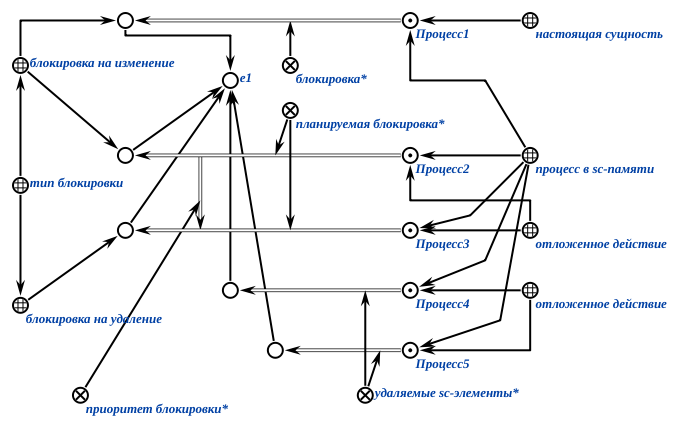
\includegraphics[scale=0.8]{images/part3/chapter_situation_management/plan_lock_1.png}
	\caption{Пример использования планируемых блокировок}
	\label{fig:plan_lock_1}
\end{figure}

В данном примере \textit{Процесс1} непосредственно работает с sc-элементом \textit{\textbf{e1}},\textit{Процесс2} и \textit{Процесс3} планируют установить блокировку на любое изменение и блокировку на удаление соответственно, причем \textit{Процесс2} попытался установить свою блокировку раньше, чем \textit{Процесс3}, поэтому согласно направлению связки отношения \textit{приоритет блокировки*}, его блокировка будет установлена раньше. \textit{Процесс4} и \textit{Процесс5} ожидают снятия всех блокировок и планируемых блокировок, после чего \textit{\textbf{e1}} будет удален и \textit{Процесс1} и \textit{Процесс2} продолжат свое выполнение. Никакие другие планируемые блокировки установлены быть уже не могут, поскольку \textit{\textbf{e1}} попал во множество удаляемых sc-элементов как минимум одного процесса и, в соответствии с изложеннымивыше правилами, все остальные процессы кроме \textit{Процесс1}-\textit{Процесс5}, уже несмогут получить доступ к этому sc-элементу.		
Выполняемый процесс принадлежит множеству настоящая сущность, приостановленные -- множеству отложенное действие.

\begin{figure}[h]
	\centering
	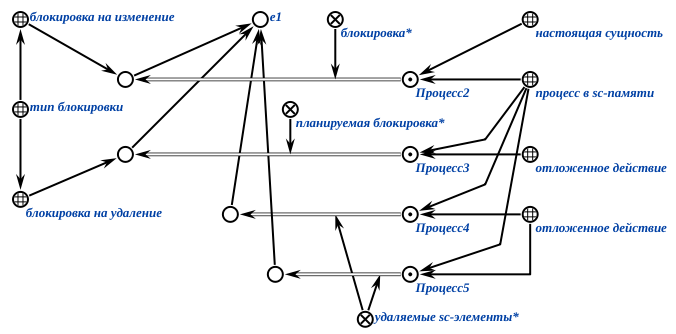
\includegraphics[scale=0.8]{images/part3/chapter_situation_management/plan_lock_2.png}
	\caption{Пример использования планируемых блокировок (продолжение)}
	\label{fig:plan_lock_2}
\end{figure}

После того как \textit{Процесс1} разблокировал sc-элемент \textit{\textbf{e1}}, этот элемент будет заблокирован \textit{Процессом2}, и \textit{Процесс2} продолжит выполнение. \textit{Планируемая блокировка*}, установленная \textit{Процессом2}, становится обычной \textit{блокировкой*}.

\begin{figure}[h]
	\centering
	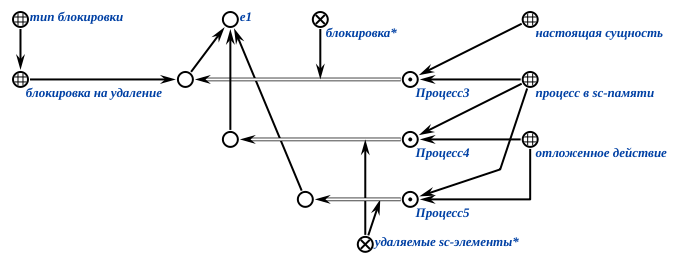
\includegraphics[scale=0.8]{images/part3/chapter_situation_management/plan_lock_3.png}
	\caption{Пример использования блокировки на удаление}
	\label{fig:plan_lock_3}
\end{figure}

После того как \textit{Процесс2} разблокировал sc-элемент \textit{\textbf{e1}}, этот элемент будет заблокирован \textit{Процессом3}, и \textit{Процесс3} продолжит выполнение.

\begin{figure}[h]
	\centering
	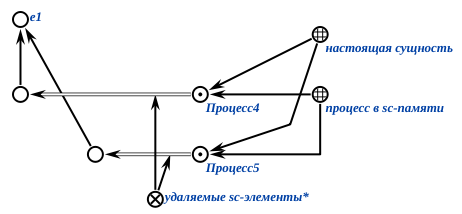
\includegraphics[scale=0.8]{images/part3/chapter_situation_management/plan_lock_4.png}
	\caption{Удаляемые sc-элементы}
	\label{fig:plan_lock_4}
\end{figure}

Когда все процессы снимут блокировки с sc-элемента \textit{\textbf{e1}}, он может быть физически удален и \textit{Процесс4} и \textit{Процесс5} продолжат выполнение.

В зависимости от конкретных \textit{типов блокировок} установленных паралельно выполняемыми процессами на некоторые sc-элементы и того, какие конкретно действия с этими \textit{sc-элементами} предполагается выполнить далее в рамках выполнения этих процессов, возможны ситуации взаимоблокировки, когда каждый из указанных процессов будет ожидать снятия блокировки вторым процессом с нужного \textit{sc-элемента}, не снимая при этом установленной им самим блокировки с \textit{sc-элемента}, доступ к которому необходим второму процессу.
	
В случае когда хотя бы одна из блокировок является \textit{полной блокировкой}, ситуация взаимоблокировки возникнуть не может, поскольку \textit{sc-элементы}, попавшие в \textit{полную блокировку} некоторого \textit{scp-процесса}, не доступны другим \textit{scp-процессам} даже для чтения и, таким образом, остальные \textit{scp-процессы} будут работать так, как будто заблокированные \textit{sc-элементы} просто отсутствуют в текущем состоянии \textit{sc-памяти}.

В случаях, когда ни одна из установленных блокировок не является \textit{полной блокировкой}, возможно появление взаимоблокировок.

Устранение \textit{взаимоблокировки} невозможно без вмешательства специализированного \textit{sc-метаагента}, который имеет право игнорировать блокировки, установленные другими процессами. 
	
В общем случае проблема конкретной взаимоблокировки может быть решена путем выполнения специализированным \textit{sc-метаагентом} следующих шагов:	
\begin{itemize}
	\item откат нескольких операций, выполненных одним из участвующих в взаимоблокировке процессов настолько шагов назад, насколько это необходимо для того, чтобы второй процесс получил доступ к необходимым \textit{sc-элементам} и смог продолжить выполнение;
	\item ожидание выполнения второго процесса вплоть до завершения или до снятия им всех блокировок с \textit{sc-элементов}, доступ к которым необходимо получить первому процессу;
	\item повторное выполнение в рамках первого процесса отмененных операций и продолжение его выполнения, но уже с учетом изменений в памяти, внесенных вторым процессом.		
\end{itemize}

Для \textit{sc-метаагентов} все sc-элементы, в том числе описывающие блокировки, планируемые блокировки и т. д. полностью эквивалентны между собой с точки зрения доступа к ним, т. е. любой \textit{sc-метаагент} имеет доступ к любым sc-элементам, даже попавшим в полную блокировку для какого-либо другого процесса. Это необходимо для того, чтобы \textit{sc-метаагенты} смогли выявлять и устранять различные проблемы, например, описанную выше проблему взаимоблокировки.

Таким образом, проблема синхронизации деятельности \textit{sc-метаагентов} требует введения дополнительных правил.

Указанную проблему разделим на две более частные:
\begin{itemize}
	\item обеспечение синхронизации деятельности \textit{sc-метаагентов} между собой;
	\item обеспечение синхронизации деятельности \textit{sc-метаагентов} и \textit{программных sc-агентов}.		
\end{itemize}

Первую проблему предлагается решить за счет запрета параллельного выполнения \textit{sc-метаагентов}. Таким образом, в каждый момент времени в рамках одной \textit{ostis-системы} может существовать только один процесс, соответствующий \textit{sc-метаагенту} и являющийся \textit{настоящей сущностью}. 

Вторую проблему предлагается решить за счет введения дополнительных привилегий для \textit{sc-метаагентов} при обращении к какому-либо sc-элементу. Для этого достаточно одного правила: 

Если некоторый sc-элемент стал использоваться в рамках процесса, соответствующего \textit{sc-метаагенту} (например, стал элементом хотя бы одного scp-оператора, входящего в данный процесс), то все процессы, в блокировки соответствующие которым попадает указанный sc-элемент, становятся отложенными действиями (приостанавливают выполнение). Как только указанный sc-элемент перестает использоваться в рамках процесса, соответствующего \textit{sc-метаагенту}, все приостановленные по этой причине процессы продолжают выполнение.

Рассмотренные ограничения не ухудшают производительность ostis-системы существенно, поскольку \textit{sc-метаагенты} предназначены для решения достаточно узкого класса задач, которые, как показал опыт практической разработки прототипов различных \textit{ostis-систем}, возникают достаточно редко.
	
Стоит отметить, что возможна ситуация, при которой выполнение некоторого процесса в sc-памяти прервано по причине возникновения какой-либо ошибки. В таком случае существует вероятность того, что блокировка, установленная данным процессом не будет снята до тех пор, пока этого не сделает sc-метаагент, обнаруживший подобную ситуацию. Однако указанная проблема на уровне sc-модели может быть решена лишь частично, для случаев, когда ошибка возникает при интерпретации scp-программы, отслеживается scp-интепретатором и в памяти формируется соответствующая конструкция, сообщающая о проблеме sc-метаагенту. Случаи, когда возникла ошибка на уровне scp-интерпретатора или sc-хранилища, должны рассматриваться на уровне платформы интерпретации sc-моделей.

\section{Базовый язык программирования ostis-систем}
\subsection{Синтаксис Базового языка программирования ostis-систем}
\subsection{Денотационная семантика Базового языка программирования ostis-систем}
\subsection{Операционная семантика Базового языка программирования ostis-систем}

%\input{author/references}
\chapter{Язык вопросов для ostis-систем}
\chapauthortoc{Самодумкин С.~А.\\Зотов Н.~В.\\Шункевич Д.~В.\\ Ивашенко В.~П.}
\label{chapter_requests}

\vspace{-7\baselineskip}

\begin{SCn}
\begin{scnrelfromlist}{авторы}
	\scnitem{Самодумкин С.~А.}
	\scnitem{Зотов Н.~В.}
	\scnitem{Шункевич Д.~В.}
	\scnitem{Ивашенко В.~П.}
\end{scnrelfromlist}

\bigskip

\scntext{аннотация}{Возможности \textit{баз знаний} \textit{ostis-систем} позволяют не только представлять и структурировать знания об окружающем мире, но и быстро получать и формировать эти знания о нем, тем самым удовлетворяя информационную потребность пользователя. В данной главе уточнена формальная спецификация \textit{Языка вопросов для ostis-систем}, позволяющая описывать и интерпретировать любые классы \textit{вопросов} \textit{пользователей ostis-систем}.}

\bigskip

\begin{scnrelfromlist}{подраздел}
	\scnitem{\ref{sec_requests_syntax}~\nameref{sec_requests_syntax}}
	\scnitem{\ref{sec_requests_den_semantics}~\nameref{sec_requests_den_semantics}}
	\scnitem{\ref{sec_requests_op_semantics}~\nameref{sec_requests_op_semantics}}
\end{scnrelfromlist}

\bigskip

\begin{scnrelfromlist}{ключевое понятие}
	\scnitem{вопрос}
	\scnitem{ответ на вопрос}
	\scnitem{знак в рамках заданного вопроса}
	\scnitem{основной знак в рамках заданного вопроса}
	\scnitem{неосновной знак в рамках заданного вопроса}
	\scnitem{отношение в рамках заданного вопроса}
	\scnitem{базовое отношение в рамках заданного вопроса}
	\scnitem{интерпретатор Языка вопросов для ostis-систем}
\end{scnrelfromlist}

\begin{scnrelfromlist}{ключевой знак}
	\scnitem{Язык вопросов для ostis-систем}
	\scnitem{Синтаксис Языка вопросов для ostis-систем}
	\scnitem{Денотационная семантика Языка вопросов для ostis-систем}
	\scnitem{Семантическая классификация вопросов}
	\scnitem{Операционная семантика Языка вопросов для ostis-систем}
\end{scnrelfromlist}

\bigskip

\begin{scnrelfromlist}{библиографическая ссылка}
	\scnitem{\scncite{Averyanov1993}}
	\scnitem{\scncite{Suleimanov2001}}
	\scnitem{\scncite{Suleimanov2014}}
	\scnitem{\scncite{Bukharev1990}}
	\scnitem{\scncite{Kwok2001}}
	\scnitem{\scncite{Emelyanov2007}}
	\scnitem{\scncite{Finn1976}}
	\scnitem{\scncite{Finn1981}}
	\scnitem{\scncite{Belnap1981}}
	\scnitem{\scncite{Sosnin2007}}
	\scnitem{\scncite{Zaharov2002}}
	\scnitem{\scncite{Hant1978}}
	\scnitem{\scncite{Lyubarsky1990}}
	\scnitem{\scncite{Samodumkin2009}}
	\scnitem{\scncite{Samodumkin2009a}}
\end{scnrelfromlist}
	
\end{SCn}

\section*{Введение в Главу \ref{chapter_requests}}

Одна из ключевых особенностей \textit{интеллектуальной системы} состоит в том, что \textit{пользователь} имеет возможность формулировать свою информационную потребность. Cпособом выражения такой потребности является \textit{вопрос}. В процессе общения всегда существует контекст, который определяет дополнительную информацию, способствующую правильному пониманию \textit{смысла} сообщения. Особенность представления информации в \textit{базах знаний} \textit{ostis-систем} упрощает формирование информационной потребности пользователя, так как представленная информация в \textit{базах знаний} уже структурирована и известны отношения, заданные на определенном понятии, в отношении которого разрешается вопросно-проблемная ситуация. В работе \scncite{Averyanov1993} показано, что вопросно-проблемная ситуация не может быть решена в рамках формальной логики и природа вопроса может быть понятна в системе субъектно-объектных отношений. В связи с тем, что при формировании \textit{баз знаний} \textit{ostis-систем} происходит формирование субъектно-объектных отношений в рамках заданной \textit{предметной области}, тем самым упрощается выражение информационной потребности пользователем средствами \textit{SC-кода}.   

Целью разработки \textbf{\textit{Языка вопросов для ostis-систем}} и последующего его развития является реализация возможности понимания действий, осуществляемых \textit{ostis-системой}, при формировании ответа на поставленный \textit{вопрос}. В процессе формирования ответа на поставленный \textit{вопрос} возможны следующие варианты:
\begin{textitemize}
	\item \textit{ответ на} поставленный \textit{вопрос} существует в \textit{базе знаний} и происходит локализация \textit{фрагмента базы знаний} в контексте выраженной средствами \textit{SC-кода} информационной потребности \textit{пользователя};
	\item ответ связан с разрешением некоторой задачной ситуации, которая содержится в контексте \textit{вопроса} и формирование \textit{ответа на вопрос} возлагается на \textit{решатель задач} (см. \textit{Главу \ref{chapter_situation_management}~\nameref{chapter_situation_management}}).
\end{textitemize}

\begin{SCn}
\scnheader{Язык вопросов для ostis-систем}
\scnidtf{Предлагаемый нами вариант языка для описания вопросов и ответов на них в ostis-системах}
\scniselement{sc-язык}
\scnrelfrom{синтаксис языка}{Синтаксис Языка вопросов для ostis-систем}
\begin{scnindent}
	\scnsubset{Синтаксис SC-кода}
\end{scnindent}
\scnrelfrom{денотационная семантика языка}{Денотационная семантика Языка вопросов для ostis-систем}
\begin{scnindent}
	\scnidtf{Онтология классов знаков и отношений для описания формулировок вопросов на SC-коде}
	\scnsuperset{Семантическая классификация вопросов}
\end{scnindent}
\scnrelfrom{операционная семантика языка}{Операционная семантика Языка вопросов для ostis-систем}
\begin{scnindent}
	\scnidtf{Коллектив sc-агентов вывода ответов на заданные вопросы пользователя ostis-системы}
\end{scnindent}
\end{SCn}

\section{Синтаксис Языка вопросов для ostis-систем}
\label{sec_requests_syntax}

\textit{Язык вопросов для ostis-систем} относится к семейству семантических совместимых языков --- \textit{sc-языков} и предназначен для формального описания поискового предписания \textit{ostis-систем} с целью удовлетворения информационной потребности \textit{пользователя}. Поэтому \textbf{\textit{Синтаксис Языка вопросов для ostis-систем}}, как и \textit{синтаксис} любого другого \textit{sc-языка}, является \textit{Синтаксисом SC-кода}. Такой подход позволяет:
\begin{textitemize}
	\item унифицировать форму представления \textit{вопросов} и \textit{знаний}, с помощью которых строятся ответы на поставленные \textit{вопросы};
	\item использовать минимум средств для интерпретации заданных \textit{вопросов пользователей};
	\item сводить формирование ответов на большую часть заданных \textit{вопросов} к поиску информации в текущем состоянии \textit{базы знаний ostis-системы}.
\end{textitemize}

\section{Денотационная семантика Языка вопросов для ostis-систем}
\label{sec_requests_den_semantics}

\begin{SCn}
\begin{scnrelfromlist}{ключевое понятие}
	\scnitem{вопрос}
	\scnitem{ответ на вопрос}
	\scnitem{знак в рамках заданного вопроса}
	\scnitem{основной знак в рамках заданного вопроса}
	\scnitem{неосновной знак в рамках заданного вопроса}
	\scnitem{отношение в рамках заданного вопроса}
	\scnitem{базовое отношение в рамках заданного вопроса}
\end{scnrelfromlist}
\end{SCn}

\textbf{\textit{Денотационная семантика Языка вопросов для ostis-систем}} включает \textit{классы вопросов} и соответствующие \textit{классы ответов}, необходимые для спецификации формулировок \textit{вопросов} и \textit{ответов} на них, а также \textit{классы знаков} и \textit{отношений}, входящих в структуру любого \textit{вопроса}. В \textit{Семантической классификации вопросов} \textit{Языка вопросов для ostis-систем} заложена идея, описанная в работе \scncite{Suleimanov2001}.

Любой \textbf{\textit{вопрос}} на \textit{Языке вопросов для ostis-систем} представляет собой \textit{спецификацию действия} на поиск или синтез \textit{знания}, удовлетворяющего информационную потребность \textit{пользователя}, инициирующего этот \textit{вопрос}. То есть \textit{вопрос} --- это ничто иное как \textit{задача}, с помощью которой выражается потребность пользователя в некоторой информации, возможно хранимой или выводимой в \textit{базе знаний} \textit{ostis-системы} (см. \textit{Главу \ref{chapter_actions}~\nameref{chapter_actions}}). 

Каждому \textit{вопросу} можно взаимно однозначно сопоставить некоторое множество \textit{ответов на} этот \textit{вопрос}. Каждый \textit{ответ на вопрос} представляет собой некоторую \textit{sс-структуру} \textit{семантической окрестности основного знака}, раскрываемого в этом \textit{ответе на} заданный \textit{вопрос}.

\begin{SCn}
\scnheader{вопрос}
\scnidtf{запрос}
\scnidtf{непроцедурная формулировка задачи на поиск (в текущем состоянии базы знаний) или на синтез знания, удовлетворяющего заданным требованиям}
\scnidtf{запрос метода (способа) решения заданного (указываемого) \textit{класса задач} либо \textit{плана решения} конкретной указываемой \textit{задачи}}
\scnidtf{задача, направленная на удовлетворение информационной потребности некоторого субъекта-заказчика}
\scnsubset{задача}

\scnheader{ответ на вопрос}
\scnidtf{ответ на запрос}
\scnidtf{результат запроса}
\scnidtf{результат решения задачи на поиск или синтез знания, удовлетворяющий заданным требованиям}
\scnidtf{семантическая окрестность \textit{основного знака}, знание в которой удовлетворяет информационную потребность пользователя}
\scnidtf{знание в базе знаний ostis-системы, которое удовлетворяет информационную потребность пользователя}
\scnsubset{знание}
\end{SCn}

Среди всех классов \textit{знаков в рамках заданного вопроса} \textit{Языка вопросов для ostis-систем} можно выделить наиболее общие по иерархии классы \textit{знаков}:

\begin{SCn}
\scnheader{знак в рамках заданного вопроса}
\scnsubset{знак}
\begin{scnrelfromset}{разбиение}
	\scnitem{основной знак в рамках заданного вопроса}
	\begin{scnindent}
		\scnidtf{ключевой sc-элемент в рамках заданного вопроса}
		\scnidtf{\textit{знак}, относительно которого задан вопрос}
	\end{scnindent}
	\scnitem{неосновной знак в рамках заданного вопроса}
	\begin{scnindent}
		\scnidtf{\textit{знак}, стоящий в некотором отношении с \textit{основным знаком в рамках заданного вопроса}}
	\end{scnindent}
\end{scnrelfromset}
\end{SCn}

\textbf{\textit{знаком в рамках заданного вопроса}} является любой \textit{знак понятия} или \textit{сущности}, принадлежащий этому \textit{вопросу}. Между \textit{знаками в рамках заданного вопроса} задается множество связей \textit{отношений}, входящих в состав различных \textit{предметных областей}. Кроме того, любое \textbf{\textit{отношение в рамках заданного вопроса}} представляет собой \textit{отношение} между \textit{знаками} \textit{предметной области}, принадлежащих заданному \textit{вопросу}. Среди всех классов \textit{отношений в рамках заданного вопроса} можно выделить класс \textbf{\textit{базовых отношений в рамках заданного вопроса}} и класс \textbf{\textit{составных отношений в рамках заданного вопроса}}.

\begin{SCn}
\scnheader{отношение в рамках заданного вопроса}
\scnidtf{определенное отношение между знаками \textit{предметной области} в контексте \textit{вопроса}}
\scnsubset{отношение}

\scnheader{базовое отношение в рамках заданного вопроса}
\scnidtf{\textit{класс отношений}, объединяющий \textit{отношения в заданном вопросе}, отражающие однотипный \textit{смысл} и раскрывающие определенный признак \textit{знаков} \textit{предметной области}}
\scnsubset{отношение в рамках заданного вопроса}
\begin{scnrelfromset}{декомпозиция}
	\scnitem{отношение состояния}
	\scnitem{отношение действия}
	\scnitem{отношение состава}
	\scnitem{теоретико-множественное отношение}
	\scnitem{темпоральное отношение}
	\scnitem{пространственное отношение}
	\scnitem{количественное отношение}
	\scnitem{качественное отношение}
\end{scnrelfromset}
\end{SCn}

Например, \textit{отношения в рамках заданного вопроса} такие, как \scnqqi{играет*}, \scnqqi{спит*}, \scnqqi{плавает*}, объединяются в класс \textit{отношений состояния} по признаку выражать состояние знака (то есть данные отношения раскрывают признак \textit{знака} \textit{предметной области} --- \scnqqi{находиться в некотором состоянии}).

\begin{SCn}
\scnheader{составное отношение в рамках заданного вопроса}
\scnidtf{устойчивая комбинация двух \textit{отношений действия}: действия, направленного на \textit{параметр вопроса\scnrolesign}, и действия, направленного на \textit{ответ на вопрос*}}
\end{SCn}

Например, элемент \textit{составного отношения в рамках заданного вопроса} между \textit{знаками}: \scnqqi{\textit{Нефтеперерабатывающий завод}}, \scnqqi{\textit{нефть}} и \scnqqi{\textit{нефтепродукты}} --- может быть представлен как \scnqqi{Нефтеперерабатывающий завод перерабатывает нефть в нефтепродукты}.

Смысловая классификация \textit{вопросов} дает возможность противопоставить каждому типу вопроса ограниченный набор допустимых, то есть \textit{семантически корректных информационных конструкций}, передающий правильный \textit{смысл} \textit{вопроса} в зависимости от класса \textit{вопроса}. При этом \textbf{\textit{Семантическая классификация вопросов}} позволяет разбить множество \textit{вопросов} на классы, в каждом из которых требуется раскрытие некоторого однотипного \textit{смысла}, заданного классом этого \textit{вопроса}. 

\begin{SCn}
\scnheader{вопрос}
\begin{scnrelfromset}{декомпозиция}
	\scnitem{вопрос, требующий вывода семантической окрестности \textit{основного знака}}
	\begin{scnindent}
		\begin{scnhaselementrolelist}{пример}
			\scnitem{Вопрос. Что такое \textit{Город Минск}}
		\end{scnhaselementrolelist}
	\end{scnindent}
	\scnitem{вопрос, требующий раскрытия в ответе \textit{базового отношения} \textit{основного знака}}
	\begin{scnindent}
		\begin{scnhaselementrolelist}{пример}
			\scnitem{Вопрос. Что легче: железо или дерево}
		\end{scnhaselementrolelist}
	\end{scnindent}
	\scnitem{вопрос, требующий раскрытия в ответе \textit{составного отношения} \textit{основного знака}}
	\begin{scnindent}
		\scntext{пояснение}{Такому классу \textit{вопросов} соответствуют классы \textit{ответов}, в которых \textit{главный знак} раскрывается через \textit{составное отношение}.}
		\begin{scnhaselementrolelist}{пример}
			\scnitem{Вопрос. Какие Принципы компонентного проектирования в интеллектуальных компьютерных системах нового поколения}
		\end{scnhaselementrolelist}
	\end{scnindent}
	\scnitem{вопрос, требующий раскрытия в ответе произвольной комбинации \textit{базового отношения} и/или \textit{составного отношения} \textit{основного знака}}
	\begin{scnindent}
		\begin{scnhaselementrolelist}{пример}
			\scnitem{Вопрос. Как определяется уровень интеллекта кибернетической системы}
		\end{scnhaselementrolelist}
	\end{scnindent}
	\scnitem{вопрос, требующий раскрытия в ответе более чем одного \textit{основного знака}}
	\begin{scnindent}
		\begin{scnhaselementrolelist}{пример}
			\scnitem{Вопрос. Докажите теорему Пифагора}
		\end{scnhaselementrolelist}
	\end{scnindent}
\end{scnrelfromset}
\end{SCn}

\begin{SCn}
\scnheader{вопрос, требующий раскрытия в ответе \textit{базового отношения} \textit{основного знака}}
\begin{scnrelfromset}{декомпозиция}
	\scnitem{вопрос, требующий раскрытия в ответе \textit{отношения состава} \textit{основного знака}}
	\begin{scnindent}
		\scnidtf{класс вопросов, в ответах на которые \textit{основной знак} \textit{S} раскрывается через его \textit{отношение состава} в связке с его составляющими знаками \textit{P} и \textit{Q}}
		\begin{scnhaselementrolelist}{пример}
			\scnitem{Вопрос. Какие административные районы входят в состав Города Витебск}
			\begin{scnindent}
				\scneqimage[30em]{author/part3/figures/question\_about\_vitebsk\_regions.png}
				\scnrelfrom{ответ на вопрос}{\{Железнодорожный район Города Витебск, Октябрьский район Города Витебск, Первомайский район Города Витебск\}}
				\begin{scnindent}
					\scneqimage[30em]{author/part3/figures/question\_about\_vitebsk\_regions\_answer.png}
				\end{scnindent}
			\end{scnindent}
		\end{scnhaselementrolelist}
	\end{scnindent}
	\scnitem{вопрос, требующий раскрытия в ответе \textit{теоретико-множественного отношения} \textit{основного знака}}
	\begin{scnindent}
		\scnidtf{класс вопросов, в ответах на которые \textit{основной знак} \textit{S} раскрывается через его \textit{теоретико-множественное отношение} в связке с другим знаком \textit{P}, содержащего \textit{S} как часть}
		\begin{scnhaselementrolelist}{пример}
			\scnitem{Вопрос. Частью какой области является Смолевичский район}
			\begin{scnindent}
				\scneqimage[30em]{author/part3/figures/question\_about\_smolevichi\_inclusion.png}
				\scnrelfrom{ответ на вопрос}{\{Смолевичский район является частью Минской области\}}
			\end{scnindent}
		\end{scnhaselementrolelist}
	\end{scnindent}
	\scnitem{вопрос, требующий раскрытия в ответе \textit{отношения состояния} \textit{основного знака}}
	\begin{scnindent}
		\scnidtf{класс вопросов, в ответах на которые \textit{основной знак} \textit{S} раскрывается через его \textit{отношение состояния}}
		\begin{scnhaselementrolelist}{пример}
			\scnitem{Вопрос. Какие города современной территории Республики Беларусь имели Магдебургское право}
			\begin{scnindent}
				\scneqimage[30em]{author/part3/figures/question\_about\_minsk\_district\_town\_with\_mag\_act.png}
				\scnrelfrom{ответ на вопрос}{\{Волковыск, Гродно, Мозырь и другие имели Магдебургское право\}}
			\end{scnindent}
		\end{scnhaselementrolelist}
	\end{scnindent}
	\scnitem{вопрос, требующий раскрытия в ответе \textit{отношения действия} \textit{основного знака}}
	\begin{scnindent}
		\scnidtf{класс вопросов, в ответах на которые \textit{основной знак} \textit{S} раскрывается через его \textit{отношение действия} в связке с другим знаком \textit{P}}
	\end{scnindent}
	\scnitem{вопрос, требующий раскрытия в ответе \textit{темпорального отношения} \textit{основного знака}}
	\begin{scnindent}
		\scnidtf{класс вопросов, в ответах на которые \textit{основной знак} \textit{S} раскрывается через его \textit{темпоральное отношение} в связке с другим знаком \textit{P} по некоторой временной шкале}
		\begin{scnhaselementrolelist}{пример}
			\scnitem{Вопрос. Какое событие произошло раньше: Первый раздел Речи Посполитой или Бородинское сражение}
			\begin{scnindent}
				\scneqimage[30em]{author/part3/figures/question\_about\_events.png}
				\scnrelfrom{ответ на вопрос}{\{Первый раздел Речи Посполитой был раньше Бородинского сражения\}}
				\begin{scnindent}
					\scneqimage[30em]{author/part3/figures/question\_about\_event\_answer.png}
				\end{scnindent}
			\end{scnindent}
		\end{scnhaselementrolelist}
	\end{scnindent}
	\scnitem{вопрос, требующий раскрытия в ответе \textit{пространственного отношения} \textit{основного знака}}
	\begin{scnindent}
		\scnidtf{класс вопросов, в ответах на которые \textit{основной знак} \textit{S} раскрывается через \textit{пространственное отношение}, отражающее его положение в пространстве относительно другого знака \textit{P}}
	\end{scnindent}
	\scnitem{вопрос, требующий раскрытия в ответе \textit{количественного отношения} \textit{основного знака}}
	\begin{scnindent}
		\scnidtf{класс вопросов, в ответах на которые раскрывается \textit{количественное отношение} \textit{основного знака}}
		\begin{scnhaselementrolelist}{пример}
			\scnitem{Вопрос. Какова высота Горы Дзержинская}
			\begin{scnindent}
				\scneqimage[30em]{author/part3/figures/question\_about\_mountain\_length.png}
				\scnrelfrom{ответ на вопрос}{\{Высота Горы Дзержинская --- 345 м\}}
			\end{scnindent}
		\end{scnhaselementrolelist}
	\end{scnindent}
	\scnitem{вопрос, требующий раскрытия в ответе \textit{качественного отношения} \textit{основного знака}}
	\begin{scnindent}
		\scnidtf{класс вопросов, в ответах на которые раскрывается \textit{качественное отношение} \textit{основного знака} \textit{S} в связке с другим знаком \textit{P}}
		\begin{scnhaselementrolelist}{пример}
			\scnitem{Вопрос. Территория какой административной области больше: Минской или Брестской}
			\begin{scnindent}
				\scneqimage[30em]{author/part3/figures/question\_about\_district\_squares.png}
				\scnrelfrom{ответ на вопрос}{\{Территория Минской области больше Брестской\}}
				\begin{scnindent}
					\scneqimage[30em]{author/part3/figures/question\_about\_district\_squares\_answer.png}
				\end{scnindent}
			\end{scnindent}
		\end{scnhaselementrolelist}
	\end{scnindent}
\end{scnrelfromset}
\end{SCn}

\begin{SCn}
\scnheader{вопрос, требующий раскрытия в ответе произвольной комбинации \textit{базового отношения} и/или \textit{составного отношения} \textit{основного знака}}
\begin{scnrelfromset}{декомпозиция}
	\scnitem{вопрос, требующий раскрытия в ответе произвольной комбинации \textit{составного отношения описания} \textit{основного знака}}
	\begin{scnindent}
		\scnidtf{класс вопросов, в ответах на которые раскрываются произвольные комбинации \textit{базового отношения} и/или \textit{составного отношения} \textit{основного знака} \textit{S} в связке с другими знаками}
		\begin{scnhaselementrolelist}{пример}
			\scnitem{\{S состоит из P, Q, W. S переводит X и Y и выполняется раньше Z\}}
			\begin{scnindent}
				\scnrelto{ответ на вопрос}{Вопрос. Что такое S}
			\end{scnindent}
		\end{scnhaselementrolelist}
	\end{scnindent}
	\scnitem{вопрос, требующий раскрытия в ответе произвольной комбинации \textit{составного отношения определения} \textit{основного знака}}
	\begin{scnindent}
		\scnidtf{класс ответов, в которых \textit{основной знак} \textit{S} раскрывается через \textit{первостепенное понятие} и его \textit{описание}}
		\begin{scnhaselementrolelist}{пример}
			\scnitem{\{Минск --- это столица, которая находится в РБ\}}
			\begin{scnindent}
				\scnrelto{ответ на вопросы}{Вопрос. Как определяется город Минск}
			\end{scnindent}
		\end{scnhaselementrolelist}
	\end{scnindent}
	\scnitem{вопрос, требующий раскрытия в ответе произвольной комбинации \textit{составного отношения причины} \textit{основного знака}}
	\begin{scnindent}
		\scnidtf{класс вопросов, в ответах на которые раскрывается условие существования некоторых отношений \textit{основного знака} \textit{S} в связке с другими знаками}
		\begin{scnhaselementrolelist}{пример}
			\scnitem{Вопрос. Почему время в пути от города Минска до города Борисова меньше чем время в пути от города Минска до города Орша}
			\begin{scnindent}
				\scnrelfrom{ответ на вопрос}{\{Время в пути от города Минска до города Борисова меньше чем время в пути от города Минска до города Орша, потому что расстояние от города Минска меньше до города Борисова, чем до города Орша\}}
			\end{scnindent}
		\end{scnhaselementrolelist}
	\end{scnindent}
	\scnitem{вопрос, требующий раскрытия в ответе произвольной комбинации \textit{составного отношения следствия} \textit{основного знака}}
	\scnidtf{класс вопросов, в ответах на которые раскрывается следствие от существования некоторых отношений \textit{основного знака} \textit{S} в связке с другими знаками}
	\begin{scnindent}
		\begin{scnhaselementrolelist}{пример}
			\scnitem{Вопрос. Что следует из того, что расстояние от города Минска до города Борисова меньше расстояния от города Минска до города Орша}
			\begin{scnindent}
				\scnrelfrom{ответ на вопрос}{\{Расстояние от города Минска до города Борисова меньше расстояния от города Минска до города Орша, поэтому от города Минска до города Борисова время в пути меньше чем до города Орша\}}
			\end{scnindent}
		\end{scnhaselementrolelist}
	\end{scnindent}
\end{scnrelfromset}
\end{SCn}

\begin{SCn}
\scnheader{вопрос, требующий раскрытия в ответе более чем одного \textit{основного знака}}
\scnsuperset{вопрос, требующий раскрытия в ответе \textit{отношение детализации} знаков, стоящих в некоторых отношениях с \textit{основным знаком}}
\begin{scnindent}
	\scnidtf{класс вопросов, в ответах на которые происходит детализация знаков, стоящих в некоторых отношениях с \textit{основным знаком} \textit{S}}
	\begin{scnhaselementrolelist}{пример}
		\scnitem{Вопрос. Какая связь водной сети существует между городом Минск и городом Светлогорск}
		\begin{scnindent}
			\scnrelfrom{ответ на вопрос}{\{Город Минск расположен на реке Свислочь, которая впадает в реку Березина, протекающую через город Светлогорск\}}
		\end{scnindent}
	\end{scnhaselementrolelist}
\end{scnindent}
\end{SCn}

Таким образом, для каждого \textit{вопроса} \textit{пользователя ostis-системы} можно найти класс \textit{вопросов}, на котором можно реализовывать \textit{вывод ответов} на этот \textit{вопрос}. Описанная \textit{Семантическая классификация вопросов} позволяет:
\begin{textitemize}
	\item автоматически структурировать \textit{вопросы} \textit{пользователей} по описанию этих \textit{вопросов};
	\item а также формировать \textit{ответы на} эти \textit{вопросы} с учетом \textit{непроцедурных формулировок} этих \textit{вопросов}.
\end{textitemize}

\section{Операционная семантика языка вопросов для ostis-систем}
\label{sec_requests_op_semantics}

\begin{SCn}
\begin{scnrelfromlist}{ключевое понятие}
	\scnitem{вопрос}
	\scnitem{ответ на вопрос}
	\scnitem{знак в рамках заданного вопроса}
	\scnitem{основной знак в рамках заданного вопроса}
	\scnitem{неосновной знак в рамках заданного вопроса}
	\scnitem{отношение в рамках заданного вопроса}
	\scnitem{базовое отношение в рамках заданного вопроса}
\end{scnrelfromlist}
\end{SCn}

Каждому классу \textit{вопросов} должен соответствовать определенный \textit{коллектив sc-агентов}, реализующих поиск или синтез из \textit{базы знаний} \textit{ostis-системы} соответствующих ответов на поставленные \textit{вопросы}. Следует отметить, что в зависимости от степени наполненности \textit{базы знаний} \textit{ответы} могут содержаться в \textit{базе знаний} либо отсутствовать в текущей версии \textit{базы знаний}. В случае наличия в \textit{базе знаний} \textit{ответа на} поставленный \textit{вопрос} информационная потребность пользователя реализуется \textit{информационно-поисковыми sc-агентами}, в противном случае --- в зависимости от \textit{классов вопросов} формирование ответов осуществляется специализированными \textit{sc-агентами}, которые в процессе работы дополнительно выполняют вычислительные задачи либо осуществляют синтез на основе \textit{логического вывода} (см. \textit{Главу \ref{chapter_logic}~\nameref{chapter_logic}}) или других \textit{моделей решения задач}. 

\begin{SCn}
\scnheader{интерпретатор Языка вопросов для ostis-систем}
\scniselement{неатомарный sc-агент}
\begin{scnrelfromset}{декомпозиция абстрактного sc-агента*}
	\scnitem{Абстрактный sc-агент поиска ответа на заданный вопрос}
	\begin{scnindent}
		\begin{scnrelfromset}{декомпозиция абстрактного sc-агента*}
			\scnitem{Абстрактный sc-агент поиска семантической окрестности \textit{основного знака}}
			\scnitem{Абстрактный sc-агент поиска ответа на вопрос, требующий раскрытия в ответе \textit{отношения состава} для \textit{основного знака}}
			\scnitem{Абстрактный sc-агент поиска ответа на вопрос, требующий раскрытия в ответе \textit{теоретико-множественного отношения} для \textit{основного знака}}
			\scnitem{Абстрактный sc-агент поиска ответа на вопрос, требующий раскрытия в ответе \textit{отношения состояния} для \textit{основного знака}}	
			\scnitem{Абстрактный sc-агент поиска ответа на вопрос, требующий раскрытия в ответе \textit{отношения действия} для \textit{основного знака}}	
			\scnitem{Абстрактный sc-агент поиска ответа на вопрос, требующий раскрытия в ответе \textit{темпорального отношения} для \textit{основного знака}}
			\scnitem{Абстрактный sc-агент поиска ответа на вопрос, требующий раскрытия в ответе \textit{пространственного отношения} для \textit{основного знака}}
			\scnitem{Абстрактный sc-агент поиска ответа на вопрос, требующий раскрытия в ответе \textit{количественного отношения} для \textit{основного знака}}
			\scnitem{Абстрактный sc-агент поиска ответа на вопрос, требующий раскрытия в ответе \textit{качественного отношения} для \textit{основного знака}}
			\scnitem{Абстрактный sc-агент поиска ответа на вопрос, требующий раскрытия в ответе \textit{отношения описания} для \textit{основного знака}}
			\scnitem{Абстрактный sc-агент поиска ответа на вопрос, требующий раскрытия в ответе \textit{отношения определения} для \textit{основного знака}}
			\scnitem{Абстрактный sc-агент поиска ответа на вопрос, требующий раскрытия в ответе \textit{отношения причины} для \textit{основного знака}}
			\scnitem{Абстрактный sc-агент поиска ответа на вопрос, требующий раскрытия в ответе \textit{отношения следствия} для \textit{основного знака}}
			\scnitem{Абстрактный sc-агент поиска ответа на вопрос, требующий раскрытия в ответе \textit{отношения детализации} для \textit{основного знака}}
		\end{scnrelfromset}
	\end{scnindent}
	\scnitem{Абстрактный sc-агент синтеза ответа на заданный вопрос}
\end{scnrelfromset}
\end{SCn}

Все \textit{sc-агенты}, выводящие \textit{ответы на} поставленные \textit{вопросы}, формируют \textit{коллектив sc-агентов} --- \textbf{\textit{интерпретатор Языка вопросов для ostis-систем}}, с помощью которого можно интерпретировать любые классы \textit{вопросов}. \textit{интерпретатор Языка вопросов для ostis-систем} может быть реализован по-разному: в виде \textit{коллектива scp-агентов} или \textit{платформенно-зависимых sc-агентов}.

\section*{Заключение к Главе \ref{chapter_requests}}

Перечислим основные положения данной главы:
\begin{textitemize}
	\item информационная потребность \textit{пользователей ostis-системы} может быть выражена в виде \textit{вопросов}, а удовлетворение этой информационной потребности --- в виде \textit{ответов на} заданные \textit{вопросы};
	\item вывод \textit{ответов на} заданные \textit{вопросы} \textit{пользователем ostis-системы} может быть осуществлен путем поиска \textit{знаний} в текущем состоянии \textit{базы знаний} этой \textit{ostis-системы}, либо синтеза новых знаний, отсутствующих в \textit{базе знаний} этой \textit{ostis-системы};
	\item каждый \textit{вопрос} может быть представлен в виде некоторой \textit{спецификации задачи}, инициированной \textit{пользователем ostis-системы} для удовлетворения своей информационной потребности, а \textit{ответ на} этот \textit{вопрос} --- в виде \textit{семантической окрестности} \textit{основного знака в рамках заданного вопроса};
	\item каждому \textit{вопросу} может быть сопоставлен соответствующий класс \textit{вопросов} в \textit{Семантической классификации вопросов};
	\item для синтеза отсутствующих \textit{ответов на} поставленные \textit{вопросы} могут быть использованы различные \textit{модели решения задач}, в том числе \textit{логические модели решения задач};
	\item \textit{ответы на} поставленные \textit{вопросы} могут быть транслированы в \textit{естественно-языковой текст} и визуализированы при помощи соответствующих \textit{естественно-языковых интерфейсов} для удобства выдачи информации любому пользователю.
\end{textitemize}

%\input{author/references}
\chapauthor{Василевская А.П.\\Орлов М.К.\\Шункевич Д.В.}
\chapter{Логические, продукционные и функциональные модели решения задач в интеллектуальных компьютерных системах нового поколения}
\chapauthortoc{Василевская А.П.\\Орлов М.К.\\Шункевич Д.В.}
\label{chapter_logic_productions}

\abstract{Аннотация к главе.}

\section{Операционная семантика логических языков, используемых ostis-системами}

Современная логика изучает формальные языки, служащие для выражения логических рассуждений. Используемые для этой цели математические методы пригодны для изучения и значительно более широкого класса формальных языков.

Логический язык -- искусственный язык логики, предназначенный для воспроизведения логических форм контекстов естественного языка, а также выражения логических законов и способов правильных рассуждений в логических теориях, строящихся в данном языке. Логика не изучает то, как были получены знания, она позволяет из существующих знаний вывести новые (точнее из имеющихся формул логики вывести новые формулы этой же логики), установить правильность рассуждений. Получение новых формул логики на основе существующих называется логическим выводом.

SCL — подъязык SC-кода для записи логических утверждений. Язык SCL является логическим языком графового типа, используемым ostis-системами, тексты языка SCL представляют собой однородные семантические сети, являющиеся текстами языка SC [2]. Алфавит языка SCL отдельно не выделяется, так как используется алфавит SC-кода, на котором можно описать любые утверждения, явления, закономерности, программы и любые другие знания. Язык SCL позволяет записывать тексты языка логики высказываний, языка логики предикатов и любых других логических языков. SC-код является метаязыком как для языка SCL, так и для самого себя, то есть он позволяет описывать смысл формул, записанных на SCL. Многие формальные языки, в отличие от SC, недостаточно богаты, чтобы быть метаязыком для самих себя. Специфика выделения языка SCL в том, что тексты этого языка могут обрабатываться особым образом. Над формулами языка SCL можно проводить логический вывод.

Атомарная формула языка SCL трактуется как множество всех символов некоторого sc-текста (sc-структура). Каждая неатомарная формула языка SCL трактуется как связка, принадлежащая отношению, соответствующему типу неатомарной формулы (конъюнкция, дизъюнкция, импликация, эквиваленция, существование, всеобщность) и связывающая знаки формул, входящих в состав указанной неатомарной формулы. Для формализации логических высказываний используется предметная область и онтология логических формул и высказываний.

Абстрактная scl-машина [9, 10, 11] является машиной логического вывода и относится к классу абстрактных sc-машин. Внутренним языком scl-машины является указанный выше графовый логический язык SCL, ее операции соответствуют правилам логического вывода [10,11]. Семейство специализированных абстрактных графодинамических машин обработки знаний является формальным уточнением операционной семантики указанных выше специализированных графовых языков представления знаний, каждому из которых соответствует одна или несколько абстрактных машин. Эти абстрактные машины соответствуют различным моделям решения задач, различным логикам, различным моделям правдоподобных рассуждений [12].

Различные логические подходы позволяют проектировать решатели задач для интеллектуальных систем в разных предметных областях, учитывая их специфику.
Машина обработки знаний каждой конкретной системы во многом зависит от назначения данной системы, множества решаемых задач, предметной областью и другими факторами. Некоторые операции, необходимые в одной предметной области будут избыточными в другой. Например, в системе, решающей задачи по геометрии, химии и другим естественным наукам обоснованным будет использование дедуктивных методов вывода, поскольку решение задач в таких предметных областях основывается только на достоверных правилах. В системах же медицинской диагностики, к примеру, постоянно возникает ситуация, когда диагноз может быть поставлен только с некоторой долей уверенности и абсолютно достоверным ответ на поставленный вопрос быть не может. В связи с этим возникает необходимость использования различных машин обработки знаний в различных системах, при этом состав и возможности машины обработки знаний в конкретной системе определяется не только непосредственно разработчиком, а требует консультаций с экспертами в данной предметной области.

% Начиная отсюда [Коротков, Степанов - Основы формальных логических языков, 2003]
Правильность умозаключений вводится и проверяется совершенно формально, без какой-либо связи с истинностью входящих в него посылок, т.е. исключительно с точки зрения структуры рассуждения. С практической точки зрения самое важное свойство такой формальной правильности рассуждений заключается в следующем: если нам удалось доказать, пользуясь методами формальной логики, правильность рассуждения, и нам известно из опыта, что все используемые посылки истинны, то мы можем быть уверены в истинности заключения. Истинность используемых посылок трактуется фактом принадлежности этих посылок формальной теории, в которой происходит логический вывод, то есть задаётся состоянием базы знаний.
% И до сюда

\textbf{Агенты логического вывода}. К данному классу относятся агенты, предназначенные для генерации новых знаний на основе некоторых логических утверждений. Количество и разнообразие таких агентов зависит от типологии
логических утверждений, которые предполагается использовать в прикладной интеллектуальной системе.

Проблема автоматического решения задач достаточно давно рассматривается в работах по искусственному интеллекту. Приведем краткую классификацию существующих логических методов решения задач:
\begin{itemize}
	\item{\textbf{Классический дедуктивный вывод.} Классический дедуктивный вывод является наиболее популярным при построении автоматических решателей задач, так как всегда дает достоверный результат. Дедуктивный вывод включает в себя прямой и обратный и логический вывод (принцип резолюции, процедуру Эрбрана и др.) [Вагин и др., 2008], все виды силлогизмов [Малыхина, 2002] и т.д. Основной проблемой
	дедуктивного вывода является невозможность его использования в ряде случаев, когда отсутствуют
	достоверные правила вывода.}
	\item{\textbf{Индуктивный вывод.} Индуктивный вывод предоставляет возможность в процессе решения использовать различные предположения, что делает его удобным для использования в слабоформализованных и
	трудноформализуемых предметных областях, например при построении систем медицинской диагностики. Подробно принципы индуктивного вывода рассмотрены в [Кулик, 2001], [Пойа, 1975].}
	\item{\textbf{Абдуктивный вывод.} Под абдуктивным выводом в искусственном интеллекте, как правило, понимается вывод наилучшего абдуктивного объяснения, т.е. объяснения некоторого события, ставшего
	неожиданным для системы. Причем «наилучшим»	считается такое объяснение, которое удовлетворяет специальным критериям, определяемым в зависимости от решаемой задачи и используемой	формализации. Абдуктивный вывод подробно рассматривается в [Вагин и др., 2008].}
	\item{\textbf{Нечеткие логики.} Теория нечетких множеств и, соответственно, нечетких логик, также применяется в системах, связанных с трудноформализуемыми предметными областями. Подробнее теория нечетких логик рассматривается в [Поспелов, 1989], [Батыршин, 2001], [Деменков, 2001] и других изданиях.}
	\item{\textbf{Логика умолчаний.} Логика умолчаний применяется, в том числе, для того, чтобы оптимизировать процесс рассуждений,	дополняя процесс достоверного вывода вероятностными  предположениями в тех случаях, когда вероятность ошибки крайне мала. Подробнее логика умолчаний рассмотрена в статье [RRIAI, 2012].}
	\item{\textbf{Темпоральная логика.} Применение темпоральной логики является очень актуальным для нестатичных предметных областей, в которых истинность того или иного утверждения меняется со временем, что существенно влияет на ход решения какой-либо задачи. Следует отметить, что используемый в 		данной работе язык представления знаний предоставляет все необходимые возможности для описания таких динамических предметных областей. Более подробно темпоральная логика рассмотрена в работе [Еремеев, 1997]}
\end{itemize}

Данная работа не ставит своей целью разработку нового метода решения задач, нового класса логик или отрицание существующих достижений в данной области. Целью работы является разработка технологии, позволяющей интегрировать любые модели решения задач и принципы логического вывода для решения задач в интеллектуальных системах на основе общей формальной модели. Для того, чтобы использовать какую-либо новую или существующую модель, необходимо привести ее предлагаемому в данной работе формализму, что позволить интегрировать и синхронизировать ее с уже имеющимися в соответствующей библиотеке совместимых компонентов.

Операции логического вывода:
\begin{itemize}
	\item{генерация связки отношения на основании логического утверждения;}
	\item{генерация знаний на основании определения (эквиваленции);}
	\item{генерация определения на основании двух импликаций;}
	\item{получение значения некоторой продукции;}
	\item{вывод обобщенного высказывания;}
	\item{и другие.}
\end{itemize}

Стратегии решения задач путём упрощения задачи (переход от формулировки в терминах предметной области к формулировке на логическом языке):
\begin{itemize}
	\item{операция обобщения;}
	\item{вывод обобщенного логического высказывания;}
	\item{фаззификация;}
	\item{дефаззификация;}
	\item{и другие.}
\end{itemize}

Применение аналогий:
\begin{itemize}
	\item{генерация логического утверждения по аналогии;}
	\item{восстановление решения после применения аналогии;}
	\item{генерация фактов по аналогии;}
	\item{и другие.}
\end{itemize}

Генерация всех возможных следствий (прямой логический вывод):
\begin{itemize}
	\item{поиск всех возможных правил для применения;}
	\item{применение найденных правил;}
	\item{проверка новых фактов на то, что они отсутствуют в базе знаний;}
	\item{дополнение базы знаний сгенерированными фактами;}
	\item{восстановление решения;}
	\item{и другие.}
\end{itemize}

Под операцией логического вывода понимается некоторый sc-агент, который получает на вход теоретико-множественную пару {S,O}, где S - логическое утверждение произвольной конфигурации, O - совокупность объектов, в семантической окрестности которых необходимо применить утверждение S. Целью такого агента является генерация в памяти новых знаний на основании уже имеющихся, т.е. по сути, применение утверждения S. Указанный процесс поиска ответа можно разделить на следующие этапы:

\begin{itemize}
	\item{\textbf{Этап работы поисковых операций.} Вне зависимости от типа поставленного вопроса всегда имеется вероятность того, что данная задача уже была решена системой ранее или системе уже 	откуда-либо известен ответ на поставленный вопрос. На данном этапе работу осуществляет коллектив поисковых операций, каждая из которых, как правило, соответствует некоторому классу	решаемых задач. Если ответ найден, подсистема обработки знаний прекращает свою работу. В противном случае происходит переход на следующий этап решения.}
	\item{\textbf{Этап применения стратегий решения задач.}	На данном этапе осуществляется выбор между
	различными стратегиями решения задач, и, при необходимости, параллельный запуск различных стратегий. Целью работы каждой из стратегий является получение набора пар, связывающих некоторое множество объектов и логическое утверждение из базы знаний, которое справедливо для классов, которым принадлежат эти объекты в рамках некоторой теории. Впоследствии при	рассмотрении каждого утверждения осуществляется	попытка применить его в рамках некоторой семантической окрестности рассматриваемых объектов, для чего осуществляется переход на следующий этап решения.}
	\item{\textbf{Этап применения правил логического вывода.} На данном этапе происходит попытка применения утверждения, полученного на предыдущем шаге, с целью генерации в системе	новых знаний. Если такое применение справедливо (например, посылка истинна) и имеет смысл (в результате применения будут сгенерированы новые знания), то осуществляется генерация новых знаний на основе одного из правил логического вывода. При этом применение происходит в контексте объекта, рассматриваемого на предыдущем этапе (в общем случае – ряда объектов). Если в данном контексте вывод на основе данного утверждения	невозможен или нецелесообразен, решение возвращается на предыдущий этап. В случае успешного применения утверждения происходит переход к следующему этапу решения.}
	\item{\textbf{Этап верификации и оптимизации сгенерированных знаний и сборки мусора.} На данном этапе происходит интерпретация арифметических отношений, сгенерированных в процессе решения на предыдущем этапе, то есть попытка вычисления недостающих значений компонентов связок арифметических отношений
	(например, сложение величин и произведение величин) на основе имеющихся значений. Если вычислить все недостающие значения не представляется возможным, то все знания, сгенерированные на предыдущем этапе,
	уничтожаются и решение переходит на этап применения стратегий. В таком случае применение логического вывода для рассматриваемого на предыдущем шаге утверждения считается не	целесообразным. Также на данном этапе происходит устранение синонимии, если таковая появилась на предыдущем этапе решения,
	например, сгенерирована связка отношения совпадения между некоторыми объектами. В конечном итоге происходит удаление конструкций, ставших ненужными и по каким-либо причинам не удаленных на предыдущих этапах решения. Если все этапы решения выполнены успешно, то решение возвращается к первому этапу, и в случае, если ответ не получен, процесс повторяется еще раз. Стоит отметить, что в процессе решения один и тот же объект или одно и тоже высказывание могут быть использованы многократно, если это целесообразно. Однако, очевидно, что применение одного и того же утверждения для одного объекта несколько раз не имеет смысла, при условии, что нужные знания из памяти не удаляются в процессе решения какими-либо сторонними операциями. Следует учитывать тот факт, что агенты сборки мусора, устранения синонимии и верификации знаний могут оказаться полезными и необходимыми не только на завершающем этапе работы интеллектуального решателя задач. В этом смысле 4-ый этап может быть частично интегрирован с какими-либо из предыдущих.}
\end{itemize}

Таким образом, в структуре описываемой модели можно выделить 4 логических уровня, на каждом из которых возможно использование методов параллельной обработки информации. 

\begin{figure}[H]
	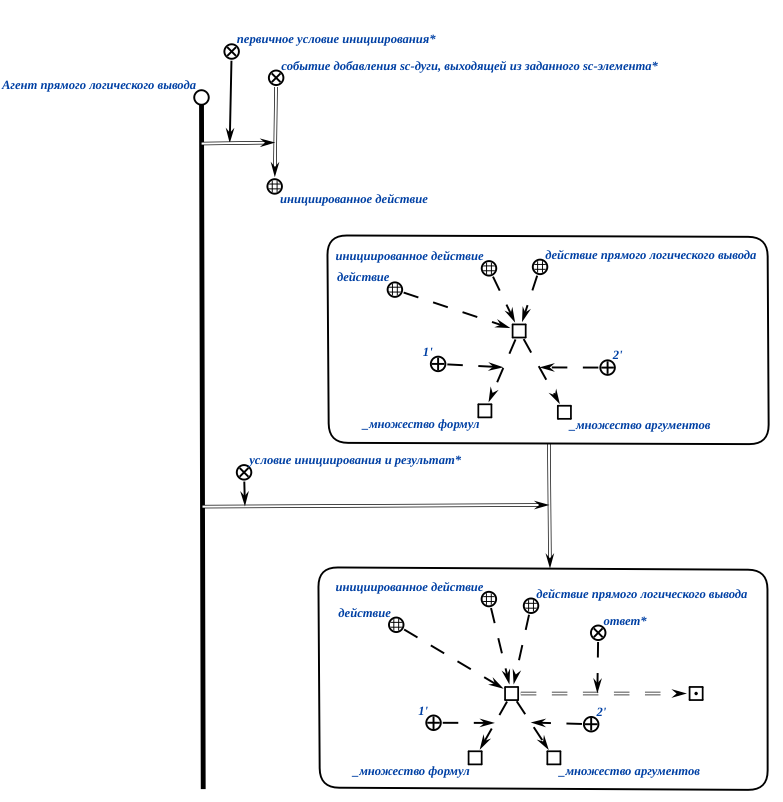
\includegraphics[scale=0.8]{author/part3/figures/direct_inference_agent.png}
	\caption{Спецификация агента прямого логического вывода}
	\label{fig:direct_inference_agent}
\end{figure}

\begin{figure}[H]
	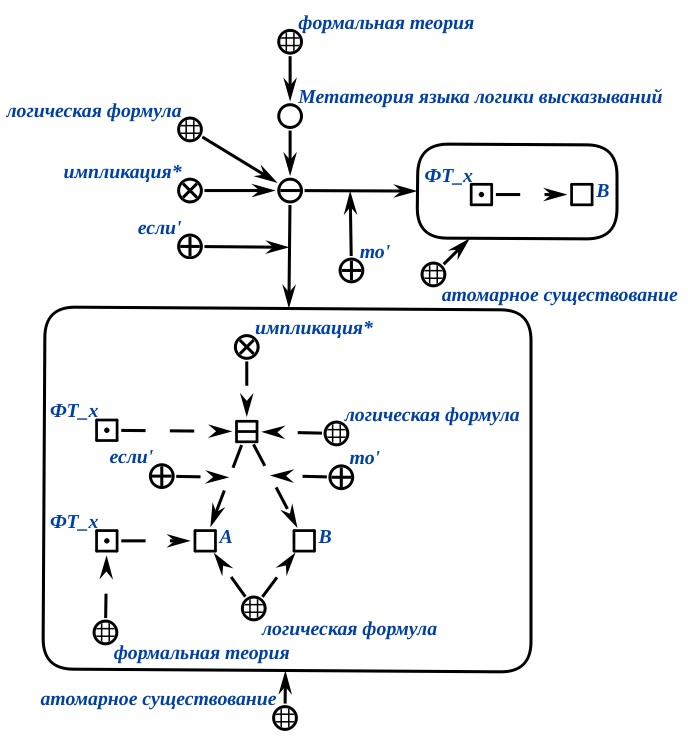
\includegraphics[scale=0.8]{author/part3/figures/Modus_ponens.png}
	\caption{Формализация правила вывода Modus ponens}
	\label{fig:modus_ponens}
\end{figure}

\begin{figure}[H]
	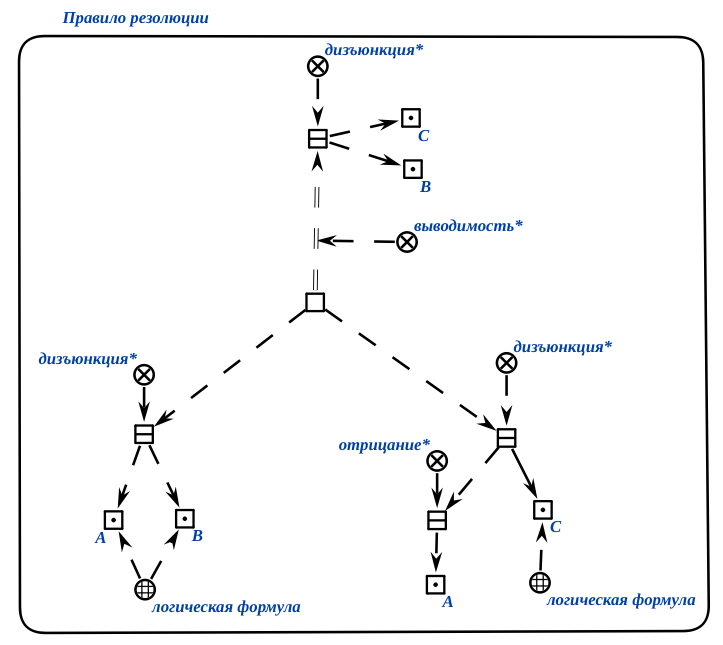
\includegraphics[scale=0.8]{author/part3/figures/resolution.png}
	\caption{Формализация правила резолюции}
	\label{fig:modus_ponens}
\end{figure}

\section{Языки продукционного программирования, используемые ostis-системами}
\subsection{Синтаксис языков продукционного программирования, используемых ostis-системами}
\subsection{Денотационная семантика языков продукционного программирования, используемых ostis-системами}
\subsection{Операционная семантика языков продукционного программирования, используемых ostis-системами}

%\input{author/references}
\chapter{Конвергенция и интеграция искусственных нейронных сетей с базами знаний в ostis-системах}
\chapauthortoc{Ковалев М.В.\\Крощенко А.А.\\Головко В.А.}
\label{chapter_ann}

\vspace{-7\baselineskip}

\begin{SCn}
	\begin{scnrelfromlist}{автор}
		\scnitem{Ковалев М.В.}
		\scnitem{Крощенко А.А.}
		\scnitem{Головко В.А.}
	\end{scnrelfromlist}

	\bigskip

	\scntext{аннотация}{В главе рассмотрен подход к \textit{интеграции} и \textit{конвергенции} \textit{искусственных нейронных сетей} с \textit{базами знаний} в \textit{интеллектуальных компьютерных системах нового поколения} с помощью представления и интерпретации \textit{искусственных нейронных сетей} в \textit{базе знаний}. Описаны \textit{Синтаксис, Денотационная и Операционная семантика Языка представления нейросетевых методов в базах знаний}. Описаны этапы построения \textit{нейросетевых методов решения задач} с помощью интеллектуальной среды проектирования \textit{искусственных нейронных сетей}.}

	\bigskip

	\begin{scnrelfromlist}{подраздел}
		\scnitem{\nameref{sec_chapter_ann_models}~\nameref{sec_chapter_ann_models}}
		\scnitem{\nameref{sec_chapter_ann_framework}~\nameref{sec_chapter_ann_framework}}
	\end{scnrelfromlist}

	\bigskip
	
	\begin{scnrelfromlist}{ключевой знак}
		\scnitem{Язык представления нейросетевых методов решения задач в базах знаний}
	\end{scnrelfromlist}

	\begin{scnrelfromlist}{ключевое понятие}
		\scnitem{нейросетевой метод решения задач}
		\scnitem{нейросетевая модель решения задач}
		\scnitem{навык решения задач с помощью искусственных нейронных сетей}
		\scnitem{действие по построению искусственных нейронных сетей}
	\end{scnrelfromlist}

	\bigskip

	\begin{scnrelfromlist}{библиографическая ссылка}
		\scnitem{\scncite{Standart2021}}
		\scnitem{\scncite{Castelvecchi2016}}
		\scnitem{\scncite{Ribeiro2016}}
		\scnitem{\scncite{Lundberg2017}}
		\scnitem{\scncite{Garcez2015}}
		\scnitem{\scncite{Besold2017}}
		\scnitem{\scncite{Golovko2019}}
		\scnitem{\scncite{Kroshchanka2022}}
		\scnitem{\scncite{Golovko2017}}
		\scnitem{\scncite{Kovalev2022}}
		\scnitem{\scncite{Glorot2010}}
		\scnitem{\scncite{He2015}}
		\scnitem{\scncite{Goodfellow2017}}
		\scnitem{\scncite{Haykin2006}}
		\scnitem{\scncite{Duchi2011}}
		\scnitem{\scncite{Kingma2014}}
	\end{scnrelfromlist}

\end{SCn}

\section*{Введение в Главу \ref{chapter_ann}}

Современные \textit{решатели задач} \textit{интеллектуальных систем} все чаще сталкиваются с необходимостью решения \textit{комплексных задач} с помощью различных традиционных и интеллектуальных \textit{методов решения задач} в едином информационном ресурсе (в пределе --- в единой \textit{базе знаний}).

С другой стороны, \textit{интеллектуальные компьютерные системы нового поколения} обладают, среди прочих, следующими способностями (см. \scncite{Standart2021}):
\begin{textitemize}
	\item способность постоянно повышать качество решения задач;
	\item способность приобретать навыки решения принципиально новых задач;
	\item способность обосновывать свои решения;
	\item способность находить и устранять ошибки в своих решения (способность к интроспекции).
\end{textitemize}

Представление различных \textit{методов решения задач} в единой \textit{базе знаний} обеспечивает \textit{семантическую совместимость} этих методов. Решая задачу с помощью таких методов, система не взаимодействует с ними по принципу \scnqq{входов-выходов}. Напротив, единая память позволяет отслеживать преобразование входных знаний в реальном времени с помощью любых имеющихся методов, что обеспечивает способность к интроспекции и способность объяснять решения системы.

Перспективными и активно развивающимися \textit{методами решения задач} являются \textbf{\textit{искусственные нейронные сети}} (и.н.с.), что обуславливается, с одной стороны, развитием теории \textit{и.н.с.}, а с другой --- аппаратных возможностей машин, которые используются для их обучения.

Достоинствами \textit{и.н.с.} можно назвать способность решения задач при неизвестных закономерностях, а так же способность решения задач без необходимости разработки проблемоориентированных подходов.

Большинство нейросетевых моделей работают как \scnqq{черный ящик} (см. \scncite{Castelvecchi2016}), что является одним из основных недостатков этого метода решения задач. Большой объем обрабатываемых этими моделями данных создает необходимость мониторинга, объяснения и понимания механизмов их работы с целью вербализации оценки и оптимизации деятельности \textit{и.н.с.}

Современные задачи все чаще требуют обоснования своего решения. Появилось целое направление \textit{Explainable AI}, в рамках которого предпринимаются различные попытки объяснить решения \textit{и.н.с.} (см. \scncite{Ribeiro2016}, \scncite{Lundberg2017}). Развиваются подходы, предлагающие интеграцию нейронных сетей с базами знаний (см. \scncite{Garcez2015}, \scncite{Besold2017}, \scncite{Golovko2019}, \scncite{Kroshchanka2022}).

Еще одним недостатком \textit{и.н.с.} можно назвать эвристический характер процесса подбора архитектур моделей и параметров их обучения и высокие требования к объему знаний проектировщиков нейросетевых моделей.

Исходя из перечисленных способностей, наличие которых необходимо обеспечивать в \textit{интеллектуальных компьютерных системах нового поколения}, встает проблема разработки подхода к интеграции \textit{и.н.с.} в \textit{базу знаний} \textit{интеллектуальной системы} как в качестве \textit{метода решения задач}, так и в качестве объекта автоматического проектирования новых методов. Решение этой проблемы позволит преодолеть указанные выше недостатки нейросетевого метода.

Можно выделить два основных направления \textit{интеграции и.н.с. с базами знаний} \:
\begin{textitemize}
	\item Построение \textit{интеллектуальных систем}, способных использовать \textit{нейросетевые методы решения задач} наравне с другими имеющимися в системе методами для решения \textit{комплексных задач}. Такие системы смогут учитывать семантику решаемых задач на более высоком уровне, что сделает решения более структурированными и прозрачными.
	\item Построение интеллектуальной среды по разработке, обучению и интеграции различных \textit{и.н.с.}, совместимых с \textit{базами знаний} через представление \textit{и.н.с.} с помощью онтологических структур и их интерпретацию средствами представления знаний. Такая среда предоставит возможность интроспекции \textit{и.н.с.}, возможность сохранения состояний \textit{и.н.с.} после обучения и реконфигурации сети, что позволит производить более глубокий анализ ее работы. Так же формальное описание знаний в рамках предметной области \textit{и.н.с.} поможет уменьшить порог вхождения разработчиков в область методов решения задач с помощью \textit{и.н.с.}
\end{textitemize}


\section{Модели искусственных нейронных сетей, используемых в ostis-системах}
\label{sec_chapter_ann_models}

\begin{SCn}
	\begin{scnrelfromlist}{подраздел}
		\scnitem{\nameref{subsec_ann_denot}~\nameref{subsec_ann_denot}}
		\scnitem{\nameref{subsec_ann_oper}~\nameref{subsec_ann_oper}}
	\end{scnrelfromlist}

	\bigskip

	\begin{scnrelfromlist}{ключевой знак}
		\scnitem{Язык представления нейросетевого метода решения задач в базах знаний}
		\scnitem{Денотационная семантика Языка представления нейросетевого метода решения задач в базах знаний}
		\scnitem{Операционная семантика Языка представления нейросетевого метода в базах знаний}
	\end{scnrelfromlist}

	\begin{scnrelfromlist}{ключевое понятие}
		\scnitem{нейросетевой метод решения задач}
		\scnitem{навык решения задач с помощью искусственных нейронных сетей}
		\scnitem{формальный нейрон}
		\scnitem{синаптическая связь}
		\scnitem{слой и.н.с.}
		\scnitem{взвешенной сумма нейрона}
	\end{scnrelfromlist}

	\begin{scnrelfromlist}{ключевое отношение}
		\scnitem{функция активации*}
		\scnitem{выходное значение\scnrolesign}
	\end{scnrelfromlist}
\end{SCn}

Как уже было описано в \textit{Главе \ref{chapter_actions} \nameref{chapter_actions}}, \textit{решатель задач} занимается обработкой фрагментов базы знаний. На операционном уровне обработка сводится к добавлению, поиску, редактированию и удалению sc-узлов и sc-коннекторов \textit{базы знаний}. На семантическом же уровне такая операция является \textit{действием, выполняемым в памяти субъекта действия}, где, в общем случае, субъектом является \textit{ostis-система}, а \textit{база знаний} --- ею памятью. \textit{действие} определяется как процесс воздействия одной сущности (или некоторого множества сущностей) на другую сущность (или на некоторое множество других сущностей) в соответствии с некоторой целью (см. \textit{Главу \ref{chapter_actions}~\nameref{chapter_actions}}).

Схожие задачи объединены в классы, для которых заданы обобщенные формулировки задач. Для \textit{и.н.с.} выделены следующие классы задач:
\begin{textitemize}
	\item \textit{задача классификации}. Задача построения классификатора, то есть отображения $\tilde c: X \rightarrow C$, где $ X \in \mathbb{R}^m$ --- признаковое пространство входного образа, $C = {C_1, C_2, ...C_k }$ --- конечное и обычно небольшое множество меток классов.
	\item \textit{задача регрессии}. Задача построения оценочной функции по примерам $(x_i, f(x_i))$, где $f(x)$ --- неизвестная функция. \textit{оценочная функция*} --- отображение вида $\tilde{f}: X \rightarrow \mathbb{R}$, где $X \in \mathbb{R}^m$ --- признаковое пространство входных данных.
	\item \textit{задача кластеризации}. Задача построения функции $a: X \rightarrow Y$, которая любому объекту $x \in X$ ставит в соответствие номер кластера $y \in Y$ в соответствие с определенной метрикой расстояния $\rho(x, x')$, где \textit{X} --- множество объектов, \textit{Y} --- множество номеров (имен, меток) кластеров, $x, x' \in X$.
	\item \textit{задача понижения размерности признакового пространства}. Задача построения функции $h: X \rightarrow Y$, сохраняющей заданные соотношения между точками множеств X и Y, где $X \subset \mathbb{R}^p$, $Y=h(X) \subset \mathbb{R}^q$, $q < p$.
	\item \textit{задача управления}. Задача построения модели-регулятора состояния сложного динамического объекта.
	\item \textit{задача фильтрации}. Задача построения модели, которая производит очистку исходного сигнала, содержащего некоторый шум и уменьшает влияние случайных ошибок в сигнале.
	\item \textit{задача детекции}. Является частным случаем задачи классификации и задачи регрессии. Задача построения модели, осуществляющей обнаружение объектов определенных типов на фото- и видеоизображениях.
	\item \textit{задача с ассоциативной памятью}. Задача построения модели, позволяющей выполнить реконструкцию исходного образа на основании сохраненных ранее образов.
\end{textitemize}

Для классов задач формулируются классы методов их решения. \textit{метод решения задач} определяется как \textit{программа}, которая может быть как процедурной, так и декларативной. В свою очередь, \textit{класс методов решения задач} определяется как множество всевозможных \textit{методов решения задач}, имеющих общий язык представления этих методов. \textit{язык представления методов} позволяет описывать \textit{синтаксическую}, \textit{денотационную} и \textit{операционную семантику} этого \textit{метода}.

Предлагается рассматривать \textit{и.н.с.} как класс методов решения задач со своим языком представления. Таким образом, искусственная нейронная сеть - это \textbf{\textit{нейросетевой метод решения задач}}. В соответствии с \textit{Технологией OSTIS}, спецификация класса методов решения задач сводится к спецификации соответствующего \textit{языка представления методов}, то есть к описанию его синтаксической, денотационной и операционной семантики.

Для достижения семантической совместимости с другими \textit{методами решения задач} \textit{Технологии OSTIS}, предлагается описывать нейросетевые методы внутри семантической памяти, соответственно, \textit{Синтаксис Языка представления \textit{нейросетевых методов решения задач в базах знаний}} является \textit{Синтаксисом SC-кода}, использующимся в \textit{Технологии OSTIS} для представления знаний.

Таким образом, чтобы добавить в арсенал \textit{Технологии OSTIS} \textit{нейросетевые методы решения задач} и тем самым расширить круг задач, решаемых ostis-системами, необходимо описать денотационную и операционную семантику \textbf{\textit{Языка представления нейросетевого метода решения задач в базах знаний}}.

\textbf{\textit{Денотационная семантика Языка представления нейросетевого метода решения задач в базах знаний}} описывается в рамках предметной области и соответствующей ей онтологии нейросетевого метода.

Операционной семантикой любого \textit{языка представления методов решения задач} является спецификация семейства агентов, обеспечивающих интерпретацию любого метода, принадлежащего соответствующему классу методов. Это семейство является интерпретатором соответствующего метода решения задач. В рамках технологии OSTIS такой интерпретатор называется \textit{моделью решения задач}. Так как в рамках \textit{Технологии OSTIS} используется многоагентный подход, то разработка нейросетевой модели решения задач сводится к разработке агентно-ориентированной модели интерпретации \textit{и.н.с.}

Понятие \textit{навыка} описывает метод, интерпретация которого полностью может быть осуществлена данной кибернетической системой, в памяти которой хранится указанный метод. Таким образом, формируя спецификацию в ostis-системе для нейросетевого метода решения задач и нейросетевой модели решения задач можно говорить о наличии у такой системы \textbf{\textit{навыка решения задач с помощью и.н.с.}}.

На рисунке \textit{\nameref{fig:actions_concepts}} представлен фрагмент теоретико-множественной онтологии \textit{и.н.с.}, описывающий связь таких понятий и узлов, как:
\begin{textitemize}
	\item класс задач, решаемых с помощью и.н.с.(для примера, взят класс задач классификации);
	\item класс нейросетевых методов решения задач;
	\item нейросетевая модель решения задач;
	\item навык решения задач с помощью и.н.с.;
	\item конкретные задачи и методы их решения (для примера взята конкретная обученная сверточная и.н.с.).
\end{textitemize}

\begin{figure}[H]
	\caption{SCg-текст. Фрагмент теоретико-множественной онтологии и.н.с.}
	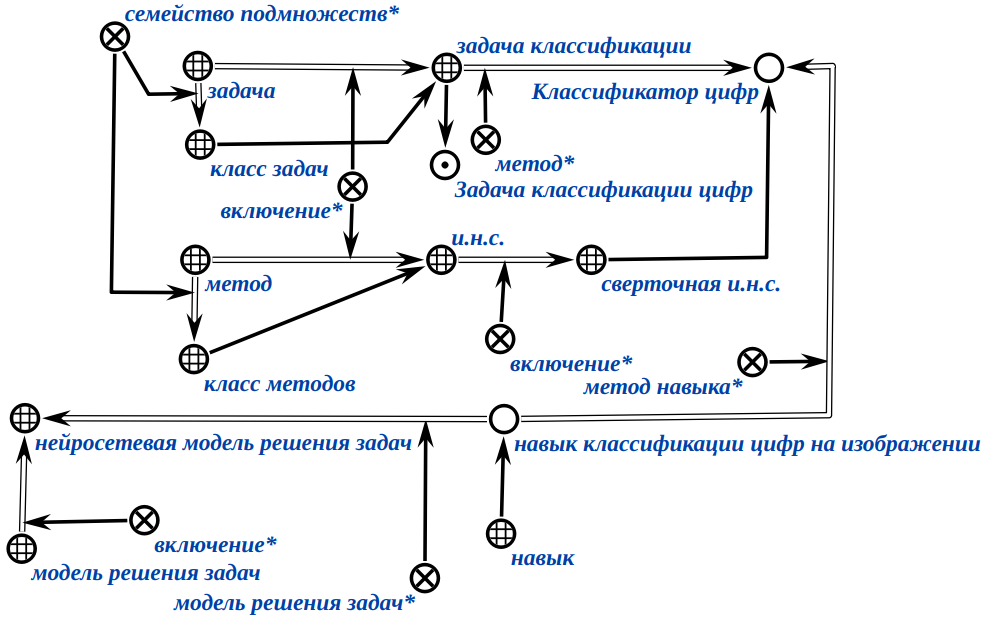
\includegraphics[scale=0.5]{author/part3/figures/actions_concepts.png}
	\label{fig:actions_concepts}
\end{figure}

Использование \textit{и.н.с.} как\textit{ метода решения задач} подразумевает использование уже спроектированной и обученной \textit{и.н.с.} Однако наличие языка описания нейросетевого метода решения задач в памяти \textit{ostis-системы} открывает дорогу для автоматизации самих процессов проектирования и обучения \textit{и.н.с.} Такая автоматизация представляется отдельными классами задач и соответствующими навыками их решения. Подход к такой автоматизации описан в \textit{\ref{sec_chapter_ann_framework} \nameref{sec_chapter_ann_framework}}.

\subsection{Денотационная семантика моделей искусственных нейронных сетей, используемых в ostis-системах}
\label{subsec_ann_denot}

Как уже было сказано, \textit{Денотационная семантика Языка представления нейросетевых методов в базах знаний} описывается в рамках предметной области и соответствующей ей онтологии нейросетевого метода

Максимальным классом объектов исследования предметной области искусственных нейронных сетей является \textit{искусственная нейронная сеть}.

\begin{SCn}
	\scnheader{искусственная нейронная сеть}
	\scnidtf{и.н.с.}
	\scnidtf{нейросетевой метод }
	\scnidtf{множество искусственных нейронных сетей}
	\scnidtf{нейронная сеть}
	\scntext{пояснение}{Cовокупность нейронных элементов и связей между ними (см. \scncite{Golovko2017}).}
\end{SCn}

Искусственная нейронная сеть состоит из \textbf{\textit{формальных нейронов}}, которые связаны между собой посредством \textbf{\textit{синаптических связей}}. Нейроны организованы в \textbf{\textit{слои}}. Каждый нейрон слоя принимает сигналы со входящих в него синаптических связей, обрабатывает их единым образом с помощью заданной ему или всему слою \textbf{\textit{функции активации}} и передает результат на выходящие из него синаптические связи.

Архитектурой \textit{и.н.с.} будем называть совокупность информации о структуре ее слоев, формальных нейронов, синаптических связей и функций активаций. То есть то, что можно обучить и использовать для решения задач.

Пример архитектуры \textit{и.н.с.} представлен на рисунке \textit{\nameref{fig:nn_example}}.

\begin{figure}[H]
	\caption{Рисунок. Пример архитектуры и.н.с.}
	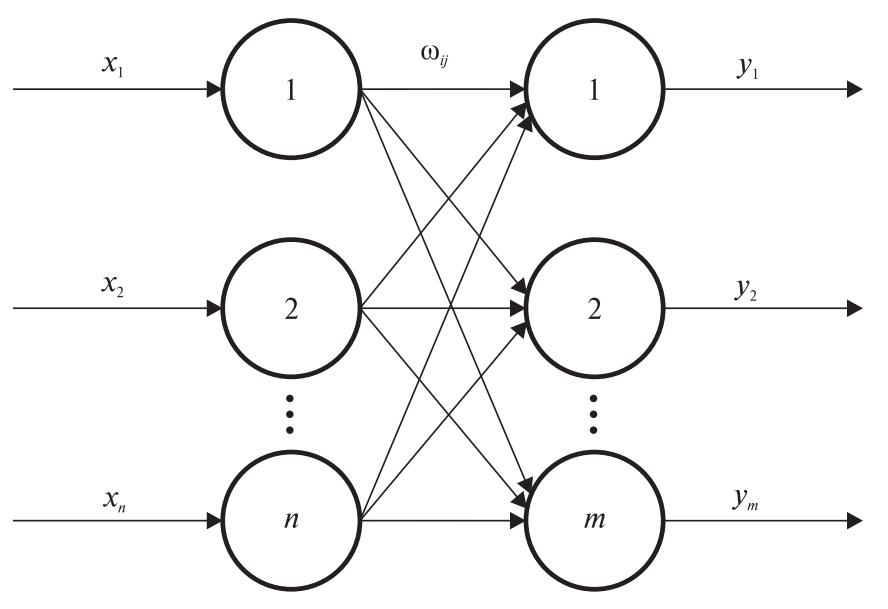
\includegraphics[scale=0.3]{author/part3/figures/neural_network.png}
	\label{fig:nn_example}
\end{figure}

В соответствии с тем, какая у \textit{и.н.с.} архитектура, можно выделить следующую иерархию классов \textit{и.н.с.} Рассмотрим эту иерархию в \textit{SCn-коде}.

\begin{SCn}
	\scnheader{искусственная нейронная сеть}
	\scnidtf{нейросетевой метод}
	\scnrelto{включение}{метод}
	\scnrelfrom{разбиение}{Типология и.н.с. по признаку направленности связей\scnsupergroupsign}
	\begin{scnindent}
		\begin{scneqtoset}
			\scnitem{и.н.с. с прямыми связями}
			\begin{scnrelfromset}{декомпозиция}
				\scnitem{персептрон}
				\begin{scnrelfromset}{декомпозиция}
					\scnitem{персептрон Розенблатта}
					\scnitem{автоэнкодерная и.н.с.}
				\end{scnrelfromset}
				\scnitem{машина опорных векторов}
				\scnitem{и.н.с. сеть радиально-базисных функций}
				\scnitem{сверточная и.н.с.}
			\end{scnrelfromset}
			\scnitem{и.н.с. с обратными связями}
			\begin{scnrelfromset}{декомпозиция}
				\scnitem{и.н.с. Хопфилда}
				\scnitem{и.н.с. Хэмминга}
			\end{scnrelfromset}
			\scnitem{рекуррентная искусственная нейронная сеть}
			\begin{scnrelfromset}{декомпозиция}
				\scnitem{и.н.с. Джордана}
				\scnitem{и.н.с. Элмана}
				\scnitem{мультирекуррентная и.н.с.}
				\scnitem{LSTM-элемент}
				\scnitem{GRU-элемент}
			\end{scnrelfromset}
		\end{scneqtoset}
	\end{scnindent}
	\scnrelfrom{разбиение}{Типология и.н.с. по признаку полноты связей\scnsupergroupsign}
	\begin{scnindent}
		\begin{scneqtoset}
			\scnitem{полносвязная и.н.с.}
			\scnitem{слабосвязная и.н.с.}
		\end{scneqtoset}
	\end{scnindent}
\end{SCn}

Рассмотрим архитектурные компоненты подробнее.
\begin{SCn}
	\scnheader{формальный нейрон}
	\scnidtf{искусственный нейрон}
	\scnidtf{нейрон}
	\scnidtf{ф.н.}
	\scnidtf{нейронный элемент}
	\scnidtf{множество нейронов искусственных нейронных сетей}
	\scnidtf{математическая модель биологического нейрона}
	\scnsubset{искусственная нейронная сеть}
	\scntext{пояснение}{Основной элемент \textit{и.н.с.}, применяющий свою \textit{функцию активации} (см. \scncite{Golovko2017}) к сумме произведений входных сигналов на весовые коэффициенты:
		\begin{equation*}
			y = F\left(\sum_{i=1}^{n} w_ix_i - T\right) = F(WX - T)
		\end{equation*}
		где $X = (x_1,x_2,...,x_n)^{T}$ --- вектор входного сигнала; $W - (w_1,w_2,...,w_n)$ --- вектор весовых коэффициентов; \textit{T} --- пороговое значение;
		\textit{F} --- \textit{функция активации}.}
\end{SCn}

Отдельный \textit{формальный нейрон} является \textit{искусственной нейронной сетью} с одним нейроном в единственном слое.
\textit{формальные нейроны} могут быть классифицированы следующим образом:
\begin{textitemize}
	\item Полносвязный \textit{формальный нейрон} --- нейрон, у которого есть полный набор связей с нейронами предшествующего слоя. Oтдельный обрабатывающий элемент \textit{и.н.с.}, выполняющий функциональное преобразование взвешенной суммы элементов вектора входных значений с помощью \textit{функции активации}.
	\item Сверточный \textit{формальный нейрон} --- отдельный обрабатывающий элемент \textit{и.н.с.}, выполняющий функциональное преобразование результата операции свертки матрицы входных значений с помощью \textit{функции активации}. Сверточный \textit{формальный нейрон} может быть представлен полносвязным \textit{формальным нейроном}.
	\item Рекуррентный \textit{формальный нейрон} --- нейрон, имеющий обратную связь с самим собой или с другими нейронами \textit{и.н.с.}.
\end{textitemize}

Схематически \textit{формальный нейрон} можно представить в виде следующей модели (рисунок \textit{\nameref{fig:formal_neuron}}).

\begin{figure}[H]
	\caption{SCg-текст. Формальный нейрон}
	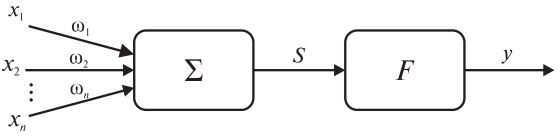
\includegraphics[scale=0.4]{author/part3/figures/formal_neuron.png}
	\label{fig:formal_neuron}
\end{figure}

Определим понятия \textit{синаптической связи} и \textit{слоя и.н.с.}:

\begin{SCn}
	\scnheader{синаптическая связь}
	\scnidtf{синапс}
	\scnsubset{ориентированная пара}
	\scntext{пояснение}{ориентированная пара, первым компонентом которой является нейрон, из
	которого исходит сигнал, а вторым компонентом --- нейрон, который принимает этот сигнал}

	\scnheader{слой и.н.с.}
	\scnidtf{слой}
	\scnidtf{слой искусственной нейронной сети}
	\scnidtf{множество слоев искусственных нейронных сетей}
	\scnsubset{искусственная нейронная сеть}
	\scntext{пояснение}{множество нейронных элементов, на которые в каждый такт времени
	параллельно поступает информация от других нейронных элементов сети (см. \scncite{Golovko2017})}
	\scntext{пояснение}{множество формальных нейронов, осуществляющих параллельную независимую обработку вектора или матрицы входных значений}
\end{SCn}

Отдельный слой является искусственной нейронной сетью с одним слоем.
Следует отметить принципиальную важность этого замечания. Один \textit{слой и.н.с.} уже является нейронной сетью, поскольку над ним можно производить все основные операции, которые производятся над \scnqq{большой} \textit{и.н.с.} (его можно обучить и использовать для решения определенной задачи).

\textit{слои и.н.с.} могут быть классифицированы следующим образом (по признаку операции, осуществляемой слоем):
\begin{textitemize}
	\item \textit{полносвязный слой и.н.с.} --- слой, в котором каждый нейрон является полносвязным;
	\item \textit{сверточный слой и.н.с.} --- слой, в котором каждый нейрон является сверточным;
	\item \textit{слой и.н.с.} нелинейного преобразования --- слой, осуществляющий нелинейное преобразование входных данных;
	\item \textit{dropout слой и.н.с.} --- слой, реализующий технику регуляризации dropout;
	\item \textit{pooling слой и.н.с.} --- подвыборочный слой;
	\item \textit{слой и.н.с.} батч-нормализации.
\end{textitemize}

Как правило, слой нелинейного преобразования выделяется в отдельный слой только в программных реализациях. Фактически он рассматривается как финальный этап расчета выходной активности любого нейрона --- применение \textit{функции активации}.

\textit{dropout-слой} функционирует только во время обучения \textit{и.н.с.}. Поскольку полносвязные слои имеют большое количество настраиваемых параметров, они подвержены эффекту \textit{переобучения}. Один из способов устранить такой негативный эффект --- выполнить частичный отсев результатов на выходе полносвязного слоя. На этапе обучения техника dropout позволяет отбросить выходную активность некоторых нейронов с определенной, заданной вероятностью. Выходная активность \scnqq{отброшенных} нейронов полагается равной нулю.

Назначение подвыборочного слоя --- в осуществлении уменьшения размерности входных данных.

Нужно отметить, что данный перечень неполный --- разновидности \textit{слоев и.н.с.} появляются практически в каждой заслуживающей внимания публикации по нейросетевым алгоритмам и на текущий момент их существует достаточно много, однако, как правило, при построении более традиционных архитектур ограничиваются только приведенными вариантами слоев.

\textit{слои и.н.с.} также могут быть классифицированы по исполняемой роли в рамках архитектуры (место в последовательности \textit{слоев и.н.с.}).

Так, например, слой, расположенный первым, называется распределяющим. Слои, расположенные далее, за исключением последнего, называются обрабатывающими. Наконец, последний слой носит название выходного \textit{слоя и.н.с.}

Последний архитектурный компонент \textit{и.н.с.} --- это функция активации:

\begin{SCn}
	\scnheader{функция активации*}
	\scnidtf{функция активации нейрона*}
	\scniselement{неролевое отношение}
	\scniselement{бинарное отношение}
	\scntext{пояснение}{неролевое отношение, связывающее \textit{формальный нейрон} с функцией, результат
	применения которой к \textbf{\textit{взвешенной сумме нейрона}} определяет его \textbf{\textit{выходное значение}}.}
	\scnrelfrom{первый домен}{формальный нейрон}
	\scnrelfrom{второй домен}{функция}
\end{SCn}

Перечислим некоторые, наиболее известные и применяемые типы функций активации:
\begin{textitemize}
	\item линейная функция\\
	\scntext{формула}{
		\begin{equation*}
			y = kS
		\end{equation*}
		где \textit{k} --- коэффициент наклона прямой, \textit{S} --- в.с.;
	}
	\item пороговая функция\\
	\scntext{формула}{
		\begin{equation*}
			y = sign(S) =
			\begin{cases}
				1, S > 0,\\
				0, S \leq 0
			\end{cases}
		\end{equation*};
	}
	\item сигмоидная функция\\
	\scntext{формула}{
		\begin{equation*}
			y = \frac{1}{1+e^{-cS}}
		\end{equation*}
		где \textit{с} > 0 --- коэффициент, характеризующий ширину сигмоидной функции по оси абсцисс, \textit{S} --- в.с.;
	}
	\item функция гиперболического тангенса\\
	\scntext{формула}{
		\begin{equation*}
			y = \frac{e^{cS}-e^{-cS}}{e^{cs}+e^{-cS}}
		\end{equation*}
		где \textit{с} > 0 --- коэффициент, характеризующий ширину сигмоидной функции по оси абсцисс, \textit{S} --- в.с.;
	}
	\item функция softmax\\
	\scntext{формула}{
		\begin{equation*}
			y_j = softmax(S_j) = \frac{e^{S_j}}{\sum_{j} e^{S_j}}
		\end{equation*}
		где $S_j$ --- в.с. \textit{j}-го выходного нейрона;
	}
	\item функция ReLU\\
	\scntext{формула}{
		\begin{equation*}
			y = F(S) =
			\begin{cases}
				S, S > 0,\\
				kS, S \leq 0
			\end{cases}
		\end{equation*}
		где \textit{k} = 0 или принимает небольшое значение, например, 0.01 или 0.001.
	}
\end{textitemize}

В рамках \textit{предметной области} формализована иерархия параметров \textit{и.н.с.}
\begin{SCn}
	\scnheader{параметр и.н.с.}
	\scnsubset{параметр}
	\scnrelfrom{разбиение}{}
	\begin{scnindent}
		\begin{scneqtoset}
			\scnitem{настраиваемый параметр и.н.с.}
			\begin{scnrelfromset}{декомпозиция}
				\scnitem{весовой коэффициент синаптической связи}
				\scnitem{пороговое значение}
				\scnitem{ядро свертки}
			\end{scnrelfromset}
			\scnitem{архитектурный параметр и.н.с.}
			\begin{scnrelfromset}{декомпозиция}
				\scnitem{количество слоев}
				\scnitem{количество нейронов}
				\scnitem{количество синаптических связей}
			\end{scnrelfromset}
		\end{scneqtoset}
	\end{scnindent}
\end{SCn}

Так же в \textit{Предметную область нейросетевых методов} добавлены понятия для описания метрик эффективности \textit{нейросетевых методов}. Данные метрики учитываются \textit{решателем задач} при принятии решения об использовании того или иного \textit{нейросетевого метода}.

Метрики могут быть классифицированы по типу решаемой задачи.
\begin{SCn}
	\scnheader{метрика оценки качества и.н.с.}
	\scnrelfrom{разбиение}{Типология метрик по признаку решаемой задачи\scnsupergroupsign}
	\begin{scnindent}
		\begin{scneqtoset}
			\scnitem{классификационные метрики}
			\begin{scnrelfromset}{декомпозиция}
				\scnitem{точность и.н.с.}
				\scnitem{полнота и.н.с.}
				\scnitem{F1-метрика}
			\end{scnrelfromset}
			\scnitem{регрессионные метрики}
			\begin{scnrelfromset}{декомпозиция}
				\scnitem{MAE}
				\scnitem{MAPE}
				\scnitem{RMSE}
			\end{scnrelfromset}
		\end{scneqtoset}
	\end{scnindent}

	\scnheader{точность и.н.с.}
	\scnidtf{precision}
	\scnidtf{доля верно идентифицированных положительных исходов в общем числе исходов, которые были идентифицированы как положительные}
	\scntext{формула}{
		\begin{equation*}
			PRE = \frac{TP}{TP + FP}
		\end{equation*}
		где \textit{TP} и \textit{FP} --- число истинно-положительных и ложно-положительных предсказаний нейронной сети соответственно
	}

	\scnheader{полнота и.н.с.}
	\scnidtf{recall}
	\scnidtf{доля верно идентифицированных положительных исходов в общем числе положительных исходов}
	\scntext{формула}{
		\begin{equation*}
			REC = \frac{TP}{TP + FN}
		\end{equation*}
		где \textit{TP} и \textit{FN} --- число истинно-положительных и ложно-отрицательных предсказаний нейронной сети соответственно
	}

	\scnheader{F1-метрика}
	\scntext{формула}{
		\begin{equation*}
			F1 = 2 * \frac{PRE * REC}{PRE + REC}
		\end{equation*}
		где \textit{PRE} и \textit{REC} --- точность и полнота и.и.с. соответственно
	}

	\scnheader{MAE}
	\scnidtf{mean absolute error}
	\scntext{формула}{$\frac{1}{N} \sum_{i=1}^N |y_{etalon}^i - y_{predicted}^i|$,\\ $y_{etalon}^i$ --- эталонное значение,\\ $y_{predicted}^i$ --- значение, полученное и.н.с.,\\ \textit{N} --- объем обучающей выборки
	}
\end{SCn}

\begin{SCn}
	\scnheader{MAPE}
	\scnidtf{mean absolute percentage error}
	\scntext{формула}{$\frac{1}{N} \sum_{i=1}^N \frac{|y_{etalon}^i - y_{predicted}^i|}{y_{etalon}^i} * 100\%$, \\ $y_{etalon}^i$ --- эталонное значение,\\ $y_{predicted}^i$ --- значение, полученное и.н.с.,\\ \textit{N} --- объем обучающей выборки
	}
\end{SCn}

\begin{SCn}
	\scnheader{RMSE}
	\scnidtf{root mean squared error}
	\scntext{формула}{$\sqrt{\frac{1}{N} \sum_{i=1}^N (y_{etalon}^i - y_{predicted}^i)^2}$, \\ $y_{etalon}^i$ --- эталонное значение,\\ $y_{predicted}^i$ --- значение, полученное и.н.с.,\\ \textit{N} --- объем обучающей выборки
	}
\end{SCn}

С помощью выделенных понятий становится возможна формализация в \textit{базе знаний} архитектуры конкретных \textit{и.н.с.} В качестве примера, на рисунке \textit{\nameref{fig:neural_network_scg}} представлен пример формализации полносвязной двухслойной \textit{и.н.с.} с двумя нейронами на входном слое и одном нейроне на обрабатывающем слоев.

\begin{figure}
	\caption{SCg-текст. Пример формализации архитектуры искусственной нейронной сети в базе знаний}
	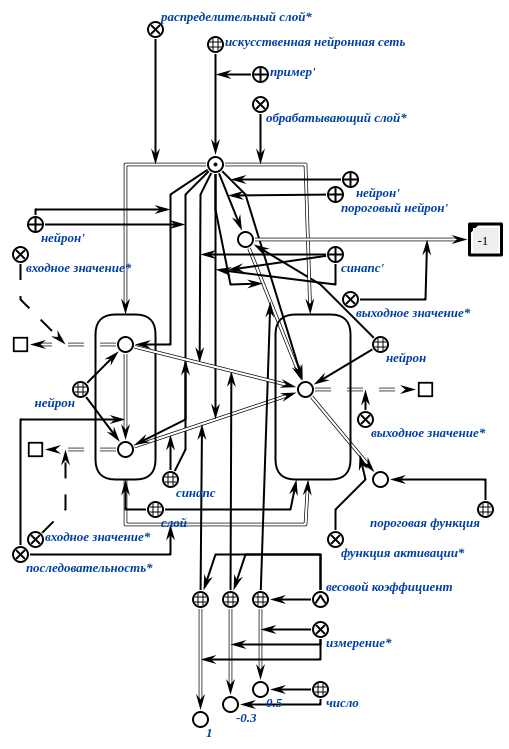
\includegraphics[width=0.8\linewidth]{author/part3/figures/neural_network_scg.png}
	\label{fig:neural_network_scg}
\end{figure}

Следует отметить, что в практике авторов еще не было необходимости явно представлять и.н.с., как это показано на рисунке \textit{\nameref{fig:neural_network_scg}}. Чаще всего, представление и.н.с. сводилось к представлению ее операционной семантики в виде SCP-программы, как это будет показано далее.

\subsection{Операционная семантика моделей искусственных нейронных сетей, используемых в ostis-системах}
\label{subsec_ann_oper}

\textbf{\textit{Операционная семантика Языка представления нейросетевого метода в базах знаний}} задается \textit{многоагентный подход} к интерпретации \textit{искусственных нейронных сетей} и спецификацией соответствующих действий.

Нейросетевой метод описан в виде программы на некотором \textit{языке программирования}, который может быть как внешним по отношению к \textit{ostis-системе}, так и внутренним (на данный момент, \textit{Язык SCP}). Каждому такому \textit{языку программирования} соответствует некоторая дочерняя \textit{предметная область} \textit{Предметная область нейросетевых методов} (см. \scncite{Kovalev2022}).

\begin{SCn}
	\scnheader{Предметная область нейросетевых методов}
	\scnidtf{Предметная область искусственных нейронных сетей}
	\begin{scnrelfromset}{дочерняя предметная область}
		\scnitem{Предметная область нейросетевых методов SCP}
		\scnitem{Предметная область нейросетевых методов Python}
		\scnitem{Предметная область нейросетевых методов C++}
	\end{scnrelfromset}
\end{SCn}

В случае описания \textit{нейросетевого метода} на внешнем языке, такой метод описывается в соответствующей предметной области, в рамках которой также специфицируется действие интерпретации данного метода. Данному действию соответствует агент, реализованный на соответствующем \textit{языке программирования}.

Однако для достижения конвергенции и интеграции необходимо описывать нейросетевые методы на внутреннем языке ostis-системы, которым является \textit{Язык SCP}.
Интерпретация \textit{scp-программы} сводится к агентно-ориентированной обработке действий в sc-памяти. Этими действиями являются \textit{scp-операторы}.

\begin{SCn}
	\scnheader{действие интерпретации слоя и.н.с.}
	\begin{scnrelfromset}{декомпозиция}
		\scnitem{действие вычисления взвешенной суммы всех нейронов слоя}
		\scnitem{действие вычисления функции активации всех нейронов слоя}
		\scnitem{действие интерпретации сверточного слоя}
		\scnitem{действие интерпретации пулинг слоя}
	\end{scnrelfromset}
\end{SCn}

Для описания спецификации указанных действий необходимо ввести понятия \textit{ориентированного множества чисел} и \textit{матрицы}, с помощью которых задаются входные значения \textit{и.н.с.}, выходные значения \textit{и.н.с.}, матрицы весовых коэффициентов и прочее.

Каждый элемент ориентированного множества чисел является некоторым числом. Числа могут быть представлены в виде sc-узлов, либо с помощью строкового представления всего множества, для чего используется специальное отношение \textit{строковое представление ормножества чисел*}, которое введено в целях оптимизации некоторых вариантов реализации агента, интерпретирующего действие, использующее понятие ориентированного множества чисел.

\begin{SCn}
	\scnheader{ориентированное множество чисел}
	\scnidtf{ормножество чисел}
	\scnrelto{включение}{число}
	\scnrelto{включение}{ориентированное множество}
	\scnrelto{первый домен}{строковое представление ормножества чисел*}
\end{SCn}

\textit{матрица} является \textit{ориентированным множеством} \textit{ориентированных множеств} чисел равной мощности.


\textbf{1. Действие вычисления взвешенной суммы всех нейронов слоя}

Аргументы(\textit{объекты'}) этого действия задаются следующими отношениями:
\begin{SCn}
	\scnheader{входной вектор'}
	\scnrelfrom{первый домен}{действие интерпретации и.н.с.}
	\scnrelfrom{второй домен}{ориентированное множество чисел}
\end{SCn}

\begin{SCn}
	\scnheader{матрица весовых коэффициентов нейронов слоя'}
	\scnrelfrom{первый домен}{действие по обработке и.н.с.}
	\scnrelfrom{второй домен}{матрица}
\end{SCn}

Результатом действия(\textit{результат'}) является ориентированное множество чисел, являющихся взвешенной суммой нейронов соответствующего слоя.

Пример спецификации действия вычисления взвешенной суммы всех нейронов слоя для слоя с двумя нейронами и входным вектором размерностью 2 приведен на рисунке \textit{\nameref{fig:action_weighted_sum}}.

\begin{figure}
	\caption{SCg-текст. Пример действия вычисления взвешенной суммы всех нейронов слоя}
	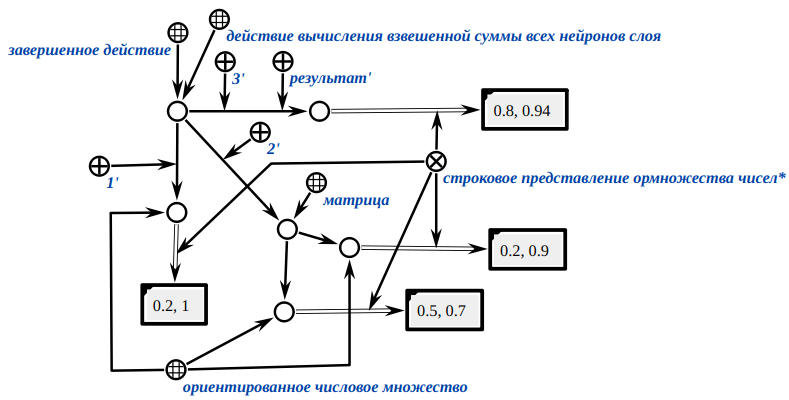
\includegraphics[width=0.95\linewidth]{author/part3/figures/action_weighted_sum.png}
	\label{fig:action_weighted_sum}
\end{figure}


\textbf{2. Действие вычисления функции активации всех нейронов слоя}

Аргументы этого действия задаются следующими отношениями:
\begin{SCn}
	\scnheader{вектор взвешенных сумм нейронов слоя'}
	\scnrelfrom{первый домен}{действие по обработке и.н.с.}
	\scnrelfrom{второй домен}{ориентированное множество чисел}

	\scnheader{вектор порогов нейронов слоя'}
	\scnrelfrom{первый домен}{действие по обработке и.н.с.}
	\scnrelfrom{второй домен}{ориентированное множество чисел}

	\scnheader{функция активации'}
	\scnrelfrom{первый домен}{действие по обработке и.н.с.}
	\scnrelfrom{второй домен}{функция}
\end{SCn}

Результатом действия является ориентированное множество чисел, являющихся выходными значениями нейронов слоя.


\textbf{3. Действие интерпретации сверточного слоя}

Аргументы этого действия задаются следующими отношениями:
\begin{SCn}
	\scnheader{входная матрица'}
	\scnrelfrom{первый домен}{действие интерпретации и.н.с.}
	\scnrelfrom{второй домен}{матрица}

	\scnheader{ядро свертки'}
	\scnrelfrom{первый домен}{действие интерпретации сверточного слоя}
	\scnrelfrom{второй домен}{матрица}

	\scnheader{шаг свертки'}
	\scnrelfrom{первый домен}{действие интерпретации сверточного слоя}
	\scnrelfrom{второй домен}{число}
\end{SCn}

Результатом действия является матрица, полученная в результате свертки входной матрицы с ядром свертки.


\textbf{4. Действие интерпретации пулинг слоя}

Аргументы этого действия задаются следующими отношениями:
\begin{SCn}
	\scnheader{входная матрица'}
	\scnrelfrom{первый домен}{действие интерпретации и.н.с.}
	\scnrelfrom{второй домен}{матрица}

	\scnheader{размер окна пулинга'}
	\scnrelfrom{первый домен}{действие интерпретации пулинг слоя}
	\scnrelfrom{второй домен}{матрица}

	\scnheader{размер окна пулинга'}
	\scnrelfrom{первый домен}{действие интерпретации пулинг слоя}
	\scnrelfrom{второй домен}{матрица}

	\scnheader{шаг окна пулинга'}
	\scnrelfrom{первый домен}{действие интерпретации пулинг слоя}
	\scnrelfrom{второй домен}{число}
\end{SCn}

Результатом действия является матрица, полученная в результате пулинга входной матрицы.

При необходимости задавать различные аргументы для нейронов одного и того же слоя, можно специфицировать соответствующие действия, однако на данный момент этого не было произведено из-за слабой изученности подобного рода \textit{нейросетевых моделей решения задач}.

Спецификация агентов, соответствующих указанным действиям, задает агентно-ориентированную модель интерпретации искусственных нейронных сетей. Реализация этой модели будет называться интерпретатором искусственных нейронных сетей

Рассмотрим пример описания на \textit{нейросетевого метода}, решающего задачу, которая формулируется следующим образом: вычислить результат логической операции ``ИСКЛЮЧАЮЩЕЕ ИЛИ'' для значений двух логических переменных. На рисунке \textit{\nameref{fig:strong_or_graphic}} представлено решение этой задачи с помощью сигнальной функции.

\begin{figure}
	\caption{Рисунок. Решение задачи \scnqq{ИСКЛЮЧАЮЩЕЕ ИЛИ}}
	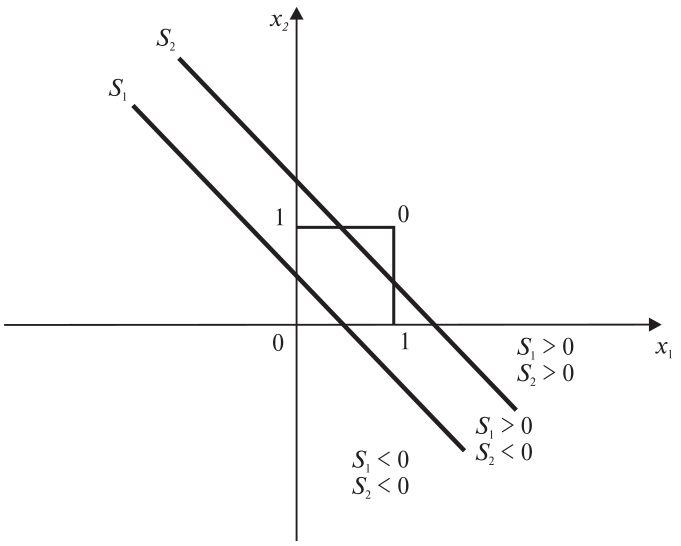
\includegraphics[width=0.5\linewidth]{author/part3/figures/strong_or_graphic.png}
	\label{fig:strong_or_graphic}
\end{figure}

В работе \scncite{Golovko2017} описан однослойный персептрон, решающий поставленную задачу. Персептрон состоит из двух входных нейронов и одного выходного, с заданным порогом в 0,5 и сигнальной функцией активации:
\begin{equation*}
	F(S) =
	\begin{cases}
		1, 0 < S < 0,\\
		0, else
	\end{cases}
\end{equation*}

Весовые коэффициенты синапсов входного слоя равны 1. На рисунке \textit{\nameref{fig:strong_or_ann}} представлена схема персептрона.

\begin{figure}
	\caption{Рисунок. Схема однослойного персептрона, решающего задачу \scnqq{ИСКЛЮЧАЮЩЕЕ ИЛИ}}
	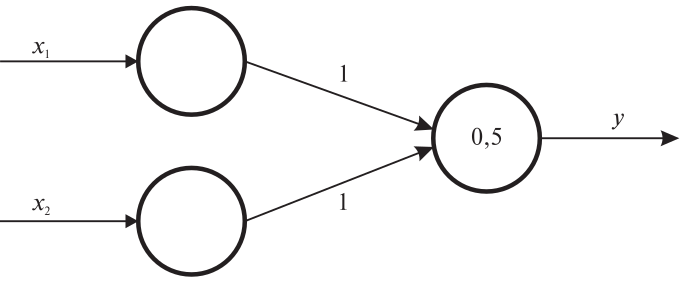
\includegraphics[width=0.5\linewidth]{author/part3/figures/strong_or_ann.png}
	\label{fig:strong_or_ann}
\end{figure}

Данному персептрону соответствует метод, представленный в базе знаний ostis-системы на описанном в этой главе языке представления нейросетевых методов SCP. Данный метод представлен на рисунке \textit{\nameref{fig:exclusive_or_ann_scp}}.

\begin{figure}
	\caption{Рисунок. Метод, решающий задачу \scnqq{ИСКЛЮЧАЮЩЕЕ ИЛИ}, представленный с помощью языка представления нейросетевых методов SCP}
	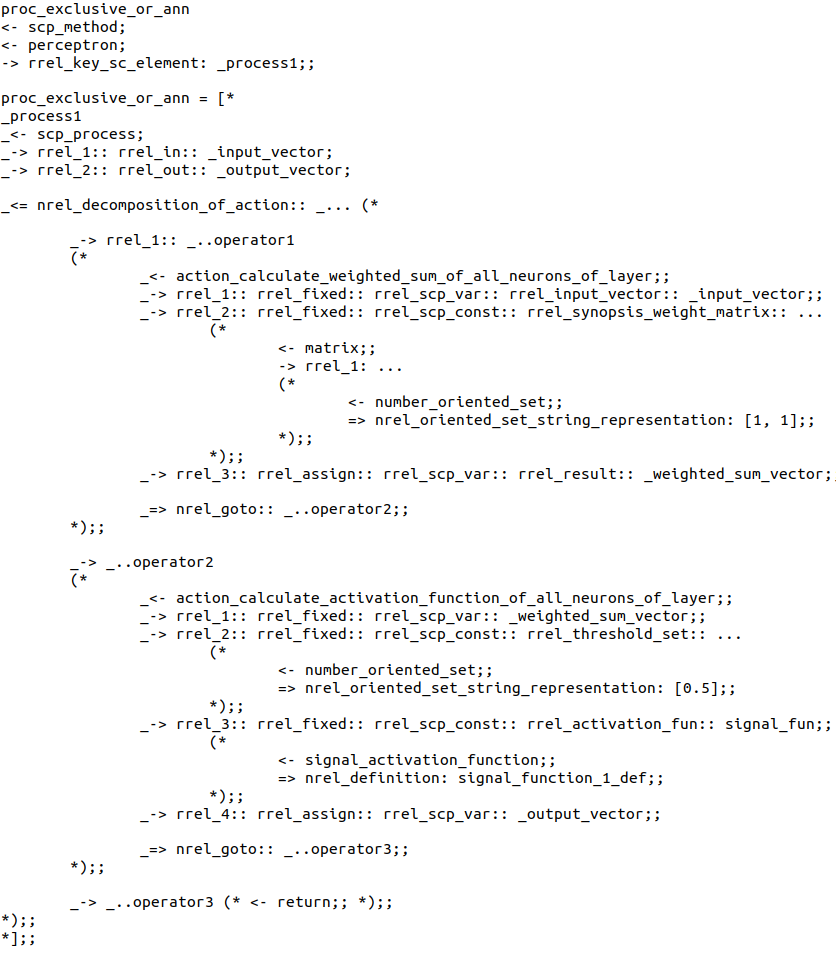
\includegraphics[width=0.95\linewidth]{author/part3/figures/exclusive_or_ann_scp.png}
	\label{fig:exclusive_or_ann_scp}
\end{figure}

Описание метода состоит из последовательности двух обобщенных спецификаций действий --- действия вычисления взвешенной суммы всех нейронов слоя и действия вычисления функции активации для всех нейронов слоя.

Сигнальная функция активации, использующаяся в персептроне, в памяти ostis-системы определяется логической формулой, представленной на рисунке \textit{\nameref{fig:signal_function_def}}.

\begin{figure}
	\caption{SCg-текст. Представление сигнальной функции активации в памяти ostis-системы}
	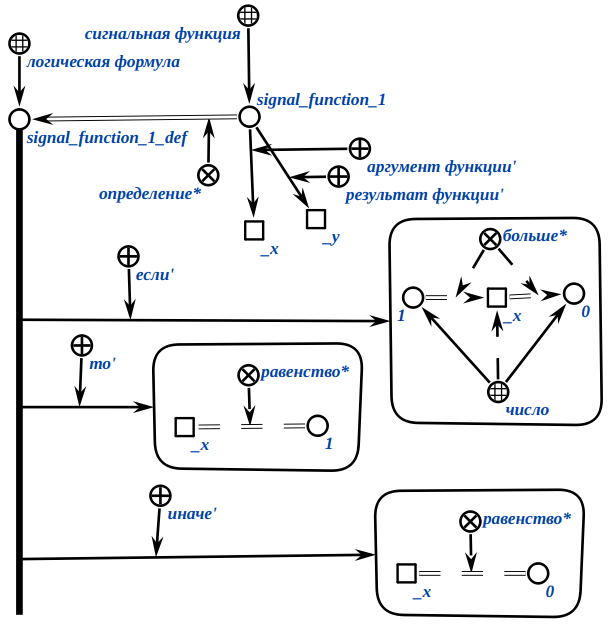
\includegraphics[width=0.5\linewidth]{author/part3/figures/signal_function_def.png}
	\label{fig:signal_function_def}
\end{figure}

Любой агент, интерпретирующий действия с заданными с помощью отношения \textit{функция активации'} аргументами, должен использовать интерпретатор математических функций. использующихся в качестве функций активации.


\section{Логико-семантическая модель ostis-системы автоматизации проектирования искусственных нейронных сетей, семантически совместимых с базами знаний ostis-систем}
\label{sec_chapter_ann_framework}

\begin{SCn}
	\begin{scnrelfromlist}{ключевое понятие}
		\scnitem{действие трансляции условия задачи}
		\scnitem{действие классификации задачи}
		\scnitem{действие поиска подходящей обучающей выборки}
		\scnitem{действие формирования требований к обучающей выборке}
		\scnitem{действие очистки выборки}
		\scnitem{действие выявления содержательных признаков}
		\scnitem{действие трансформации выборки}
		\scnitem{действие разбиения выборки}
		\scnitem{действие выбора класса нейросетевых методов}
		\scnitem{действие формирования спецификации входов и выходов и.н.с.}
		\scnitem{действие выбора метода оптимизации}
		\scnitem{действие выбора минимизируемой функции ошибки}
		\scnitem{действие начальной инициализации и.н.с.}
		\scnitem{действие выбора гиперпараметров и.н.с.}
		\scnitem{метод обучения с учителем}
		\scnitem{метод обучения без учителя}
		\scnitem{действие обучения и.н.с.}
	\end{scnrelfromlist}
\end{SCn}

Наличия \textit{Языка представления нейросетевых методов в базах знаний} и его интерпретатора позволяет обеспечить интерпретацию \textit{нейросетевого метода} в памяти \textit{ostis-системы}. Наличие в единой памяти не только экземпляров методов, но и понятий, их описывающих, создает основу для автоматизации процесса построения нейросетевых методов. В памяти \textit{ostis-системы} хранятся знания о том, методы какого класса могут решить задачу заданного класса, но экземпляров класса этого метода может не быть представлено в системе. На этот случай система должна иметь возможность сообщить пользователю о возможности решения, для которого, однако, необходимо погрузить в систему определенный метод. Так как система хранит в единой памяти задачу и требования к методу ее решения, появляется возможность спроектировать необходимый метод. Для этого необходимо наличие среды проектирования методов соответствующих классов. В случае \textit{нейросетевого метода}, речь идет об интеллектуальной среде построения \textit{нейросетевых методов}.

В основе интеллектуальной среды построения \textit{нейросетевых методов} лежат соответствующие другу другу иерархии действий, задач и методов построения \textit{и.н.с.} Наличие такой иерархии позволит описать язык представления методов построения \textit{и.н.с.} и разработать интерпретатор этого языка.

Построение иерархии соответствующих действий построения \textit{и.н.с.} следует начать с изучения этапов проектирования и обучения \textit{и.н.с.}, которые, в общем случае, выполняют все разработчики и.н.с.:


\textbf{1. Постановка задачи}

Постановка задачи включает в себя описание входных данных (изображения/видео, временные ряды, текст), выходных данных и требований к методу решения (скорость, затраты по памяти и так далее). Также описывается дополнительная информация, которая может помочь в построении метода решения задачи (к примеру, спецификация обучающей выборки, если таковая имеется). Обычно, на данном этапе разработчик и.н.с. определяет класс задачи, формирует требования к обучающей выборке, если она не предоставлена.

Выполнение данного этапа средой проектирования \textit{и.н.с.} подразумевает выполнение следующих действий:
\begin{textitemize}
	\item \textbf{\textit{действие трансляции условия задачи}}. Действие транслирует заданное с помощью \textit{интерфейса ostis-системы} (к примеру, естественно-языкового интерфейса) описание задачи в память ostis-системы. Действие необходимо в случае, когда условие задачи задается пользователем. Необходимо понимать, что описание задачи поступает в базу знаний не только от \textit{пользовательского интерфейса}. К примеру, задача может быть сформулирована самой системой в ходе ее жизнедеятельности.
	Данное действие является общим для всех ostis-систем, поэтому его рассмотрение выходит за рамки рассмотрения процесса построения интеллектуальной среды проектирования \textit{и.н.с.}
	\item \textbf{\textit{действие классификации задачи}}. Действие определяет класс задачи (задача регрессии, детекции, кластеризации и так далее), исходя из описания задачи в базе знаний.
	\item \textbf{\textit{действие поиска подходящей обучающей выборки}}. В базе знаний может храниться набор спецификаций выборок, к которым у ostis-системы есть доступ. Действие производит поиск выборок, которые могут быть использованы в качестве обучающей выборки.
	\item \textbf{\textit{действие формирования требований к обучающей выборке}}. Если обучающая выборка не была предоставлена и не была найдена, то необходимо сформировать описание требований к обучающей выборке, которое можно будет транслировать на язык пользовательского интерфейса и запросить необходимую выборку у пользователя.
\end{textitemize}


\textbf{2. Предобработка выборки: очистка}

На этом этапе обнаруживаются признаки, которые имеют в общем случае некорректные значения (например, для каких-то образов значение признака может иметь неопределенное значение, либо значение, не совпадающее по типу, либо аномально большое или очень маленькое значение, которое встречается в редком числе случаев). Для признаков, имеющих неопределенное значение, может быть применены различные методы устранения, например, такие значения могут быть заменены средним значением этого признака, рассчитанным по всем образам (для непоследовательных данных), либо они могут быть заменены средним значением по соседним образам (в случае временных рядов), либо каким-то фиксированным значением. Радикальная мера решения проблемы --- удаление образов, имеющих неопределенные значения признаков из выборки. Однако его лучше применять, если образов с отсутствующими значениями признаков немного. Для выбросов и аномалий применяются схожие стратегии (но только в том случае, если задача не состоит в прогнозировании этих аномалий).

В интеллектуальной среде проектирования данный этап соответствует выполнению \textbf{\textit{действия очистки выборки}}, которое выполняется в случае обработки выборки, которая ранее не была представлена в памяти системы (к примеру, была получена от пользователя).
Реализация интерпретатора (агента) данного действия требует описания в памяти классификации стратегий очистки данных и реализации методов применения этих стратегий.


\textbf{3. Предобработка выборки: выявление содержательных признаков}

Осуществляется инжиниринг признаков, состоящий в отборе признаков, влияющих на результат работы модели, несодержательные признаки, которые никак не коррелируют с выходом модели, удаляются. Цель этого этапа --- уменьшение размерности пространства признаков для снижения влияния эффекта переобучения на модель.

Для снижения размерности признакового пространства может применяться методы отбора признаков и выделения признаков.

При отборе признаков, осуществляется формирование подмножества из исходных признаков (алгоритм последовательного обратного отбора, рекурсивный алгоритм обратного устранения признаков,  алгоритмы с использованием случайных лесов).

При выделении признаков из набора признаков извлекается информация для построения нового подпространства признаков (алгоритмы с использованием автоэнкодера).

В интеллектуальной среде проектирования данный этап соответствует выполнению \textbf{\textit{действия выявления содержательных признаков}}. Реализация интерпретатора (агента) данного действия требует описания в памяти классификации стратегий уменьшения размерности признакового пространства и реализации методов применения этих стратегий.


\textbf{4. Предобработка выборки: трансформация}

На этом этапе осуществляется подготовка данных к обучению.
Здесь следует уделить особое внимание наличию категориальных признаков, чаще всего заданных строковыми типами. Эти признаки могут быть номинальными и порядковыми. Для кодирования порядковых признаков чаще всего применяют последовательный числовой код (1, 2, 3,...). Для кодирования номинальных такое решение неверно, так как эти признаки равноправны и не могут сравниваться по числовому коду (например, пол --- 0/1). Для номинальных признаков применяется способ прямого кодирования, заключающийся в создании и использовании фиктивных признаков по количеству значений исходного. Например, признак пол (мужской, женский) преобразуется в два новых признака мужской и женский с соответствующими значениями для имеющихся образов.

Масштабирование признаков предполагает приведение значений признаков к одному общему интервалу --- это особенно актуально для признаков, имеющих несоразмерные выборочные средние значения по всем образам --- например, один признак в среднем имеет значение 10.000, а другой 12. Это может проявится в выполнении минимизации только по признаку с наибольшими значениями и плохой сходимости метода обучения. Чаще всего масштабирование соответствует выполнению нормализации на отрезок (min-max нормализация):

\begin{equation*}
	x_{norm}^i = \frac{x^i - x_{min}}{x_{max} - x_{min}}
\end{equation*}
где $x^i$ --- значение признака для отдельно взятого образа \textit{i}, $x_{min}$ --- наименьшее значение для признака, $x_{max}$ --- наибольшее значение для признака.

Другой вариант масштабирования --- применение стандартизации признаков:

\begin{equation*}
	x_{std}^i = \frac{x^i - \mu(x)}{\sigma(x)},
\end{equation*}
$\mu(x)$ --- выборочное среднее отдельного признака, $\sigma(x)$ --- стандартное отклонение.

Стандартизация сохраняет полезную информацию о выбросах в исходных данных и делает алгоритм обучения менее чувствительным к ним.

Дискретизация применяется для перехода от вещественного признака к порядковому за счет кодирования интервалов одним значением (например, если признак отражает возраст человека, то может быть произведена дискретизация значений с выделением определенных возрастных групп, где каждая группа будет кодироваться одним целым числом).

В интеллектуальной среде проектирования данный этап соответствует выполнению \textbf{\textit{действия трансформации выборки}}. Реализация интерпретатора (агента) данного действия требует описания в памяти классификации методов масштабирования признаков и реализации методов применения этих стратегий.


\textbf{5. Разбиение выборки на обучающую, валидационную и тестовую (контрольную)}

Производится разбиение всей выборки данных, на обучающую, тестовую и, в некоторых случаях, валидационную.

Валидационная выборка используется для оценки влияния изменения гиперпараметров на результат обучения и может применяться как дополнительный инструмент для этого наравне с сеточным поиском.

Разбиение проводится в соотношении 3:1:1, в процентах (60/20/20), если валидационная выборка не используется, то 80/20.

В интеллектуальной среде проектирования данный этап соответствует выполнению \textbf{\textit{действия разбиения выборки}}.

Все предыдущие этапы применялись к выборке, последующие этапы относятся к используемым моделям и.н.с.


\textbf{6. Выбор класса нейросетевых методов в соответствии со сформулированной задачей}

На этом этапе осуществляется выбор основной архитектуры и.н.с., которая будет использоваться при обучении. Однако, нужно отметить, что этот выбор относительно условный, то есть исследователь не ограничен использованием только одного типа и.н.с. для решения задачи (как, например, сверточной сети для изображений, поскольку изображения можно обрабатывать и обычным многослойным персептроном). Речь скорее идет именно о рекомендованной архитектуре, но это не исключает использование любых других вариантов архитектур и их сочетаний в рамках одной модели).

Примерами таких рекомендаций являются:
\begin{textitemize}
	\item изображения/видео --- сверхточные нейронные сети;
	\item временные ряды --- многослойные персептроны или рекуррентные сети;
	\item текстовая информация --- многослойные персептроны или рекуррентные сети;
	\item наборы характеристик некоторых объектов (например, спецификации автомобилей) --- многослойный персептрон.
\end{textitemize}

В интеллектуальной среде проектирования данный этап соответствует выполнению \textbf{\textit{действия выбора класса нейросетевых методов}}.


\textbf{7. Формирование спецификации на входные и выходные данные}

Выполняются дополнительные преобразования данных, связанные с изменением структур хранения (например, преобразование многомерного массива в одномерный, конвертация типов)

В интеллектуальной среде проектирования данный этап соответствует выполнению \textbf{\textit{действия формирования спецификации входов и выходов и.н.с.}}.


\textbf{8. Выбор метода оптимизации }

В рамках ПрО и.н.с. описаны следующие методы оптимизации:
\begin{textitemize}
	\item стохастический градиентный спуск (stochastic gradient descent --- SGD);
	\item метод Нестерова;
	\item адаптивный градиент (adaptive gradient --- AdaGrad);
	\item адаптивная оценка момента (adaptive moment estimation --- Adam);
	\item среднеквадратическое распространение (root mean square propagation --- RMSProp).
\end{textitemize}

В интеллектуальной среде проектирования данный этап соответствует выполнению \textbf{\textit{действия выбора метода оптимизации}}.


\textbf{9. Выбор минимизируемой функции ошибки}

На этом этапе задается функция ошибок, которая будет минимизироваться. К примеру, MSE лучше подходит для задач регрессии и для кластеризации, CE --- для классификационных задач.

Данные функции определяются следующим образом:
\begin{equation*}
	MSE = \frac{1}{n} \sum_{i=1}^n (Y_i - \widetilde{Y_i})^2
\end{equation*}
где \textit{n} --- размер обучающей выборки, $Y_i$ --- эталонное значение функции, $\widetilde{Y_i}$ --- результат, полученный НС

\begin{equation*}
	CE = - \frac{1}{n} \sum_{i=1}^n (Y_i\log(\widetilde{Y_i}) + (1-Y_i)\log(1 - \widetilde{Y_i}))
\end{equation*}
(случай 2-классовой классификации)

\begin{equation*}
	CE = - \frac{1}{n} \sum_{i=1}^n \sum_{c=1}^M Y_i^c \log{\widetilde{Y}_i^c}
\end{equation*}
(случай многоклассовой классификации)

В интеллектуальной среде проектирования данный этап соответствует выполнению \textbf{\textit{действия выбора минимизируемой функции ошибки}}.


\textbf{10. Начальная инициализация параметров нейронной сети}

Наиболее часто используемые варианты инициализации весовых коэффициентов и порогов нейронной сети включают:
\begin{textitemize}
	\item Инициализация значениями из равномерного распределения на каком-то небольшом интервале, например, [-0.1, 0.1].
	\item Инициализация значениями из стандартного нормального распределения.
	\item Инициализация по методу Ксавье (см. \scncite{Glorot2010}).

	Применяется для предотвращения резкого уменьшения или увеличения значений выхода нейронных элементов после применения функции активации при прямом прохождении образа через глубокую нейронную сеть. Фактически инициализация этим методом осуществляется посредством выбора значений из равномерного распределения на отрезке $[- \sqrt{6} / \sqrt{n_i+n_{i+1}}, \sqrt{6} / \sqrt{n_i+n_{i+1}}]$, где $n_i$ --- это число входящих связей в данный слой, а $n_i$ --- число исходящих связей из данного слоя. Таким образом, инициализация этим методом проводится для разных слоев нейронной сети из разных отрезков.

	\item Инициализация, полученная из предобученной модели.

	Вариант инициализации, который предполагает использование в качестве \scnqq{стартовой} модели предобученной модели, взятой из некоторого репозитория предобученных моделей, обученную самим исследователем или в процессе работы интеллектуальной системы.

	\item Инициализация по методу Кайминга (см. \scncite{He2015}).

	Данный метод инициализации применяется для решения проблемы \scnqq{затухающего} градиента и \scnqq{взрывающегося}
	градиента. Производится посредством выбора значений из равномерного распределения на отрезке $[-\sqrt{2} / \sqrt{(1+a^2)fan}, \sqrt{2} / \sqrt{(1+a^2)fan}]$,
	где \textit{a} --- угол наклона к оси абсцисс для отрицательной части области определения функции активации типа ReLU (для обычной ReLU функции этот параметр равен 0), $fan$ --- параметр режима работы, который для фазы прямого распространения равен количеству входящих связей (для устранения эффекта \scnqq{взрывающегося} градиента), а для фазы обратного распространения --- количеству выходящих (для устранения эффекта \scnqq{затухающего} градиента).
\end{textitemize}

В интеллектуальной среде проектирования данный этап соответствует выполнению \textbf{\textit{действия начальной инициализации и.н.с.}}.


\textbf{11. Выбора гиперпараметров и.н.с.}

На практике некоторые гиперпараметры (такие как количество слоев, их типы, количество нейронов в слое) часто определяются экспериментально, в процессе итеративного поиска лучшего варианта решения задачи. Хотя способы частично автоматизировать этот процесс существуют, они все же рассчитаны на наличие некоторых предусловий проведения эксперимента, в частности интервалов изменения параметра (например, скорости обучения).

К гиперпараметрам, подбираемым на этом этапе, относятся:
\begin{textitemize}
	\item параметры обучения \textit{и.н.с.} (скорость обучения, моментный параметр, размер мини-батча);
	\item архитектура модели \textit{и.н.с.}, опирающаяся на ранее сформулированные спецификации входных и выходных данных (например, количество нейронов в определенном слое (слоях) или конфигурации целых слоев).
\end{textitemize}

Нахождение оптимальных гиперпараметров может быть получено, например, использованием метода сеточного поиска, который позволяет проверить значения гиперпараметров, взятые с определенным шагом или из определенного интервала (кортежа). С помощью этого метода выбирается оптимальный набор гиперпараметров, который дает лучшие результаты, он используется для последующего дообучения. Или же, если полученные результаты являются приемлемыми, то процесс дальнейшего обучения вообще не проводится. Следует отметить затратность данного метода, так как фактически осуществляется перебор различных значений параметров обучения. Для снижения объема работы применяется метод случайного поиска.

Для оптимизации архитектуры определяются типы слоев нейронной сети, количество нейронных элементов в каждом слое, их характеристики --- функция активации, для сверточных элементов --- размер ядра, а также параметры padding и шаг свертки (stride).
Здесь же может осуществляться оценка не только пользовательского варианта сети, но и предобученной архитектуры. Основное правило при выборе --- количество параметров модели не должно превышать размер обучающей выборки. Для предобученных архитектур это ограничение снимается.

В интеллектуальной среде проектирования данный этап соответствует выполнению \textbf{\textit{действия выбора гипперпараметров и.н.с.}}. Действие использует классификацию и спецификации гиперпараметров \textit{и.н.с.}


\textbf{12. Обучение модели на обучающей выборке}

Производится обучение модели до достижения выбранной точности (оценивается на тестовой выборке) или по другим заданным критериям (достижение заданного количества эпох обучения, неизменность точности на протяжении заданного количества эпох, падение точности на валидационной выборке и так далее).

Приведем классификацию алгоритмов обучения:
\begin{SCn}
	\scnheader{метод обучения и.н.с.}
	\scnsubset{метод}
	\scnsuperset{метод обучения с учителем}
	\begin{scnindent}
		\scntext{explanation}{
			\textbf{\textit{метод обучения с учителем}} --- метод обучения с использованием заданных целевых переменных.
		}
		\scnsuperset{метод обратного распространения ошибки}
		\begin{scnindent}
			\scnidtf{м.о.р.о.}
			\scntext{explanation}{м.о.р.о. использует заданный метод оптимизации и заданную функцию потерь для реализации фазы обратного распространения ошибки и изменения настраиваемых параметров и.н.с. Одним из самых распространенных
			методов оптимизации является метод стохастического градиентного спуска.
			}
			\scntext{explanation}{Следует также отметить, что несмотря на то, что метод отнесен к методам обучения с учителем, в случае
			использования м.о.р.о. для обучения автокодировщиков в классических публикациях он рассматривается как
			метод обучения без учителя, поскольку в данном случае размеченные данные отсутствуют.
			}
		\end{scnindent}
	\end{scnindent}
	\scnsuperset{метод обучения без учителя}
	\begin{scnindent}
		\scntext{explanation}{\textbf{\textit{метод обучения без учителя}} --- метод обучения без использования заданных целевых переменных(в режиме самоорганизации)
		}
		\scntext{explanation}{В ходе выполнения алгоритма метода обучения без учителя выявляются полезные структурные свойства
		набора. Неформально его понимают как метод для извлечения информации из распределения, выборка для которого
		не была вручную аннотирована человеком (см. \scncite{Goodfellow2017}).
		}
	\end{scnindent}
\end{SCn}

В интеллектуальной среде проектирования данный этап соответствует выполнению \textbf{\textit{действия обучения и.н.с.}}. Действие обучения \textit{и.н.с.} --- действие, в ходе которого реализуется определенный метод обучения \textit{и.н.с.} с заданными параметрами обучения \textit{и.н.с.}, методом оптимизации и функцией потерь.

При обучении возможно возникновение следующих проблем:

\begin{textitemize}
	\item \textit{переобучение} --- проблема, возникающая при обучении \textit{и.н.с.}, заключающаяся в том,
	что сеть хорошо адаптируется к паттернам входной активности из обучающей выборки, при этом теряя способность к обобщению.
	Переобучение возникает из-за применения неоправданно сложной модели при обучении \textit{и.н.с.} Это происходит,
	когда количество настраиваемых параметров \textit{и.н.с.} намного больше размера обучающей выборки. Возможные
	варианты решения проблемы заключаются в упрощении модели, увеличении выборки, использовании регуляризации
	(параметр регуляризации, техника dropout и так далее).\\
	Обнаружение переобученности сложнее, чем недообученности. Как правило, для этого применяется
	кросс-валидация на валидационной выборке, позволяющая оценить момент завершения процесса обучения.
	Идеальным вариантом является достижение баланса между переобученностью и недообученностью.

	\item \textit{недообучение} --- проблема, возникающая при обучении  \textit{и.н.с.}, заключающаяся в том,
	что сеть дает одинаково плохие результаты на обучающей и контрольной выборках.
	Чаще всего такого рода проблема возникает при недостаточном времени, затраченном на обучение модели.
	Однако это может быть вызвано и слишком простой архитектурой модели либо малым размером обучающей
	выборки. Соответственно решение, которое может быть принято ML-инженером, заключается в устранении
	этих недостатков: увеличение времени обучения, использование модели с большим числом настраиваемых
	параметров, увеличение размера обучающей выборки, а также уменьшение регуляризации и более тщательный
	отбор признаков для обучающих примеров.
\end{textitemize}

\textit{методом обучения \textit{и.н.с.}} называется процесс итеративного поиска оптимальных значений настраиваемых параметров \textit{и.н.с.}, минимизирующих некоторую заданную функцию потерь.

Стоит отметить, что хотя целью применения метода обучения является минимизация функции потерь, \scnqq{полезность} полученной после обучения модели можно оценить только по достигнутому уровню ее обобщающей способности.

Методы обучения могут быть поделены на две большие группы --- \textit{\textbf{методы обучения с учителем}} и \textit{\textbf{методы обучения без учителя}} (контролируемый и неконтролируемый методы обучения).

\textit{метод обучения с учителем} --- метод обучения с использованием заданных целевых переменных.

Одним из методов обучения с учителем является метод обратного распространения ошибки.

Приведем его описание в виде алгоритма:

\begin{algorithm}[H]
	\KwData{$X$ --- данные, $E_t$ --- желаемый отклик (метки), $E_m$ --- желаемая ошибка (в соответствии с выбранной функцией потерь)}
	\KwResult{обученная нейронная сеть \textit{Net}}
	инициализация весов \textit{W} и порогов \textit{T};\\
	\Repeat{$E<E_m$}{
		\ForEach{$x \in X$, $e \in E_t$}{
			фаза прямого распространения сигнала: вычисляются активации для всех слоев и.н.с.;\\
			фаза обратного распространения ошибки: вычисляются ошибки для последнего слоя и всех предшествующих слоев;\\
			изменение настраиваемых параметров и.н.с. в соответствии с вычисленными ошибками;\\
		}
		вычисление общей ошибки E на данной эпохе;
	}
\end{algorithm}

\textit{метод обратного распространения ошибки} использует заданный метод оптимизации и заданную функцию потерь для реализации фазы обратного распространения ошибки и изменения настраиваемых параметров и.н.с. Одним из самых распространенных методов оптимизации является метод стохастического градиентного спуска. Приведенный метод используется для реализации последовательного варианта обучения.

Следует также отметить, что несмотря на то, что метод отнесен к методам обучения с учителем, в случае
его использования для обучения автокодировщиков в классических публикациях он рассматривается как
метод обучения без учителя, поскольку в данном случае размеченные данные отсутствуют.

\textbf{\textit{метод обучения без учителя}} --- метод обучения без использования заданных целевых переменных (в режиме самоорганизации)

В ходе выполнения алгоритма метода обучения без учителя выявляются полезные структурные свойства
набора. Неформально его понимают как метод для извлечения информации из распределения, выборка для которого
не была вручную аннотирована человеком (см. \scncite{Goodfellow2017}). Метод обучения без учителя может рассматриваться как вспомогательный метод для начальной инициализации настраиваемых параметров и.н.с. В этом случае он является методом предобучения.

Среди методов, применяемых для оптимизации целевой функции можно выделить следующие:

\begin{textitemize}
	\item SGD (стохастический градиентный спуск). В данном методе корректировка настраиваемых параметров и.н.с. выполняется в направлении максимального уменьшения функции стоимости, то есть в направлении, противоположном вектору градиента функции потерь (см. \scncite{Haykin2006}).
	\item Метод Нестерова. Обучение методом стохастического градиентного спуска не редко происходит очень медленно. Импульсный метод позволяет ускорить обучение, особенно в условиях высокой кривизны, небольших, но устойчивых градиентов или зашумленных градиентов. В импульсном методе вычисляется экспоненциально затухающее скользящее среднее прошлых градиентов и продолжается движение в этом направлении. Метод Нестерова является вариантом импульсного алгоритма, в котором градиент вычисляется после применения текущей скорости (см. \scncite{Goodfellow2017}).
	\item AdaGrad: данный метод по отдельности адаптирует скорости обучения всех настраиваемых параметров и.н.с., умножая их на коэффициент, обратно пропорциональный квадратному корню из суммы всех прошлых значений квадрата градиента (см. \scncite{Duchi2011}).
	\item RMSProp. Данный метод является модификацией AdaGrad, которая позволяет улучшить его поведение в невыпуклом случае путем изменения способа агрегирования градиента на экспоненциально взвешенное скользящее среднее. Использование экспоненциально взвешенного скользящего среднего гарантирует повышение скорости сходимости после обнаружения выпуклой впадины, как если бы внутри этой впадины алгоритм AdaGrad был инициализирован заново (см. \scncite{Goodfellow2017});
	\item Adam. Данный метод можно рассматривать как комбинацию RMSProp и AdaGrad (см. \scncite{Kingma2014}). Помимо усредненного первого момента, данный метод использует усредненное значение вторых моментов градиентов.
\end{textitemize}

Отметим, что успешность применения методов оптимизации зависит главным образом от знакомства пользователя с соответствующим алгоритмом (см. \scncite{Goodfellow2017}).

Еще одним важным компонентом, влияющим на процесс обучения, является используемая функция потерь.

\textit{функция потерь} --- функция, используемая для вычисления ошибки, рассчитываемой как разница между фактическим эталонным значением и прогнозируемым значением, получаемым \textit{и.н.с.}

Среди функций потерь, используемые в качестве целевых функций для применяемого метода оптимизации, можно выделить:

\begin{textitemize}
	\item MSE --- средняя квадратичная ошибка\\
	\begin{equation*}
		MSE = \frac{1}{L} \sum_{l=1}^L \sum_{i=1}^m (y_i^l - e_i^l)^2
	\end{equation*}
	где $y_i^l$ --- прогноз модели, $e_i^l$ --- ожидаемый (эталонный) результат, \textit{m} --- размерность выходного вектора, \textit{L} --- объем обучающей выборки;

	\item BCE --- бинарная кросс-энтропия (binary cross-entropy)\\
	\begin{equation*}
		BCE = - \sum_{l=1}^L (e^l \log(y^l) + (1 - e^l)\log(1 - y^l))
	\end{equation*}
	где $y^l$ --- прогноз модели, $e^l$ --- ожидаемый (эталонный) результат: \textit{0} или \textit{1}, \textit{L} --- объем обучающей выборки;
	\item MCE --- мультиклассовая кросс-энтропия (multiclass cross-entropy)\\
	\begin{equation*}
		MCE = - \sum_{l=1}^L \sum_{i=1}^m e_{i}^l \log(y_{i}^l)
	\end{equation*}
	где $y_{i}^l$ --- прогноз модели, $e_i^l$ --- ожидаемый (эталонный результат), \textit{m} --- размерность выходного вектора.
\end{textitemize}

Отметим, что для бинарной кросс-энтропии в выходном слое \textit{и.н.с.} будет находиться один нейрон, а для для мультиклассовой кросс-энтропии количество нейронов в выходном \textit{слое и.н.с.} совпадает с количеством классов.

Для решения задачи классификации рекомендуется использовать бинарную или мультиклассовую кросс-энтропийную функцию потерь, для решения задачи регрессии рекомендуется использовать среднюю квадратичную ошибку.

Действие обучения \textit{и.н.с.} можно проиллюстрировать следующим изображением \textit{\nameref{fig:ann_training_nn_scg}}.

\begin{figure}[H]
	\caption{SCg-текст. Действие обучения и.н.с.}
	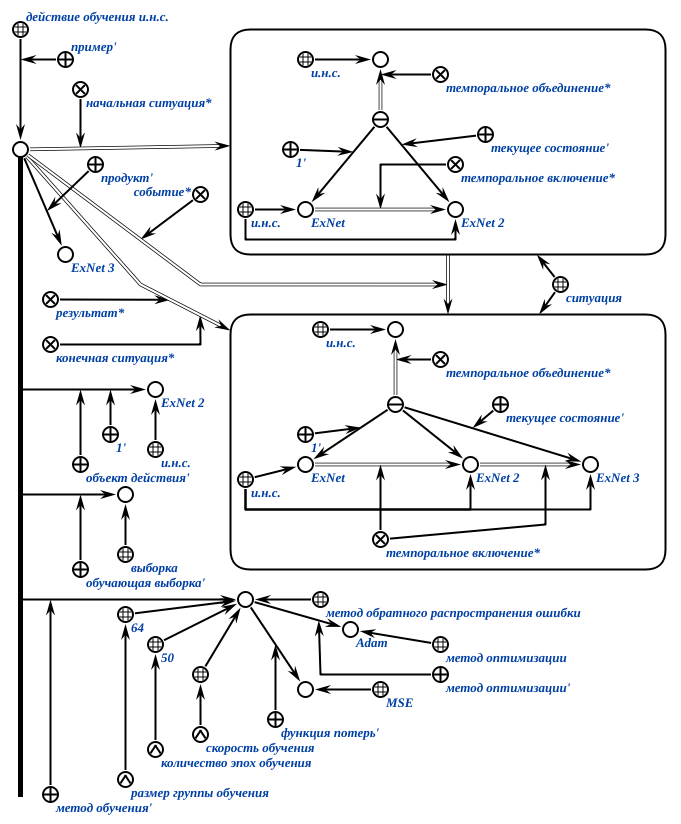
\includegraphics[scale=0.7]{author/part3/figures/ann_training_nn_scg.png}
	\label{fig:ann_training_nn_scg}
\end{figure}

\textbf{13. Оценка эффективности и.н.с}

После выполнения обучения осуществляется оценка полученной модели с помощью метрик оценки качества.

Далее результат оценки может быть визуализирован с помощью матрицы ошибок (confusion matrix) и ROC-кривой.

Матрица ошибок представляется собой матрицу (см. \nameref{fig:conf_matrix}), в которую помещены сведения о числе истинно-положительных, истинно-отрицательных, ложно-положительных и ложно-отрицательных предсказаниях классификатора.

\begin{figure}[H]
	\caption{Рисунок. Матрица ошибок}
	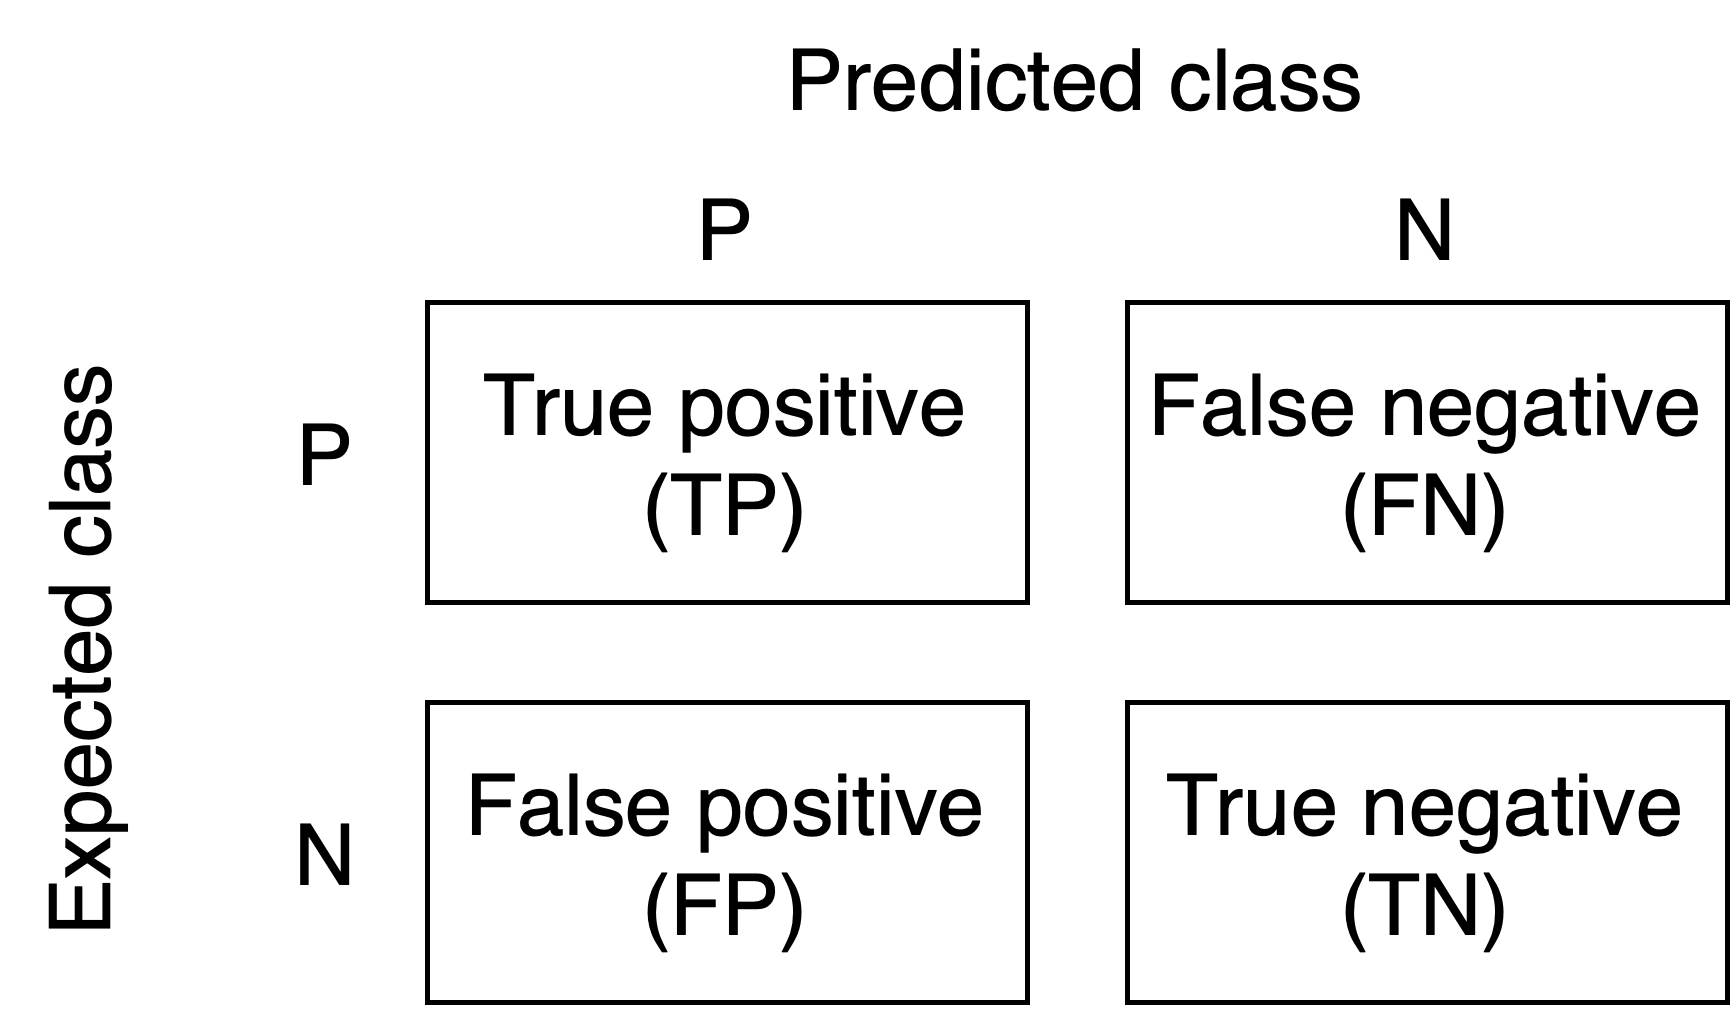
\includegraphics[width=0.4\textwidth]{author/part3/figures/conf_matrix.png}
	\label{fig:conf_matrix}
\end{figure}

\textit{ROC-кривая} (receiver operating characteristic) --- это график, в котором, основываясь на заданном пороге решения классификатора, рассчитываются доли ложноположительных и истинно положительных исходов. Основываясь на ROC-кривой, высчитывается AUC-показатель (площадь под кривой), которая используется в качестве характеристики качества модели.

В интеллектуальной среде проектирования данный этап соответствует выполнению \textit{действия оценки эффективности и.н.с.}.

Рассмотрим пример выполнения описанных этапов разработчиком для конкретной задачи --- \textit{классификации цифр из выборки рукописных цифр MNIST}:

\begin{textitemize}
\item Исходными данными задачи является: выборка из 70.000 изображений, предварительно разделенная на обучающую (60.000 изображений) и контрольную (10.000 изображений) выборки. Каждое изображение представлено двумерным массивом 28Х28 чисел из интервала [0, 255], числа представляют определенный оттенок серого цвета. Помимо этого каждому изображению соответствует метка класса, соответствующая конкретной цифре от 0 до 9.

Ставится задача: \textit{обучить модель, которая будет принимать на вход двумерный массив данных и возвращать метку класса, соответствующей распознанной цифре.}

Таким образом, тип решаемой задачи --- \textbf{классификационная}, природа данных задачи --- \textbf{изображения}.

\item В рассматриваемой выборке отсутствуют аномалии, ошибочные данные, признаки с отсутствующими значениями.

\item В рассматриваемой задаче отсутствуют несодержательные признаки.

\item В качестве метода предобработки данных используем масштабирование признаков, а именно нормализацию на отрезок [0, 1].

\item Выполним разбиение обучающей части данных на обучающую и валидационную выборки в соотношении 4:1 (48.000 в обучающей и 12.000 в валидационной).

\item Так как выборка включает в себя изображения, будем использовать сверточную нейронную сеть.

\item Не требуется.

\item В качестве оптимизационного алгоритма будем использовать метод стохастического градиентного спуска (SGD).

\item Так как решается задача классификации, выберем в качестве минимизируемой функции кросс-энтропийную функцию потерь.

\item В качестве начальной инициализации будем использовать инициализацию по методу Кайминга.

\item На предыдущих этапах было определено, что для решения задачи будет использоваться сверточная нейронная сеть. При использовании one-hot кодирования в последнем полносвязном слое будет 10 нейронов по числу классов в задаче.

Для упрощения будем использовать архитектуру, изображенную на \textit{\nameref{fig:model}}, не содержащую промежуточные слои.

\begin{figure}[H]
	\caption{Рисунок. Архитектура и.н.с., решающая задачу классификации цифр}
	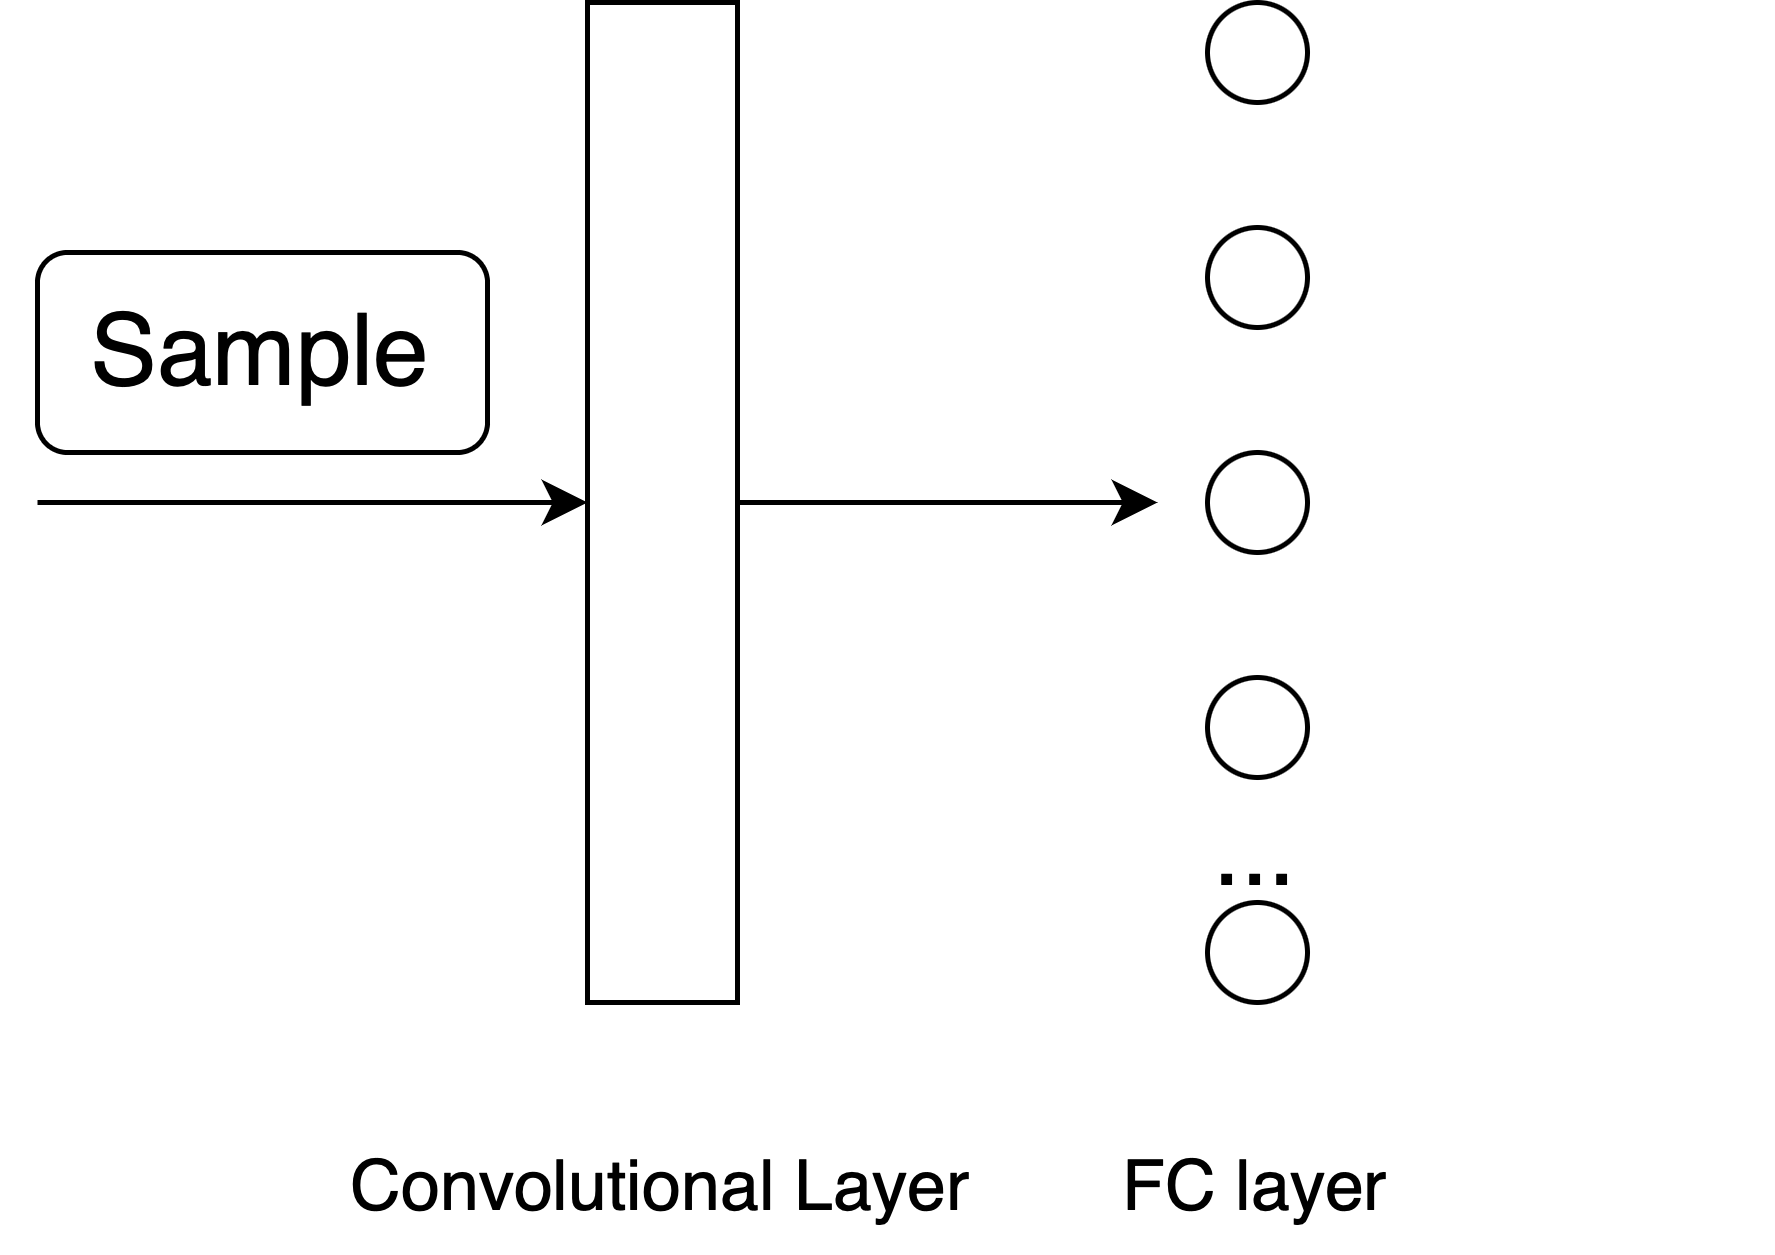
\includegraphics[width=0.4\textwidth]{author/part3/figures/model.png}
	\label{fig:model}
\end{figure}

Для нахождения оптимального набора гиперпараметров будем применять метод случайного поиска.

Перечислим кортежи, из которых будут сэмплироваться гиперпараметры:
\begin{textitemize}
	\item Скорость обучения --- (0.9, 0.1, 0.01, 0.001);
	\item Количество нейронов в сверточном слое --- (5, 10, 15, 20);
	\item Размер ядра свертки --- (3, 5, 7, 9);
	\item Моментный параметр --- (0, 0.5, 0.9);
	\item Размер мини-батча --- (16, 32, 64, 128).
\end{textitemize}

После определения данных параметров и оценки эффективности работы алгоритма, получим следующую таблицу:

\begin{table}[ht]
	\caption{Таблица. Результаты решения задачи \\(используемые сокращения: mbs --- mini-batch size, ks --- kernel size, lr --- learning rate, cnc --- convolutional neurons count, acc --- accuracy, it --- iterations count)}
	\centering
	\begin{tabular}{c c c c c c c c}
		\hline\hline
		\# & mbs & ks & lr    & momentum & cnc & acc    & it \\ [0.5ex] % inserts table %heading
		\hline
		1        & 128 & 3  & 0.001 & 0.5      & 10  & 0.9033 & 10 \\
		2        & 64  & 9  & 0.9   & 0        & 15  & 0.1039 & 1  \\
		3        & 32  & 3  & 0.01  & 0.5      & 20  & 0.9741 & 10 \\
		4        & 32  & 7  & 0.01  & 0.5      & 15  & 0.9794 & 10 \\
		5        & 16  & 9  & 0.001 & 0.5      & 20  & 0.9189 & 2  \\
		6        & 64  & 3  & 0.1   & 0.5      & 10  & 0.9736 & 10 \\
		7        & 64  & 7  & 0.001 & 0.9      & 15  & 0.9007 & 1  \\
		8        & 32  & 9  & 0.1   & 0.5      & 5   & 0.9806 & 10 \\
		9        & 128 & 5  & 0.1   & 0.5      & 20  & 0.98   & 10 \\
		10       & 32  & 9  & 0.01  & 0.9      & 5   & 0.9806 & 10 \\
		11       & 128 & 3  & 0.001 & 0.9      & 10  & 0.893  & 1  \\
		12       & 32  & 5  & 0.9   & 0.9      & 20  & 0.1008 & 1  \\
		13       & 16  & 9  & 0.9   & 0.5      & 20  & 0.0976 & 1  \\
		14       & 32  & 7  & 0.9   & 0.9      & 15  & 0.0932 & 1  \\
		15       & 128 & 5  & 0.01  & 0.5      & 20  & 0.9197 & 2  \\
		16       & 16  & 3  & 0.001 & 0.5      & 10  & 0.904  & 1  \\
		17       & 16  & 9  & 0.001 & 0        & 20  & 0.8866 & 1  \\
		18       & 128 & 9  & 0.1   & 0.5      & 5   & 0.9793 & 10 \\
		19       & 128 & 3  & 0.001 & 0        & 10  & 0.6697 & 1  \\
		20       & 16  & 3  & 0.1   & 0        & 15  & 0.9729 & 4  \\
		21       & 32  & 7  & 0.9   & 0.5      & 15  & 0.1048 & 1  \\
		22       & 128 & 7  & 0.9   & 0        & 15  & 0.1113 & 1  \\
		23       & 64  & 9  & 0.01  & 0.5      & 10  & 0.9482 & 2  \\
		24       & 16  & 7  & 0.9   & 0        & 20  & 0.0985 & 1  \\
		25       & 16  & 3  & 0.1   & 0.5      & 5   & 0.9558 & 2  \\
		26       & 64  & 7  & 0.01  & 0.9      & 15  & 0.9839 & 10 \\
		27       & 16  & 7  & 0.1   & 0        & 10  & 0.9836 & 10 \\
		28       & 16  & 5  & 0.01  & 0        & 20  & 0.9608 & 2  \\
		29       & 16  & 5  & 0.01  & 0.9      & 20  & 0.9847 & 10 \\
		30       & 32  & 5  & 0.01  & 0.5      & 15  & 0.9532 & 2  \\
		\hline
	\end{tabular}
	\label{table:nonlin}
\end{table}

Можно заметить, что лучший результат (acc = 0.9839) по обобщающей способности на валидационной выборке был получен при следующих параметрах: mbs = 64, ks = 7, lr = 0.01, momentum = 0.9, cnc = 15.

\item В качестве критерия останова нами был выбран самый простой критерий по достижению заданного количества эпох обучения. Дообучение не проводилось, для оценки обобщающей способности использовалась модель, полученная после выполнения процедуры подбора гиперпараметров. Обобщающая способность на тестовой выборке составила \textbf{0.9853}, то есть \textbf{98.53\%}.

\item Построив матрицу ошибок на основании обученной модели и тестовой выборки, получим результат, проиллюстрированный на рис. \nameref{fig:conf_matrix_result}

\begin{figure}[H]
	\caption{Рисунок. Матрица ошибок для задачи MNIST}
	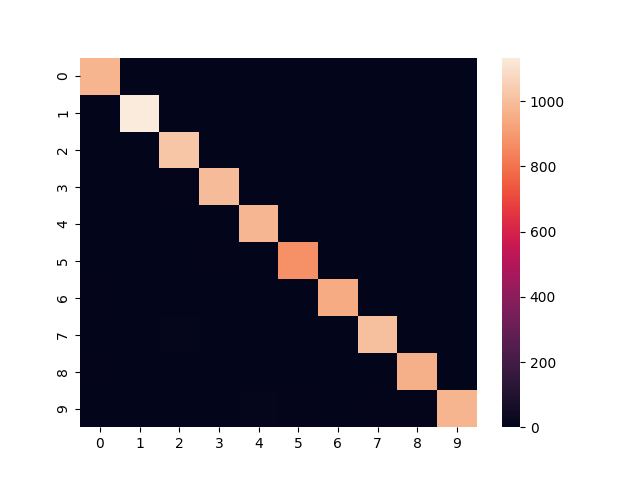
\includegraphics[width=0.55\textwidth]{author/part3/figures/conf_matrix_result.png}
	\label{fig:conf_matrix_result}
\end{figure}

Мы получили матрицу с явно выраженным диагональным преобладанием, таким образом полученная модель делает относительно небольшое число ошибок.
\end{textitemize}

Исходя из анализа этапов построения и.н.с., которые выполняют разработчики, можно вывести следующую классификацию действий по построению и.н.с.:

\begin{SCn}
	\scnheader{действие по построению и.н.с.}
	\begin{scnrelfromset}{декомпозиция}
		\scnitem{действие по обработке выборки}
		\begin{scnrelfromset}{декомпозиция}
			\scnitem{действие поиска подходящей обучающей выборки}
			\scnitem{действие формирования требований к обучающей выборке}
			\scnitem{действие очистки выборки}
			\scnitem{действие выявления содержательных признаков}
			\scnitem{действие трансформации выборки}
			\scnitem{действие разбиения выборки}
		\end{scnrelfromset}

		\scnitem{действие по проектированию и.н.с.}
		\begin{scnrelfromset}{декомпозиция}
			\scnitem{действие выбора класса нейросетевых методов}
			\scnitem{действие формирования спецификации входов и выходов и.н.с.}
		\end{scnrelfromset}

		\scnitem{действие обучения и.н.с.}
		\begin{scnrelfromset}{декомпозиция}
			\scnitem{действие выбора метода оптимизации}
			\scnitem{действие выбора минимизируемой функции ошибки}
			\scnitem{действие начальной инициализации и.н.с.}
			\scnitem{действие выбора гиперпараметров и.н.с.}
			\scnitem{действие обучения и.н.с.}
			\scnitem{действие оценки эффективности и.н.с.}
		\end{scnrelfromset}
	\end{scnrelfromset}
\end{SCn}

Реализация интерпретатора описанных в данной главе действий по построению \textit{и.н.с.} и описания в базе знаний экспертных знаний разработчиков\textit{ и.н.с.} (а значит реализация интеллектуальной среды проектирования \textit{и.н.с.}) позволит автоматически, исходя из описания задачи, генерировать нейросетевые методы в памяти \textit{ostis-системы}, что является одним из ключевых направлений дальнейшего развития конвергенции и интеграции и.н.с. с базами знаний.

Так как в результате действий по построению \textit{и.н.с.} объект этих действий, конкретная \textit{и.н.с.}, может существенно меняться (меняется конфигурация сети, ее весовые коэффициенты), то \textit{и.н.с.} представляется в базе знаний как темпоральное объединение всех ее версий. Каждая версия является \textit{и.н.с.} и темпоральной сущностью. На множестве этих темпоральных сущностей задается темпоральная последовательность с указанием первой и последней версии. Для каждой версии описываются специфичные знания.

Общие для всех версий знания описываются для \textit{и.н.с.}, являющейся темпоральным объединением всех версий (рисунок \nameref{fig:temporal_neural_network_scg})

\begin{figure}[H]
	\caption{SCg-текст. Темпоральность нейронной сети}
	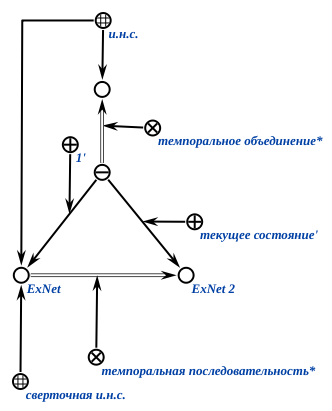
\includegraphics[scale=0.8]{author/part3/figures/temporal_neural_network_scg.png}
	\label{fig:temporal_neural_network_scg}
\end{figure}

Далее более подробно рассмотрим действие по обучению \textit{и.н.с.} и сделаем обзор основных методов, применяемых для обучения.

\section*{Заключение к Главе \ref{chapter_ann}}
В главе описан подход к \textit{интеграции и конвергенции искусственных нейронных сетей с базами знаний} в \textit{интеллектуальных компьютерных системах нового поколения} с помощью представления и интерпретации \textit{искусственной нейронной сети} в \textit{базе знаний}.

Описаны \textit{Синтаксис, Денотационная и Операционная семантика Языка представления нейросетевых методов в базах знаний}, который позволяет представить и интерпретировать в памяти интеллектуальной системы любую \textit{и.н.с.} Наличие такого языка порождает семантическую совместимость нейросетевого метода с другими методами, представленными в памяти системы, что позволяет анализировать саму \textit{и.н.с.} и этапы ее работы любыми другими методами системы.

Так же наличие языка представления нейросетевых методов позволяет описывать в памяти системы экспертные знания разработчиков \textit{и.н.с.} В главе приведены этапы построения \textit{и.н.с.}, которые выполняют разработчики \textit{и.н.с.} На основании этих этапов, c целью проектирования интеллектуальной среды построения \textit{нейросетевых методов}, в \textit{базе знаний} были классифицированы и описаны действия по построению \textit{и.н.с.}

Проектирования и реализация интеллектуальной среды построения \textit{и.н.с.} в \textit{базе знаний} системы является одним из двух основных направлений дальнейшего развития работу по конвергенции и интеграции и.н.с. с базами знаний.

Вторым основным направлением является разработка подхода к обработке фрагментов \textit{базы знаний} с помощью \textit{и.н.с.}, для чего необходимо разработать универсальный алгоритм взаимно-однозначного соответствия фрагментов базы знаний и входных векторов \textit{и.н.с.} Язык представления знаний способен представить любое знание. Наличие в системе нейросетевого метода, способного принимать на вход фрагменты знаний, позволит решить новые, слабо изученные классы задач. 
